\documentclass[twoside]{book}

% Packages required by doxygen
\usepackage{fixltx2e}
\usepackage{calc}
\usepackage{doxygen}
\usepackage[export]{adjustbox} % also loads graphicx
\usepackage{graphicx}
\usepackage[utf8]{inputenc}
\usepackage{makeidx}
\usepackage{multicol}
\usepackage{multirow}
\PassOptionsToPackage{warn}{textcomp}
\usepackage{textcomp}
\usepackage[nointegrals]{wasysym}
\usepackage[table]{xcolor}

% Font selection
\usepackage[T1]{fontenc}
\usepackage[scaled=.90]{helvet}
\usepackage{courier}
\usepackage{amssymb}
\usepackage{sectsty}
\renewcommand{\familydefault}{\sfdefault}
\allsectionsfont{%
  \fontseries{bc}\selectfont%
  \color{darkgray}%
}
\renewcommand{\DoxyLabelFont}{%
  \fontseries{bc}\selectfont%
  \color{darkgray}%
}
\newcommand{\+}{\discretionary{\mbox{\scriptsize$\hookleftarrow$}}{}{}}

% Page & text layout
\usepackage{geometry}
\geometry{%
  a4paper,%
  top=2.5cm,%
  bottom=2.5cm,%
  left=2.5cm,%
  right=2.5cm%
}
\tolerance=750
\hfuzz=15pt
\hbadness=750
\setlength{\emergencystretch}{15pt}
\setlength{\parindent}{0cm}
\setlength{\parskip}{3ex plus 2ex minus 2ex}
\makeatletter
\renewcommand{\paragraph}{%
  \@startsection{paragraph}{4}{0ex}{-1.0ex}{1.0ex}{%
    \normalfont\normalsize\bfseries\SS@parafont%
  }%
}
\renewcommand{\subparagraph}{%
  \@startsection{subparagraph}{5}{0ex}{-1.0ex}{1.0ex}{%
    \normalfont\normalsize\bfseries\SS@subparafont%
  }%
}
\makeatother

% Headers & footers
\usepackage{fancyhdr}
\pagestyle{fancyplain}
\fancyhead[LE]{\fancyplain{}{\bfseries\thepage}}
\fancyhead[CE]{\fancyplain{}{}}
\fancyhead[RE]{\fancyplain{}{\bfseries\leftmark}}
\fancyhead[LO]{\fancyplain{}{\bfseries\rightmark}}
\fancyhead[CO]{\fancyplain{}{}}
\fancyhead[RO]{\fancyplain{}{\bfseries\thepage}}
\fancyfoot[LE]{\fancyplain{}{}}
\fancyfoot[CE]{\fancyplain{}{}}
\fancyfoot[RE]{\fancyplain{}{\bfseries\scriptsize Generated by Doxygen }}
\fancyfoot[LO]{\fancyplain{}{\bfseries\scriptsize Generated by Doxygen }}
\fancyfoot[CO]{\fancyplain{}{}}
\fancyfoot[RO]{\fancyplain{}{}}
\renewcommand{\footrulewidth}{0.4pt}
\renewcommand{\chaptermark}[1]{%
  \markboth{#1}{}%
}
\renewcommand{\sectionmark}[1]{%
  \markright{\thesection\ #1}%
}

% Indices & bibliography
\usepackage{natbib}
\usepackage[titles]{tocloft}
\setcounter{tocdepth}{3}
\setcounter{secnumdepth}{5}
\makeindex

% Hyperlinks (required, but should be loaded last)
\usepackage{ifpdf}
\ifpdf
  \usepackage[pdftex,pagebackref=true]{hyperref}
\else
  \usepackage[ps2pdf,pagebackref=true]{hyperref}
\fi
\hypersetup{%
  colorlinks=true,%
  linkcolor=blue,%
  citecolor=blue,%
  unicode%
}

% Custom commands
\newcommand{\clearemptydoublepage}{%
  \newpage{\pagestyle{empty}\cleardoublepage}%
}

\usepackage{caption}
\captionsetup{labelsep=space,justification=centering,font={bf},singlelinecheck=off,skip=4pt,position=top}

%===== C O N T E N T S =====

\begin{document}

% Titlepage & ToC
\hypersetup{pageanchor=false,
             bookmarksnumbered=true,
             pdfencoding=unicode
            }
\pagenumbering{alph}
\begin{titlepage}
\vspace*{7cm}
\begin{center}%
{\Large libarsc }\\
\vspace*{1cm}
{\large Generated by Doxygen 1.8.14}\\
\end{center}
\end{titlepage}
\clearemptydoublepage
\pagenumbering{roman}
\tableofcontents
\clearemptydoublepage
\pagenumbering{arabic}
\hypersetup{pageanchor=true}

%--- Begin generated contents ---
\chapter{Hierarchical Index}
\section{Class Hierarchy}
This inheritance list is sorted roughly, but not completely, alphabetically\+:\begin{DoxyCompactList}
\item Exception\begin{DoxyCompactList}
\item \contentsline{section}{arsc.\+exceptions.\+Chunk\+Header\+Wrong\+Type\+Exception}{\pageref{classarsc_1_1exceptions_1_1ChunkHeaderWrongTypeException}}{}
\item \contentsline{section}{arsc.\+exceptions.\+Wrong\+Type\+Exception}{\pageref{classarsc_1_1exceptions_1_1WrongTypeException}}{}
\end{DoxyCompactList}
\item \contentsline{section}{arsc.\+config.\+Res\+Table\+\_\+config.\+Imsi}{\pageref{classarsc_1_1config_1_1ResTable__config_1_1Imsi}}{}
\item \contentsline{section}{arsc.\+config.\+Res\+Table\+\_\+config.\+Input}{\pageref{classarsc_1_1config_1_1ResTable__config_1_1Input}}{}
\item \contentsline{section}{arsc.\+config.\+Res\+Table\+\_\+config.\+Locale}{\pageref{classarsc_1_1config_1_1ResTable__config_1_1Locale}}{}
\item \contentsline{section}{arsc.\+chunk.\+Res\+Chunk\+\_\+header}{\pageref{classarsc_1_1chunk_1_1ResChunk__header}}{}
\item \contentsline{section}{arsc.\+stringpool.\+Res\+String\+Pool}{\pageref{classarsc_1_1stringpool_1_1ResStringPool}}{}
\item \contentsline{section}{arsc.\+stringpool.\+Res\+String\+Pool\+\_\+header}{\pageref{classarsc_1_1stringpool_1_1ResStringPool__header}}{}
\item \contentsline{section}{arsc.\+arsc.\+Res\+Table}{\pageref{classarsc_1_1arsc_1_1ResTable}}{}
\item \contentsline{section}{arsc.\+config.\+Res\+Table\+\_\+config}{\pageref{classarsc_1_1config_1_1ResTable__config}}{}
\item \contentsline{section}{arsc.\+table.\+Res\+Table\+\_\+header}{\pageref{classarsc_1_1table_1_1ResTable__header}}{}
\item \contentsline{section}{arsc.\+package.\+Res\+Table\+\_\+package}{\pageref{classarsc_1_1package_1_1ResTable__package}}{}
\item \contentsline{section}{arsc.\+package.\+Res\+Table\+\_\+package\+\_\+header}{\pageref{classarsc_1_1package_1_1ResTable__package__header}}{}
\item \contentsline{section}{arsc.\+tabletype.\+Res\+Table\+\_\+type}{\pageref{classarsc_1_1tabletype_1_1ResTable__type}}{}
\item \contentsline{section}{arsc.\+tabletype.\+Res\+Table\+\_\+type\+\_\+header}{\pageref{classarsc_1_1tabletype_1_1ResTable__type__header}}{}
\item \contentsline{section}{arsc.\+tabletype.\+Res\+Table\+\_\+type\+Spec}{\pageref{classarsc_1_1tabletype_1_1ResTable__typeSpec}}{}
\item \contentsline{section}{arsc.\+tabletype.\+Res\+Table\+\_\+type\+Spec\+\_\+header}{\pageref{classarsc_1_1tabletype_1_1ResTable__typeSpec__header}}{}
\item \contentsline{section}{arsc.\+config.\+Res\+Table\+\_\+config.\+Screen\+Config}{\pageref{classarsc_1_1config_1_1ResTable__config_1_1ScreenConfig}}{}
\item \contentsline{section}{arsc.\+config.\+Res\+Table\+\_\+config.\+Screen\+Size}{\pageref{classarsc_1_1config_1_1ResTable__config_1_1ScreenSize}}{}
\item \contentsline{section}{arsc.\+config.\+Res\+Table\+\_\+config.\+Screen\+Size\+Dp}{\pageref{classarsc_1_1config_1_1ResTable__config_1_1ScreenSizeDp}}{}
\item \contentsline{section}{arsc.\+config.\+Res\+Table\+\_\+config.\+Screen\+Type}{\pageref{classarsc_1_1config_1_1ResTable__config_1_1ScreenType}}{}
\item \contentsline{section}{arsc.\+type.\+uint16.\+uint16}{\pageref{classarsc_1_1type_1_1uint16_1_1uint16}}{}
\item \contentsline{section}{arsc.\+type.\+uint24.\+uint24}{\pageref{classarsc_1_1type_1_1uint24_1_1uint24}}{}
\item \contentsline{section}{arsc.\+type.\+uint32.\+uint32}{\pageref{classarsc_1_1type_1_1uint32_1_1uint32}}{}
\item \contentsline{section}{arsc.\+type.\+uint64.\+uint64}{\pageref{classarsc_1_1type_1_1uint64_1_1uint64}}{}
\item \contentsline{section}{arsc.\+type.\+uint8.\+uint8}{\pageref{classarsc_1_1type_1_1uint8_1_1uint8}}{}
\item \contentsline{section}{arsc.\+config.\+Res\+Table\+\_\+config.\+Version}{\pageref{classarsc_1_1config_1_1ResTable__config_1_1Version}}{}
\item Int\+Enum\begin{DoxyCompactList}
\item \contentsline{section}{arsc.\+type.\+enum.\+Enum}{\pageref{classarsc_1_1type_1_1enum_1_1Enum}}{}
\begin{DoxyCompactList}
\item \contentsline{section}{arsc.\+external.\+configuration.\+A\+Configuration}{\pageref{classarsc_1_1external_1_1configuration_1_1AConfiguration}}{}
\item \contentsline{section}{arsc.\+types.\+Resource\+Type}{\pageref{classarsc_1_1types_1_1ResourceType}}{}
\end{DoxyCompactList}
\end{DoxyCompactList}
\item Int\+Flag\begin{DoxyCompactList}
\item \contentsline{section}{arsc.\+type.\+flag.\+Flag}{\pageref{classarsc_1_1type_1_1flag_1_1Flag}}{}
\begin{DoxyCompactList}
\item \contentsline{section}{arsc.\+config.\+Res\+Table\+\_\+config.\+Config}{\pageref{classarsc_1_1config_1_1ResTable__config_1_1Config}}{}
\item \contentsline{section}{arsc.\+stringpool.\+Res\+String\+Pool\+\_\+header.\+Flags}{\pageref{classarsc_1_1stringpool_1_1ResStringPool__header_1_1Flags}}{}
\end{DoxyCompactList}
\end{DoxyCompactList}
\end{DoxyCompactList}

\chapter{Class Index}
\section{Class List}
Here are the classes, structs, unions and interfaces with brief descriptions\+:\begin{DoxyCompactList}
\item\contentsline{section}{\mbox{\hyperlink{classarsc_1_1external_1_1configuration_1_1AConfiguration}{arsc.\+external.\+configuration.\+A\+Configuration}} }{\pageref{classarsc_1_1external_1_1configuration_1_1AConfiguration}}{}
\item\contentsline{section}{\mbox{\hyperlink{classarsc_1_1exceptions_1_1ChunkHeaderWrongTypeException}{arsc.\+exceptions.\+Chunk\+Header\+Wrong\+Type\+Exception}} }{\pageref{classarsc_1_1exceptions_1_1ChunkHeaderWrongTypeException}}{}
\item\contentsline{section}{\mbox{\hyperlink{classarsc_1_1config_1_1ResTable__config_1_1Config}{arsc.\+config.\+Res\+Table\+\_\+config.\+Config}} }{\pageref{classarsc_1_1config_1_1ResTable__config_1_1Config}}{}
\item\contentsline{section}{\mbox{\hyperlink{classarsc_1_1type_1_1enum_1_1Enum}{arsc.\+type.\+enum.\+Enum}} }{\pageref{classarsc_1_1type_1_1enum_1_1Enum}}{}
\item\contentsline{section}{\mbox{\hyperlink{classarsc_1_1type_1_1flag_1_1Flag}{arsc.\+type.\+flag.\+Flag}} }{\pageref{classarsc_1_1type_1_1flag_1_1Flag}}{}
\item\contentsline{section}{\mbox{\hyperlink{classarsc_1_1stringpool_1_1ResStringPool__header_1_1Flags}{arsc.\+stringpool.\+Res\+String\+Pool\+\_\+header.\+Flags}} }{\pageref{classarsc_1_1stringpool_1_1ResStringPool__header_1_1Flags}}{}
\item\contentsline{section}{\mbox{\hyperlink{classarsc_1_1config_1_1ResTable__config_1_1Imsi}{arsc.\+config.\+Res\+Table\+\_\+config.\+Imsi}} \\*Filter based on M\+CC and M\+NC }{\pageref{classarsc_1_1config_1_1ResTable__config_1_1Imsi}}{}
\item\contentsline{section}{\mbox{\hyperlink{classarsc_1_1config_1_1ResTable__config_1_1Input}{arsc.\+config.\+Res\+Table\+\_\+config.\+Input}} }{\pageref{classarsc_1_1config_1_1ResTable__config_1_1Input}}{}
\item\contentsline{section}{\mbox{\hyperlink{classarsc_1_1config_1_1ResTable__config_1_1Locale}{arsc.\+config.\+Res\+Table\+\_\+config.\+Locale}} \\*Filter based on language and country }{\pageref{classarsc_1_1config_1_1ResTable__config_1_1Locale}}{}
\item\contentsline{section}{\mbox{\hyperlink{classarsc_1_1chunk_1_1ResChunk__header}{arsc.\+chunk.\+Res\+Chunk\+\_\+header}} \\*Header that appears at the front of every data chunk in a resource }{\pageref{classarsc_1_1chunk_1_1ResChunk__header}}{}
\item\contentsline{section}{\mbox{\hyperlink{classarsc_1_1types_1_1ResourceType}{arsc.\+types.\+Resource\+Type}} }{\pageref{classarsc_1_1types_1_1ResourceType}}{}
\item\contentsline{section}{\mbox{\hyperlink{classarsc_1_1stringpool_1_1ResStringPool}{arsc.\+stringpool.\+Res\+String\+Pool}} }{\pageref{classarsc_1_1stringpool_1_1ResStringPool}}{}
\item\contentsline{section}{\mbox{\hyperlink{classarsc_1_1stringpool_1_1ResStringPool__header}{arsc.\+stringpool.\+Res\+String\+Pool\+\_\+header}} \\*Definition for a pool of strings }{\pageref{classarsc_1_1stringpool_1_1ResStringPool__header}}{}
\item\contentsline{section}{\mbox{\hyperlink{classarsc_1_1arsc_1_1ResTable}{arsc.\+arsc.\+Res\+Table}} }{\pageref{classarsc_1_1arsc_1_1ResTable}}{}
\item\contentsline{section}{\mbox{\hyperlink{classarsc_1_1config_1_1ResTable__config}{arsc.\+config.\+Res\+Table\+\_\+config}} \\*Describes current Res\+Table\+\_\+type configuration }{\pageref{classarsc_1_1config_1_1ResTable__config}}{}
\item\contentsline{section}{\mbox{\hyperlink{classarsc_1_1table_1_1ResTable__header}{arsc.\+table.\+Res\+Table\+\_\+header}} \\*Header for a resource table }{\pageref{classarsc_1_1table_1_1ResTable__header}}{}
\item\contentsline{section}{\mbox{\hyperlink{classarsc_1_1package_1_1ResTable__package}{arsc.\+package.\+Res\+Table\+\_\+package}} \\*Describes whole package, together with its content }{\pageref{classarsc_1_1package_1_1ResTable__package}}{}
\item\contentsline{section}{\mbox{\hyperlink{classarsc_1_1package_1_1ResTable__package__header}{arsc.\+package.\+Res\+Table\+\_\+package\+\_\+header}} \\*A collection of resource data types within a package }{\pageref{classarsc_1_1package_1_1ResTable__package__header}}{}
\item\contentsline{section}{\mbox{\hyperlink{classarsc_1_1tabletype_1_1ResTable__type}{arsc.\+tabletype.\+Res\+Table\+\_\+type}} }{\pageref{classarsc_1_1tabletype_1_1ResTable__type}}{}
\item\contentsline{section}{\mbox{\hyperlink{classarsc_1_1tabletype_1_1ResTable__type__header}{arsc.\+tabletype.\+Res\+Table\+\_\+type\+\_\+header}} \\*A collection of resource entries for a particular resource data type }{\pageref{classarsc_1_1tabletype_1_1ResTable__type__header}}{}
\item\contentsline{section}{\mbox{\hyperlink{classarsc_1_1tabletype_1_1ResTable__typeSpec}{arsc.\+tabletype.\+Res\+Table\+\_\+type\+Spec}} }{\pageref{classarsc_1_1tabletype_1_1ResTable__typeSpec}}{}
\item\contentsline{section}{\mbox{\hyperlink{classarsc_1_1tabletype_1_1ResTable__typeSpec__header}{arsc.\+tabletype.\+Res\+Table\+\_\+type\+Spec\+\_\+header}} \\*A specification of the resources defined by a particular type }{\pageref{classarsc_1_1tabletype_1_1ResTable__typeSpec__header}}{}
\item\contentsline{section}{\mbox{\hyperlink{classarsc_1_1config_1_1ResTable__config_1_1ScreenConfig}{arsc.\+config.\+Res\+Table\+\_\+config.\+Screen\+Config}} }{\pageref{classarsc_1_1config_1_1ResTable__config_1_1ScreenConfig}}{}
\item\contentsline{section}{\mbox{\hyperlink{classarsc_1_1config_1_1ResTable__config_1_1ScreenSize}{arsc.\+config.\+Res\+Table\+\_\+config.\+Screen\+Size}} }{\pageref{classarsc_1_1config_1_1ResTable__config_1_1ScreenSize}}{}
\item\contentsline{section}{\mbox{\hyperlink{classarsc_1_1config_1_1ResTable__config_1_1ScreenSizeDp}{arsc.\+config.\+Res\+Table\+\_\+config.\+Screen\+Size\+Dp}} }{\pageref{classarsc_1_1config_1_1ResTable__config_1_1ScreenSizeDp}}{}
\item\contentsline{section}{\mbox{\hyperlink{classarsc_1_1config_1_1ResTable__config_1_1ScreenType}{arsc.\+config.\+Res\+Table\+\_\+config.\+Screen\+Type}} }{\pageref{classarsc_1_1config_1_1ResTable__config_1_1ScreenType}}{}
\item\contentsline{section}{\mbox{\hyperlink{classarsc_1_1type_1_1uint16_1_1uint16}{arsc.\+type.\+uint16.\+uint16}} }{\pageref{classarsc_1_1type_1_1uint16_1_1uint16}}{}
\item\contentsline{section}{\mbox{\hyperlink{classarsc_1_1type_1_1uint24_1_1uint24}{arsc.\+type.\+uint24.\+uint24}} }{\pageref{classarsc_1_1type_1_1uint24_1_1uint24}}{}
\item\contentsline{section}{\mbox{\hyperlink{classarsc_1_1type_1_1uint32_1_1uint32}{arsc.\+type.\+uint32.\+uint32}} }{\pageref{classarsc_1_1type_1_1uint32_1_1uint32}}{}
\item\contentsline{section}{\mbox{\hyperlink{classarsc_1_1type_1_1uint64_1_1uint64}{arsc.\+type.\+uint64.\+uint64}} }{\pageref{classarsc_1_1type_1_1uint64_1_1uint64}}{}
\item\contentsline{section}{\mbox{\hyperlink{classarsc_1_1type_1_1uint8_1_1uint8}{arsc.\+type.\+uint8.\+uint8}} }{\pageref{classarsc_1_1type_1_1uint8_1_1uint8}}{}
\item\contentsline{section}{\mbox{\hyperlink{classarsc_1_1config_1_1ResTable__config_1_1Version}{arsc.\+config.\+Res\+Table\+\_\+config.\+Version}} }{\pageref{classarsc_1_1config_1_1ResTable__config_1_1Version}}{}
\item\contentsline{section}{\mbox{\hyperlink{classarsc_1_1exceptions_1_1WrongTypeException}{arsc.\+exceptions.\+Wrong\+Type\+Exception}} }{\pageref{classarsc_1_1exceptions_1_1WrongTypeException}}{}
\end{DoxyCompactList}

\chapter{File Index}
\section{File List}
Here is a list of all documented files with brief descriptions\+:\begin{DoxyCompactList}
\item\contentsline{section}{arsc/\mbox{\hyperlink{arsc_8py}{arsc.\+py}} \\*Main resource table functionality }{\pageref{arsc_8py}}{}
\item\contentsline{section}{arsc/\mbox{\hyperlink{chunk_8py}{chunk.\+py}} \\*Res\+Chunk and related }{\pageref{chunk_8py}}{}
\item\contentsline{section}{arsc/\mbox{\hyperlink{config_8py}{config.\+py}} \\*Res\+Table\+\_\+config and related }{\pageref{config_8py}}{}
\item\contentsline{section}{arsc/\mbox{\hyperlink{exceptions_8py}{exceptions.\+py}} \\*Libarsc exceptions }{\pageref{exceptions_8py}}{}
\item\contentsline{section}{arsc/\mbox{\hyperlink{package_8py}{package.\+py}} \\*Res\+Table\+\_\+package and related }{\pageref{package_8py}}{}
\item\contentsline{section}{arsc/\mbox{\hyperlink{stringpool_8py}{stringpool.\+py}} \\*Res\+String\+Pool and related }{\pageref{stringpool_8py}}{}
\item\contentsline{section}{arsc/\mbox{\hyperlink{table_8py}{table.\+py}} \\*Res\+Table and related }{\pageref{table_8py}}{}
\item\contentsline{section}{arsc/\mbox{\hyperlink{types_8py}{types.\+py}} \\*Resource types in A\+R\+SC file }{\pageref{types_8py}}{}
\item\contentsline{section}{arsc/external/\mbox{\hyperlink{configuration_8py}{configuration.\+py}} \\*Android configuration bits }{\pageref{configuration_8py}}{}
\item\contentsline{section}{arsc/type/\mbox{\hyperlink{align_8py}{align.\+py}} \\*Alignment function }{\pageref{align_8py}}{}
\item\contentsline{section}{arsc/type/\mbox{\hyperlink{enum_8py}{enum.\+py}} \\*Enumeration type }{\pageref{enum_8py}}{}
\item\contentsline{section}{arsc/type/\mbox{\hyperlink{flag_8py}{flag.\+py}} \\*Flag type }{\pageref{flag_8py}}{}
\item\contentsline{section}{arsc/type/\mbox{\hyperlink{uint16_8py}{uint16.\+py}} \\*Unsigned 16-\/bit Integer }{\pageref{uint16_8py}}{}
\item\contentsline{section}{arsc/type/\mbox{\hyperlink{uint24_8py}{uint24.\+py}} \\*Unsigned 24-\/bit Integer }{\pageref{uint24_8py}}{}
\item\contentsline{section}{arsc/type/\mbox{\hyperlink{uint32_8py}{uint32.\+py}} \\*Unsigned 32-\/bit Integer }{\pageref{uint32_8py}}{}
\item\contentsline{section}{arsc/type/\mbox{\hyperlink{uint64_8py}{uint64.\+py}} \\*Unsigned 64-\/bit Integer }{\pageref{uint64_8py}}{}
\item\contentsline{section}{arsc/type/\mbox{\hyperlink{uint8_8py}{uint8.\+py}} \\*Unsigned 8-\/bit Integer }{\pageref{uint8_8py}}{}
\end{DoxyCompactList}

\chapter{Class Documentation}
\hypertarget{classarsc_1_1external_1_1configuration_1_1AConfiguration}{}\section{arsc.\+external.\+configuration.\+A\+Configuration Class Reference}
\label{classarsc_1_1external_1_1configuration_1_1AConfiguration}\index{arsc.\+external.\+configuration.\+A\+Configuration@{arsc.\+external.\+configuration.\+A\+Configuration}}
Inheritance diagram for arsc.\+external.\+configuration.\+A\+Configuration\+:\begin{figure}[H]
\begin{center}
\leavevmode
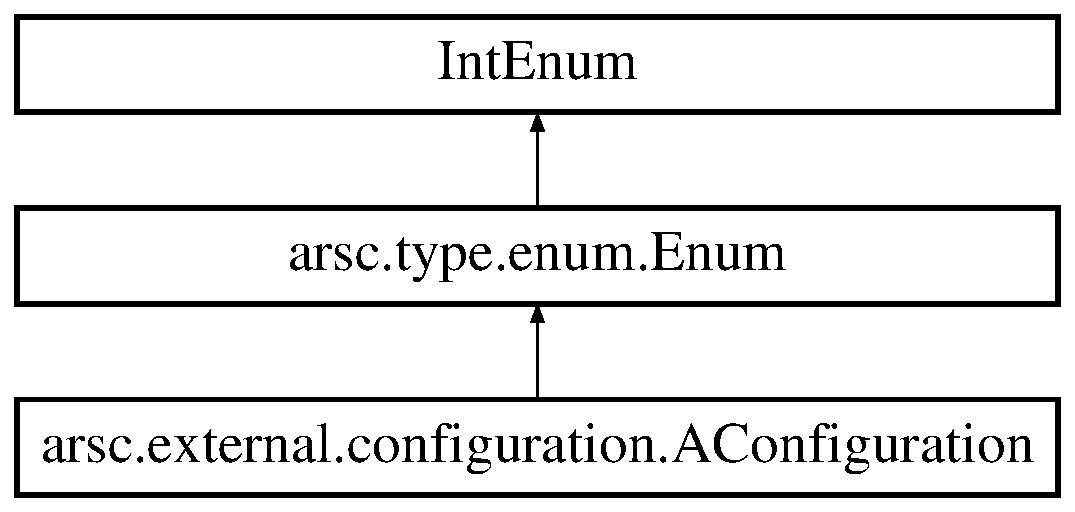
\includegraphics[height=3.000000cm]{classarsc_1_1external_1_1configuration_1_1AConfiguration}
\end{center}
\end{figure}
\subsection*{Static Public Attributes}
\begin{DoxyCompactItemize}
\item 
\mbox{\Hypertarget{classarsc_1_1external_1_1configuration_1_1AConfiguration_a06cf64f40e366782bc7d2fb1e10ddc76}\label{classarsc_1_1external_1_1configuration_1_1AConfiguration_a06cf64f40e366782bc7d2fb1e10ddc76}} 
int {\bfseries A\+C\+O\+N\+F\+I\+G\+U\+R\+A\+T\+I\+O\+N\+\_\+\+O\+R\+I\+E\+N\+T\+A\+T\+I\+O\+N\+\_\+\+A\+NY} = 0x0000
\item 
\mbox{\Hypertarget{classarsc_1_1external_1_1configuration_1_1AConfiguration_aee51ab8c375d82efa91b06510c4f39bb}\label{classarsc_1_1external_1_1configuration_1_1AConfiguration_aee51ab8c375d82efa91b06510c4f39bb}} 
int {\bfseries A\+C\+O\+N\+F\+I\+G\+U\+R\+A\+T\+I\+O\+N\+\_\+\+O\+R\+I\+E\+N\+T\+A\+T\+I\+O\+N\+\_\+\+P\+O\+RT} = 0x0001
\item 
\mbox{\Hypertarget{classarsc_1_1external_1_1configuration_1_1AConfiguration_a211d6f8110776575fb805e28025226cc}\label{classarsc_1_1external_1_1configuration_1_1AConfiguration_a211d6f8110776575fb805e28025226cc}} 
int {\bfseries A\+C\+O\+N\+F\+I\+G\+U\+R\+A\+T\+I\+O\+N\+\_\+\+O\+R\+I\+E\+N\+T\+A\+T\+I\+O\+N\+\_\+\+L\+A\+ND} = 0x0002
\item 
\mbox{\Hypertarget{classarsc_1_1external_1_1configuration_1_1AConfiguration_abaa3441f7795510f00339f19c89e0628}\label{classarsc_1_1external_1_1configuration_1_1AConfiguration_abaa3441f7795510f00339f19c89e0628}} 
int {\bfseries A\+C\+O\+N\+F\+I\+G\+U\+R\+A\+T\+I\+O\+N\+\_\+\+O\+R\+I\+E\+N\+T\+A\+T\+I\+O\+N\+\_\+\+S\+Q\+U\+A\+RE} = 0x0003
\item 
\mbox{\Hypertarget{classarsc_1_1external_1_1configuration_1_1AConfiguration_a040337807465fa6565970fcc3cfff351}\label{classarsc_1_1external_1_1configuration_1_1AConfiguration_a040337807465fa6565970fcc3cfff351}} 
int {\bfseries A\+C\+O\+N\+F\+I\+G\+U\+R\+A\+T\+I\+O\+N\+\_\+\+T\+O\+U\+C\+H\+S\+C\+R\+E\+E\+N\+\_\+\+A\+NY} = 0x0000
\item 
\mbox{\Hypertarget{classarsc_1_1external_1_1configuration_1_1AConfiguration_a352cf08b07ddb3d6d2c1031eb3439ca2}\label{classarsc_1_1external_1_1configuration_1_1AConfiguration_a352cf08b07ddb3d6d2c1031eb3439ca2}} 
int {\bfseries A\+C\+O\+N\+F\+I\+G\+U\+R\+A\+T\+I\+O\+N\+\_\+\+T\+O\+U\+C\+H\+S\+C\+R\+E\+E\+N\+\_\+\+N\+O\+T\+O\+U\+CH} = 0x0001
\item 
\mbox{\Hypertarget{classarsc_1_1external_1_1configuration_1_1AConfiguration_ab784ce4d21e17e5a2414877096336990}\label{classarsc_1_1external_1_1configuration_1_1AConfiguration_ab784ce4d21e17e5a2414877096336990}} 
int {\bfseries A\+C\+O\+N\+F\+I\+G\+U\+R\+A\+T\+I\+O\+N\+\_\+\+T\+O\+U\+C\+H\+S\+C\+R\+E\+E\+N\+\_\+\+S\+T\+Y\+L\+US} = 0x0002
\item 
\mbox{\Hypertarget{classarsc_1_1external_1_1configuration_1_1AConfiguration_a693cd5bcf845730db0d1a15df39c61bb}\label{classarsc_1_1external_1_1configuration_1_1AConfiguration_a693cd5bcf845730db0d1a15df39c61bb}} 
int {\bfseries A\+C\+O\+N\+F\+I\+G\+U\+R\+A\+T\+I\+O\+N\+\_\+\+T\+O\+U\+C\+H\+S\+C\+R\+E\+E\+N\+\_\+\+F\+I\+N\+G\+ER} = 0x0003
\item 
\mbox{\Hypertarget{classarsc_1_1external_1_1configuration_1_1AConfiguration_a95cef07ba739b109cf6c2b8665bab27f}\label{classarsc_1_1external_1_1configuration_1_1AConfiguration_a95cef07ba739b109cf6c2b8665bab27f}} 
int {\bfseries A\+C\+O\+N\+F\+I\+G\+U\+R\+A\+T\+I\+O\+N\+\_\+\+D\+E\+N\+S\+I\+T\+Y\+\_\+\+D\+E\+F\+A\+U\+LT} = 0
\item 
\mbox{\Hypertarget{classarsc_1_1external_1_1configuration_1_1AConfiguration_a8ac42547b7b2555ca20491807ee42c31}\label{classarsc_1_1external_1_1configuration_1_1AConfiguration_a8ac42547b7b2555ca20491807ee42c31}} 
int {\bfseries A\+C\+O\+N\+F\+I\+G\+U\+R\+A\+T\+I\+O\+N\+\_\+\+D\+E\+N\+S\+I\+T\+Y\+\_\+\+L\+OW} = 120
\item 
\mbox{\Hypertarget{classarsc_1_1external_1_1configuration_1_1AConfiguration_ad3501bab2a97d75235ce693380ef8b6d}\label{classarsc_1_1external_1_1configuration_1_1AConfiguration_ad3501bab2a97d75235ce693380ef8b6d}} 
int {\bfseries A\+C\+O\+N\+F\+I\+G\+U\+R\+A\+T\+I\+O\+N\+\_\+\+D\+E\+N\+S\+I\+T\+Y\+\_\+\+M\+E\+D\+I\+UM} = 160
\item 
\mbox{\Hypertarget{classarsc_1_1external_1_1configuration_1_1AConfiguration_ad843d4beecc740a8a02f78be0dbe9945}\label{classarsc_1_1external_1_1configuration_1_1AConfiguration_ad843d4beecc740a8a02f78be0dbe9945}} 
int {\bfseries A\+C\+O\+N\+F\+I\+G\+U\+R\+A\+T\+I\+O\+N\+\_\+\+D\+E\+N\+S\+I\+T\+Y\+\_\+\+TV} = 213
\item 
\mbox{\Hypertarget{classarsc_1_1external_1_1configuration_1_1AConfiguration_a70a96faf0e512bdee2270936af770e0b}\label{classarsc_1_1external_1_1configuration_1_1AConfiguration_a70a96faf0e512bdee2270936af770e0b}} 
int {\bfseries A\+C\+O\+N\+F\+I\+G\+U\+R\+A\+T\+I\+O\+N\+\_\+\+D\+E\+N\+S\+I\+T\+Y\+\_\+\+H\+I\+GH} = 240
\item 
\mbox{\Hypertarget{classarsc_1_1external_1_1configuration_1_1AConfiguration_abc197548e39f16903c3712071f0f5846}\label{classarsc_1_1external_1_1configuration_1_1AConfiguration_abc197548e39f16903c3712071f0f5846}} 
int {\bfseries A\+C\+O\+N\+F\+I\+G\+U\+R\+A\+T\+I\+O\+N\+\_\+\+D\+E\+N\+S\+I\+T\+Y\+\_\+\+X\+H\+I\+GH} = 320
\item 
\mbox{\Hypertarget{classarsc_1_1external_1_1configuration_1_1AConfiguration_ab707bda763e1ecdb9233af74ba8a62ce}\label{classarsc_1_1external_1_1configuration_1_1AConfiguration_ab707bda763e1ecdb9233af74ba8a62ce}} 
int {\bfseries A\+C\+O\+N\+F\+I\+G\+U\+R\+A\+T\+I\+O\+N\+\_\+\+D\+E\+N\+S\+I\+T\+Y\+\_\+\+X\+X\+H\+I\+GH} = 480
\item 
\mbox{\Hypertarget{classarsc_1_1external_1_1configuration_1_1AConfiguration_a1f1040a226d3ba0bf8bbc8781177f109}\label{classarsc_1_1external_1_1configuration_1_1AConfiguration_a1f1040a226d3ba0bf8bbc8781177f109}} 
int {\bfseries A\+C\+O\+N\+F\+I\+G\+U\+R\+A\+T\+I\+O\+N\+\_\+\+D\+E\+N\+S\+I\+T\+Y\+\_\+\+X\+X\+X\+H\+I\+GH} = 640
\item 
\mbox{\Hypertarget{classarsc_1_1external_1_1configuration_1_1AConfiguration_ac8887c487fb1d0b842f34dbf399e3fa4}\label{classarsc_1_1external_1_1configuration_1_1AConfiguration_ac8887c487fb1d0b842f34dbf399e3fa4}} 
int {\bfseries A\+C\+O\+N\+F\+I\+G\+U\+R\+A\+T\+I\+O\+N\+\_\+\+D\+E\+N\+S\+I\+T\+Y\+\_\+\+A\+NY} = 0xfffe
\item 
\mbox{\Hypertarget{classarsc_1_1external_1_1configuration_1_1AConfiguration_a75c6bb57ef04f7b55f59a263b7f65fbc}\label{classarsc_1_1external_1_1configuration_1_1AConfiguration_a75c6bb57ef04f7b55f59a263b7f65fbc}} 
int {\bfseries A\+C\+O\+N\+F\+I\+G\+U\+R\+A\+T\+I\+O\+N\+\_\+\+D\+E\+N\+S\+I\+T\+Y\+\_\+\+N\+O\+NE} = 0xffff
\item 
\mbox{\Hypertarget{classarsc_1_1external_1_1configuration_1_1AConfiguration_ae7d2c87597d98f074bd2fe9d0673416a}\label{classarsc_1_1external_1_1configuration_1_1AConfiguration_ae7d2c87597d98f074bd2fe9d0673416a}} 
int {\bfseries A\+C\+O\+N\+F\+I\+G\+U\+R\+A\+T\+I\+O\+N\+\_\+\+K\+E\+Y\+B\+O\+A\+R\+D\+\_\+\+A\+NY} = 0x0000
\item 
\mbox{\Hypertarget{classarsc_1_1external_1_1configuration_1_1AConfiguration_a830707f280cca35f61370cc234208fb5}\label{classarsc_1_1external_1_1configuration_1_1AConfiguration_a830707f280cca35f61370cc234208fb5}} 
int {\bfseries A\+C\+O\+N\+F\+I\+G\+U\+R\+A\+T\+I\+O\+N\+\_\+\+K\+E\+Y\+B\+O\+A\+R\+D\+\_\+\+N\+O\+K\+E\+YS} = 0x0001
\item 
\mbox{\Hypertarget{classarsc_1_1external_1_1configuration_1_1AConfiguration_ae48c1d225f51e5b7f59cb26ab2c97bf5}\label{classarsc_1_1external_1_1configuration_1_1AConfiguration_ae48c1d225f51e5b7f59cb26ab2c97bf5}} 
int {\bfseries A\+C\+O\+N\+F\+I\+G\+U\+R\+A\+T\+I\+O\+N\+\_\+\+K\+E\+Y\+B\+O\+A\+R\+D\+\_\+\+Q\+W\+E\+R\+TY} = 0x0002
\item 
\mbox{\Hypertarget{classarsc_1_1external_1_1configuration_1_1AConfiguration_aa15f9a019915e4cf021eb0381fa0cf80}\label{classarsc_1_1external_1_1configuration_1_1AConfiguration_aa15f9a019915e4cf021eb0381fa0cf80}} 
int {\bfseries A\+C\+O\+N\+F\+I\+G\+U\+R\+A\+T\+I\+O\+N\+\_\+\+K\+E\+Y\+B\+O\+A\+R\+D\+\_\+12\+K\+EY} = 0x0003
\item 
\mbox{\Hypertarget{classarsc_1_1external_1_1configuration_1_1AConfiguration_a8c35f29296bda2158ada62634b8ec783}\label{classarsc_1_1external_1_1configuration_1_1AConfiguration_a8c35f29296bda2158ada62634b8ec783}} 
int {\bfseries A\+C\+O\+N\+F\+I\+G\+U\+R\+A\+T\+I\+O\+N\+\_\+\+N\+A\+V\+I\+G\+A\+T\+I\+O\+N\+\_\+\+A\+NY} = 0x0000
\item 
\mbox{\Hypertarget{classarsc_1_1external_1_1configuration_1_1AConfiguration_a1c8c6bec2f6323e738df62bdbed27642}\label{classarsc_1_1external_1_1configuration_1_1AConfiguration_a1c8c6bec2f6323e738df62bdbed27642}} 
int {\bfseries A\+C\+O\+N\+F\+I\+G\+U\+R\+A\+T\+I\+O\+N\+\_\+\+N\+A\+V\+I\+G\+A\+T\+I\+O\+N\+\_\+\+N\+O\+N\+AV} = 0x0001
\item 
\mbox{\Hypertarget{classarsc_1_1external_1_1configuration_1_1AConfiguration_a964e9c9094312e54777f43d8eeec71f4}\label{classarsc_1_1external_1_1configuration_1_1AConfiguration_a964e9c9094312e54777f43d8eeec71f4}} 
int {\bfseries A\+C\+O\+N\+F\+I\+G\+U\+R\+A\+T\+I\+O\+N\+\_\+\+N\+A\+V\+I\+G\+A\+T\+I\+O\+N\+\_\+\+D\+P\+AD} = 0x0002
\item 
\mbox{\Hypertarget{classarsc_1_1external_1_1configuration_1_1AConfiguration_a44634018742f3b6cf66a1c624084870d}\label{classarsc_1_1external_1_1configuration_1_1AConfiguration_a44634018742f3b6cf66a1c624084870d}} 
int {\bfseries A\+C\+O\+N\+F\+I\+G\+U\+R\+A\+T\+I\+O\+N\+\_\+\+N\+A\+V\+I\+G\+A\+T\+I\+O\+N\+\_\+\+T\+R\+A\+C\+K\+B\+A\+LL} = 0x0003
\item 
\mbox{\Hypertarget{classarsc_1_1external_1_1configuration_1_1AConfiguration_a4e375d1ffe0b3ab064b102b442fc5407}\label{classarsc_1_1external_1_1configuration_1_1AConfiguration_a4e375d1ffe0b3ab064b102b442fc5407}} 
int {\bfseries A\+C\+O\+N\+F\+I\+G\+U\+R\+A\+T\+I\+O\+N\+\_\+\+N\+A\+V\+I\+G\+A\+T\+I\+O\+N\+\_\+\+W\+H\+E\+EL} = 0x0004
\item 
\mbox{\Hypertarget{classarsc_1_1external_1_1configuration_1_1AConfiguration_a091c3f7d0cc535ca5eae5521386dae73}\label{classarsc_1_1external_1_1configuration_1_1AConfiguration_a091c3f7d0cc535ca5eae5521386dae73}} 
int {\bfseries A\+C\+O\+N\+F\+I\+G\+U\+R\+A\+T\+I\+O\+N\+\_\+\+K\+E\+Y\+S\+H\+I\+D\+D\+E\+N\+\_\+\+A\+NY} = 0x0000
\item 
\mbox{\Hypertarget{classarsc_1_1external_1_1configuration_1_1AConfiguration_a85d142bbb5b78ae7c76fc3a250b44109}\label{classarsc_1_1external_1_1configuration_1_1AConfiguration_a85d142bbb5b78ae7c76fc3a250b44109}} 
int {\bfseries A\+C\+O\+N\+F\+I\+G\+U\+R\+A\+T\+I\+O\+N\+\_\+\+K\+E\+Y\+S\+H\+I\+D\+D\+E\+N\+\_\+\+NO} = 0x0001
\item 
\mbox{\Hypertarget{classarsc_1_1external_1_1configuration_1_1AConfiguration_a75e2fcd1891f6846bbc7634e1c8ca052}\label{classarsc_1_1external_1_1configuration_1_1AConfiguration_a75e2fcd1891f6846bbc7634e1c8ca052}} 
int {\bfseries A\+C\+O\+N\+F\+I\+G\+U\+R\+A\+T\+I\+O\+N\+\_\+\+K\+E\+Y\+S\+H\+I\+D\+D\+E\+N\+\_\+\+Y\+ES} = 0x0002
\item 
\mbox{\Hypertarget{classarsc_1_1external_1_1configuration_1_1AConfiguration_aa20ce318897cbbb140e739cc20be06f6}\label{classarsc_1_1external_1_1configuration_1_1AConfiguration_aa20ce318897cbbb140e739cc20be06f6}} 
int {\bfseries A\+C\+O\+N\+F\+I\+G\+U\+R\+A\+T\+I\+O\+N\+\_\+\+K\+E\+Y\+S\+H\+I\+D\+D\+E\+N\+\_\+\+S\+O\+FT} = 0x0003
\item 
\mbox{\Hypertarget{classarsc_1_1external_1_1configuration_1_1AConfiguration_a216be2de4fe4cb28eb42807e203ee79d}\label{classarsc_1_1external_1_1configuration_1_1AConfiguration_a216be2de4fe4cb28eb42807e203ee79d}} 
int {\bfseries A\+C\+O\+N\+F\+I\+G\+U\+R\+A\+T\+I\+O\+N\+\_\+\+N\+A\+V\+H\+I\+D\+D\+E\+N\+\_\+\+A\+NY} = 0x0000
\item 
\mbox{\Hypertarget{classarsc_1_1external_1_1configuration_1_1AConfiguration_a552aac9a6444a05af67a692eaa4157f9}\label{classarsc_1_1external_1_1configuration_1_1AConfiguration_a552aac9a6444a05af67a692eaa4157f9}} 
int {\bfseries A\+C\+O\+N\+F\+I\+G\+U\+R\+A\+T\+I\+O\+N\+\_\+\+N\+A\+V\+H\+I\+D\+D\+E\+N\+\_\+\+NO} = 0x0001
\item 
\mbox{\Hypertarget{classarsc_1_1external_1_1configuration_1_1AConfiguration_a73cdf1ee3e10ba105bc57ac723d65fa9}\label{classarsc_1_1external_1_1configuration_1_1AConfiguration_a73cdf1ee3e10ba105bc57ac723d65fa9}} 
int {\bfseries A\+C\+O\+N\+F\+I\+G\+U\+R\+A\+T\+I\+O\+N\+\_\+\+N\+A\+V\+H\+I\+D\+D\+E\+N\+\_\+\+Y\+ES} = 0x0002
\item 
\mbox{\Hypertarget{classarsc_1_1external_1_1configuration_1_1AConfiguration_a7b1eb75d06ab3be669a6884ea521c4c6}\label{classarsc_1_1external_1_1configuration_1_1AConfiguration_a7b1eb75d06ab3be669a6884ea521c4c6}} 
int {\bfseries A\+C\+O\+N\+F\+I\+G\+U\+R\+A\+T\+I\+O\+N\+\_\+\+S\+C\+R\+E\+E\+N\+S\+I\+Z\+E\+\_\+\+A\+NY} = 0x00
\item 
\mbox{\Hypertarget{classarsc_1_1external_1_1configuration_1_1AConfiguration_ad5a21db2068577ae93813464be3a803c}\label{classarsc_1_1external_1_1configuration_1_1AConfiguration_ad5a21db2068577ae93813464be3a803c}} 
int {\bfseries A\+C\+O\+N\+F\+I\+G\+U\+R\+A\+T\+I\+O\+N\+\_\+\+S\+C\+R\+E\+E\+N\+S\+I\+Z\+E\+\_\+\+S\+M\+A\+LL} = 0x01
\item 
\mbox{\Hypertarget{classarsc_1_1external_1_1configuration_1_1AConfiguration_adb62b70aaef566ca7ea8393c22d1bd21}\label{classarsc_1_1external_1_1configuration_1_1AConfiguration_adb62b70aaef566ca7ea8393c22d1bd21}} 
int {\bfseries A\+C\+O\+N\+F\+I\+G\+U\+R\+A\+T\+I\+O\+N\+\_\+\+S\+C\+R\+E\+E\+N\+S\+I\+Z\+E\+\_\+\+N\+O\+R\+M\+AL} = 0x02
\item 
\mbox{\Hypertarget{classarsc_1_1external_1_1configuration_1_1AConfiguration_a7ee98551d0be89d5eadde142b5ff48bc}\label{classarsc_1_1external_1_1configuration_1_1AConfiguration_a7ee98551d0be89d5eadde142b5ff48bc}} 
int {\bfseries A\+C\+O\+N\+F\+I\+G\+U\+R\+A\+T\+I\+O\+N\+\_\+\+S\+C\+R\+E\+E\+N\+S\+I\+Z\+E\+\_\+\+L\+A\+R\+GE} = 0x03
\item 
\mbox{\Hypertarget{classarsc_1_1external_1_1configuration_1_1AConfiguration_af28ba3f4dcb70300425fd318eb1e4bd0}\label{classarsc_1_1external_1_1configuration_1_1AConfiguration_af28ba3f4dcb70300425fd318eb1e4bd0}} 
int {\bfseries A\+C\+O\+N\+F\+I\+G\+U\+R\+A\+T\+I\+O\+N\+\_\+\+S\+C\+R\+E\+E\+N\+S\+I\+Z\+E\+\_\+\+X\+L\+A\+R\+GE} = 0x04
\item 
\mbox{\Hypertarget{classarsc_1_1external_1_1configuration_1_1AConfiguration_a15c2737d51bbc71a3e47231021df532f}\label{classarsc_1_1external_1_1configuration_1_1AConfiguration_a15c2737d51bbc71a3e47231021df532f}} 
int {\bfseries A\+C\+O\+N\+F\+I\+G\+U\+R\+A\+T\+I\+O\+N\+\_\+\+S\+C\+R\+E\+E\+N\+L\+O\+N\+G\+\_\+\+A\+NY} = 0x00
\item 
\mbox{\Hypertarget{classarsc_1_1external_1_1configuration_1_1AConfiguration_a797c6699ed5b4435481d7e30d72493b2}\label{classarsc_1_1external_1_1configuration_1_1AConfiguration_a797c6699ed5b4435481d7e30d72493b2}} 
int {\bfseries A\+C\+O\+N\+F\+I\+G\+U\+R\+A\+T\+I\+O\+N\+\_\+\+S\+C\+R\+E\+E\+N\+L\+O\+N\+G\+\_\+\+NO} = 0x1
\item 
\mbox{\Hypertarget{classarsc_1_1external_1_1configuration_1_1AConfiguration_a7c846a44cc07725fdcae432b0c8f0a46}\label{classarsc_1_1external_1_1configuration_1_1AConfiguration_a7c846a44cc07725fdcae432b0c8f0a46}} 
int {\bfseries A\+C\+O\+N\+F\+I\+G\+U\+R\+A\+T\+I\+O\+N\+\_\+\+S\+C\+R\+E\+E\+N\+L\+O\+N\+G\+\_\+\+Y\+ES} = 0x2
\item 
\mbox{\Hypertarget{classarsc_1_1external_1_1configuration_1_1AConfiguration_a1065d2f7c006d849092340ba0c7fac77}\label{classarsc_1_1external_1_1configuration_1_1AConfiguration_a1065d2f7c006d849092340ba0c7fac77}} 
int {\bfseries A\+C\+O\+N\+F\+I\+G\+U\+R\+A\+T\+I\+O\+N\+\_\+\+S\+C\+R\+E\+E\+N\+R\+O\+U\+N\+D\+\_\+\+A\+NY} = 0x00
\item 
\mbox{\Hypertarget{classarsc_1_1external_1_1configuration_1_1AConfiguration_a532ff10e50de959a572a2872bcc9e587}\label{classarsc_1_1external_1_1configuration_1_1AConfiguration_a532ff10e50de959a572a2872bcc9e587}} 
int {\bfseries A\+C\+O\+N\+F\+I\+G\+U\+R\+A\+T\+I\+O\+N\+\_\+\+S\+C\+R\+E\+E\+N\+R\+O\+U\+N\+D\+\_\+\+NO} = 0x1
\item 
\mbox{\Hypertarget{classarsc_1_1external_1_1configuration_1_1AConfiguration_ab3d3ac5941ec4a4d5af3c1952302c561}\label{classarsc_1_1external_1_1configuration_1_1AConfiguration_ab3d3ac5941ec4a4d5af3c1952302c561}} 
int {\bfseries A\+C\+O\+N\+F\+I\+G\+U\+R\+A\+T\+I\+O\+N\+\_\+\+S\+C\+R\+E\+E\+N\+R\+O\+U\+N\+D\+\_\+\+Y\+ES} = 0x2
\item 
\mbox{\Hypertarget{classarsc_1_1external_1_1configuration_1_1AConfiguration_a0ede7b40c8f16c86b2cfa99a74b1b102}\label{classarsc_1_1external_1_1configuration_1_1AConfiguration_a0ede7b40c8f16c86b2cfa99a74b1b102}} 
int {\bfseries A\+C\+O\+N\+F\+I\+G\+U\+R\+A\+T\+I\+O\+N\+\_\+\+W\+I\+D\+E\+\_\+\+C\+O\+L\+O\+R\+\_\+\+G\+A\+M\+U\+T\+\_\+\+A\+NY} = 0x00
\item 
\mbox{\Hypertarget{classarsc_1_1external_1_1configuration_1_1AConfiguration_a6abc1044c93f136a17e76f42f5dcfd96}\label{classarsc_1_1external_1_1configuration_1_1AConfiguration_a6abc1044c93f136a17e76f42f5dcfd96}} 
int {\bfseries A\+C\+O\+N\+F\+I\+G\+U\+R\+A\+T\+I\+O\+N\+\_\+\+W\+I\+D\+E\+\_\+\+C\+O\+L\+O\+R\+\_\+\+G\+A\+M\+U\+T\+\_\+\+NO} = 0x1
\item 
\mbox{\Hypertarget{classarsc_1_1external_1_1configuration_1_1AConfiguration_a2e04f813348c2310b52ff403a4208f2b}\label{classarsc_1_1external_1_1configuration_1_1AConfiguration_a2e04f813348c2310b52ff403a4208f2b}} 
int {\bfseries A\+C\+O\+N\+F\+I\+G\+U\+R\+A\+T\+I\+O\+N\+\_\+\+W\+I\+D\+E\+\_\+\+C\+O\+L\+O\+R\+\_\+\+G\+A\+M\+U\+T\+\_\+\+Y\+ES} = 0x2
\item 
\mbox{\Hypertarget{classarsc_1_1external_1_1configuration_1_1AConfiguration_a3347af03ff6b4a77a21ebd56c778b992}\label{classarsc_1_1external_1_1configuration_1_1AConfiguration_a3347af03ff6b4a77a21ebd56c778b992}} 
int {\bfseries A\+C\+O\+N\+F\+I\+G\+U\+R\+A\+T\+I\+O\+N\+\_\+\+H\+D\+R\+\_\+\+A\+NY} = 0x00
\item 
\mbox{\Hypertarget{classarsc_1_1external_1_1configuration_1_1AConfiguration_af8da9be81d4967388c45975a797b30a7}\label{classarsc_1_1external_1_1configuration_1_1AConfiguration_af8da9be81d4967388c45975a797b30a7}} 
int {\bfseries A\+C\+O\+N\+F\+I\+G\+U\+R\+A\+T\+I\+O\+N\+\_\+\+H\+D\+R\+\_\+\+NO} = 0x1
\item 
\mbox{\Hypertarget{classarsc_1_1external_1_1configuration_1_1AConfiguration_ab06797e45fb5fc6bac7cf0b7299a34ac}\label{classarsc_1_1external_1_1configuration_1_1AConfiguration_ab06797e45fb5fc6bac7cf0b7299a34ac}} 
int {\bfseries A\+C\+O\+N\+F\+I\+G\+U\+R\+A\+T\+I\+O\+N\+\_\+\+H\+D\+R\+\_\+\+Y\+ES} = 0x2
\item 
\mbox{\Hypertarget{classarsc_1_1external_1_1configuration_1_1AConfiguration_af0e501418b0fa7b7f606648d06e54b48}\label{classarsc_1_1external_1_1configuration_1_1AConfiguration_af0e501418b0fa7b7f606648d06e54b48}} 
int {\bfseries A\+C\+O\+N\+F\+I\+G\+U\+R\+A\+T\+I\+O\+N\+\_\+\+U\+I\+\_\+\+M\+O\+D\+E\+\_\+\+T\+Y\+P\+E\+\_\+\+A\+NY} = 0x00
\item 
\mbox{\Hypertarget{classarsc_1_1external_1_1configuration_1_1AConfiguration_ac6cf6e311a014018ecc1b8fe3c523ead}\label{classarsc_1_1external_1_1configuration_1_1AConfiguration_ac6cf6e311a014018ecc1b8fe3c523ead}} 
int {\bfseries A\+C\+O\+N\+F\+I\+G\+U\+R\+A\+T\+I\+O\+N\+\_\+\+U\+I\+\_\+\+M\+O\+D\+E\+\_\+\+T\+Y\+P\+E\+\_\+\+N\+O\+R\+M\+AL} = 0x01
\item 
\mbox{\Hypertarget{classarsc_1_1external_1_1configuration_1_1AConfiguration_a0f1fa67e2ac1c2a9ff803c4f9ac79f27}\label{classarsc_1_1external_1_1configuration_1_1AConfiguration_a0f1fa67e2ac1c2a9ff803c4f9ac79f27}} 
int {\bfseries A\+C\+O\+N\+F\+I\+G\+U\+R\+A\+T\+I\+O\+N\+\_\+\+U\+I\+\_\+\+M\+O\+D\+E\+\_\+\+T\+Y\+P\+E\+\_\+\+D\+E\+SK} = 0x02
\item 
\mbox{\Hypertarget{classarsc_1_1external_1_1configuration_1_1AConfiguration_aa56eaa0ac49572eaaaf7ebb492af5eaf}\label{classarsc_1_1external_1_1configuration_1_1AConfiguration_aa56eaa0ac49572eaaaf7ebb492af5eaf}} 
int {\bfseries A\+C\+O\+N\+F\+I\+G\+U\+R\+A\+T\+I\+O\+N\+\_\+\+U\+I\+\_\+\+M\+O\+D\+E\+\_\+\+T\+Y\+P\+E\+\_\+\+C\+AR} = 0x03
\item 
\mbox{\Hypertarget{classarsc_1_1external_1_1configuration_1_1AConfiguration_aa9c040a1ce23cc3ab3b240a73443ca68}\label{classarsc_1_1external_1_1configuration_1_1AConfiguration_aa9c040a1ce23cc3ab3b240a73443ca68}} 
int {\bfseries A\+C\+O\+N\+F\+I\+G\+U\+R\+A\+T\+I\+O\+N\+\_\+\+U\+I\+\_\+\+M\+O\+D\+E\+\_\+\+T\+Y\+P\+E\+\_\+\+T\+E\+L\+E\+V\+I\+S\+I\+ON} = 0x04
\item 
\mbox{\Hypertarget{classarsc_1_1external_1_1configuration_1_1AConfiguration_a11ed0b274706545587b6e78bd3d1ee2b}\label{classarsc_1_1external_1_1configuration_1_1AConfiguration_a11ed0b274706545587b6e78bd3d1ee2b}} 
int {\bfseries A\+C\+O\+N\+F\+I\+G\+U\+R\+A\+T\+I\+O\+N\+\_\+\+U\+I\+\_\+\+M\+O\+D\+E\+\_\+\+T\+Y\+P\+E\+\_\+\+A\+P\+P\+L\+I\+A\+N\+CE} = 0x05
\item 
\mbox{\Hypertarget{classarsc_1_1external_1_1configuration_1_1AConfiguration_abe7d7ecd5071491c8e0a8e1297b7e8eb}\label{classarsc_1_1external_1_1configuration_1_1AConfiguration_abe7d7ecd5071491c8e0a8e1297b7e8eb}} 
int {\bfseries A\+C\+O\+N\+F\+I\+G\+U\+R\+A\+T\+I\+O\+N\+\_\+\+U\+I\+\_\+\+M\+O\+D\+E\+\_\+\+T\+Y\+P\+E\+\_\+\+W\+A\+T\+CH} = 0x06
\item 
\mbox{\Hypertarget{classarsc_1_1external_1_1configuration_1_1AConfiguration_a0e7951479802623545691abd4117c920}\label{classarsc_1_1external_1_1configuration_1_1AConfiguration_a0e7951479802623545691abd4117c920}} 
int {\bfseries A\+C\+O\+N\+F\+I\+G\+U\+R\+A\+T\+I\+O\+N\+\_\+\+U\+I\+\_\+\+M\+O\+D\+E\+\_\+\+T\+Y\+P\+E\+\_\+\+V\+R\+\_\+\+H\+E\+A\+D\+S\+ET} = 0x07
\item 
\mbox{\Hypertarget{classarsc_1_1external_1_1configuration_1_1AConfiguration_a7460ba14b25de467e1c12508c0d2c1d9}\label{classarsc_1_1external_1_1configuration_1_1AConfiguration_a7460ba14b25de467e1c12508c0d2c1d9}} 
int {\bfseries A\+C\+O\+N\+F\+I\+G\+U\+R\+A\+T\+I\+O\+N\+\_\+\+U\+I\+\_\+\+M\+O\+D\+E\+\_\+\+N\+I\+G\+H\+T\+\_\+\+A\+NY} = 0x00
\item 
\mbox{\Hypertarget{classarsc_1_1external_1_1configuration_1_1AConfiguration_a1e60c6a7d57a129330b024ad7f2ddf8d}\label{classarsc_1_1external_1_1configuration_1_1AConfiguration_a1e60c6a7d57a129330b024ad7f2ddf8d}} 
int {\bfseries A\+C\+O\+N\+F\+I\+G\+U\+R\+A\+T\+I\+O\+N\+\_\+\+U\+I\+\_\+\+M\+O\+D\+E\+\_\+\+N\+I\+G\+H\+T\+\_\+\+NO} = 0x1
\item 
\mbox{\Hypertarget{classarsc_1_1external_1_1configuration_1_1AConfiguration_a0009054b99297ea4938f3cfe5fa18de9}\label{classarsc_1_1external_1_1configuration_1_1AConfiguration_a0009054b99297ea4938f3cfe5fa18de9}} 
int {\bfseries A\+C\+O\+N\+F\+I\+G\+U\+R\+A\+T\+I\+O\+N\+\_\+\+U\+I\+\_\+\+M\+O\+D\+E\+\_\+\+N\+I\+G\+H\+T\+\_\+\+Y\+ES} = 0x2
\item 
\mbox{\Hypertarget{classarsc_1_1external_1_1configuration_1_1AConfiguration_ab08ccc92d4ecf41c86c0e6d6b596f31f}\label{classarsc_1_1external_1_1configuration_1_1AConfiguration_ab08ccc92d4ecf41c86c0e6d6b596f31f}} 
int {\bfseries A\+C\+O\+N\+F\+I\+G\+U\+R\+A\+T\+I\+O\+N\+\_\+\+S\+C\+R\+E\+E\+N\+\_\+\+W\+I\+D\+T\+H\+\_\+\+D\+P\+\_\+\+A\+NY} = 0x0000
\item 
\mbox{\Hypertarget{classarsc_1_1external_1_1configuration_1_1AConfiguration_aa23b4026b9f1012ec5d3647ca5761cb4}\label{classarsc_1_1external_1_1configuration_1_1AConfiguration_aa23b4026b9f1012ec5d3647ca5761cb4}} 
int {\bfseries A\+C\+O\+N\+F\+I\+G\+U\+R\+A\+T\+I\+O\+N\+\_\+\+S\+C\+R\+E\+E\+N\+\_\+\+H\+E\+I\+G\+H\+T\+\_\+\+D\+P\+\_\+\+A\+NY} = 0x0000
\item 
\mbox{\Hypertarget{classarsc_1_1external_1_1configuration_1_1AConfiguration_acfa6735023caa0d52292d1228f589ea7}\label{classarsc_1_1external_1_1configuration_1_1AConfiguration_acfa6735023caa0d52292d1228f589ea7}} 
int {\bfseries A\+C\+O\+N\+F\+I\+G\+U\+R\+A\+T\+I\+O\+N\+\_\+\+S\+M\+A\+L\+L\+E\+S\+T\+\_\+\+S\+C\+R\+E\+E\+N\+\_\+\+W\+I\+D\+T\+H\+\_\+\+D\+P\+\_\+\+A\+NY} = 0x0000
\item 
\mbox{\Hypertarget{classarsc_1_1external_1_1configuration_1_1AConfiguration_a46e622e0316d8f38c0f1799ec098ebbd}\label{classarsc_1_1external_1_1configuration_1_1AConfiguration_a46e622e0316d8f38c0f1799ec098ebbd}} 
int {\bfseries A\+C\+O\+N\+F\+I\+G\+U\+R\+A\+T\+I\+O\+N\+\_\+\+L\+A\+Y\+O\+U\+T\+D\+I\+R\+\_\+\+A\+NY} = 0x00
\item 
\mbox{\Hypertarget{classarsc_1_1external_1_1configuration_1_1AConfiguration_ac5c6e35199260ab6648ff4aac17e5b78}\label{classarsc_1_1external_1_1configuration_1_1AConfiguration_ac5c6e35199260ab6648ff4aac17e5b78}} 
int {\bfseries A\+C\+O\+N\+F\+I\+G\+U\+R\+A\+T\+I\+O\+N\+\_\+\+L\+A\+Y\+O\+U\+T\+D\+I\+R\+\_\+\+L\+TR} = 0x01
\item 
\mbox{\Hypertarget{classarsc_1_1external_1_1configuration_1_1AConfiguration_a669a5f79ce81e7e4691c051b80402cf3}\label{classarsc_1_1external_1_1configuration_1_1AConfiguration_a669a5f79ce81e7e4691c051b80402cf3}} 
int {\bfseries A\+C\+O\+N\+F\+I\+G\+U\+R\+A\+T\+I\+O\+N\+\_\+\+L\+A\+Y\+O\+U\+T\+D\+I\+R\+\_\+\+R\+TL} = 0x02
\item 
\mbox{\Hypertarget{classarsc_1_1external_1_1configuration_1_1AConfiguration_a96a475fed198a17eb2d5fc4fb6cdd7e8}\label{classarsc_1_1external_1_1configuration_1_1AConfiguration_a96a475fed198a17eb2d5fc4fb6cdd7e8}} 
int {\bfseries A\+C\+O\+N\+F\+I\+G\+U\+R\+A\+T\+I\+O\+N\+\_\+\+M\+CC} = 0x0001
\item 
\mbox{\Hypertarget{classarsc_1_1external_1_1configuration_1_1AConfiguration_a572376849e72b7bbaf276642684bdca1}\label{classarsc_1_1external_1_1configuration_1_1AConfiguration_a572376849e72b7bbaf276642684bdca1}} 
int {\bfseries A\+C\+O\+N\+F\+I\+G\+U\+R\+A\+T\+I\+O\+N\+\_\+\+M\+NC} = 0x0002
\item 
\mbox{\Hypertarget{classarsc_1_1external_1_1configuration_1_1AConfiguration_ad7f14a8ac225a77cff64f95e7093d505}\label{classarsc_1_1external_1_1configuration_1_1AConfiguration_ad7f14a8ac225a77cff64f95e7093d505}} 
int {\bfseries A\+C\+O\+N\+F\+I\+G\+U\+R\+A\+T\+I\+O\+N\+\_\+\+L\+O\+C\+A\+LE} = 0x0004
\item 
\mbox{\Hypertarget{classarsc_1_1external_1_1configuration_1_1AConfiguration_aec3725095c3b966aea3986ee9fc8f8cd}\label{classarsc_1_1external_1_1configuration_1_1AConfiguration_aec3725095c3b966aea3986ee9fc8f8cd}} 
int {\bfseries A\+C\+O\+N\+F\+I\+G\+U\+R\+A\+T\+I\+O\+N\+\_\+\+T\+O\+U\+C\+H\+S\+C\+R\+E\+EN} = 0x0008
\item 
\mbox{\Hypertarget{classarsc_1_1external_1_1configuration_1_1AConfiguration_ab9d7a330b94e10fa03340cd6810b2330}\label{classarsc_1_1external_1_1configuration_1_1AConfiguration_ab9d7a330b94e10fa03340cd6810b2330}} 
int {\bfseries A\+C\+O\+N\+F\+I\+G\+U\+R\+A\+T\+I\+O\+N\+\_\+\+K\+E\+Y\+B\+O\+A\+RD} = 0x0010
\item 
\mbox{\Hypertarget{classarsc_1_1external_1_1configuration_1_1AConfiguration_a3f49dd0ca1bf21edd42ef468443ce9ef}\label{classarsc_1_1external_1_1configuration_1_1AConfiguration_a3f49dd0ca1bf21edd42ef468443ce9ef}} 
int {\bfseries A\+C\+O\+N\+F\+I\+G\+U\+R\+A\+T\+I\+O\+N\+\_\+\+K\+E\+Y\+B\+O\+A\+R\+D\+\_\+\+H\+I\+D\+D\+EN} = 0x0020
\item 
\mbox{\Hypertarget{classarsc_1_1external_1_1configuration_1_1AConfiguration_a65bca76915a081497b5e491b31277c9f}\label{classarsc_1_1external_1_1configuration_1_1AConfiguration_a65bca76915a081497b5e491b31277c9f}} 
int {\bfseries A\+C\+O\+N\+F\+I\+G\+U\+R\+A\+T\+I\+O\+N\+\_\+\+N\+A\+V\+I\+G\+A\+T\+I\+ON} = 0x0040
\item 
\mbox{\Hypertarget{classarsc_1_1external_1_1configuration_1_1AConfiguration_ab14895c2903e6c356eed94de582febcd}\label{classarsc_1_1external_1_1configuration_1_1AConfiguration_ab14895c2903e6c356eed94de582febcd}} 
int {\bfseries A\+C\+O\+N\+F\+I\+G\+U\+R\+A\+T\+I\+O\+N\+\_\+\+O\+R\+I\+E\+N\+T\+A\+T\+I\+ON} = 0x0080
\item 
\mbox{\Hypertarget{classarsc_1_1external_1_1configuration_1_1AConfiguration_a63c2dac855d05e3e8e8cae9bc7ff2bbf}\label{classarsc_1_1external_1_1configuration_1_1AConfiguration_a63c2dac855d05e3e8e8cae9bc7ff2bbf}} 
int {\bfseries A\+C\+O\+N\+F\+I\+G\+U\+R\+A\+T\+I\+O\+N\+\_\+\+D\+E\+N\+S\+I\+TY} = 0x0100
\item 
\mbox{\Hypertarget{classarsc_1_1external_1_1configuration_1_1AConfiguration_a71d77e7a8dc79e3f7ff315747eec340d}\label{classarsc_1_1external_1_1configuration_1_1AConfiguration_a71d77e7a8dc79e3f7ff315747eec340d}} 
int {\bfseries A\+C\+O\+N\+F\+I\+G\+U\+R\+A\+T\+I\+O\+N\+\_\+\+S\+C\+R\+E\+E\+N\+\_\+\+S\+I\+ZE} = 0x0200
\item 
\mbox{\Hypertarget{classarsc_1_1external_1_1configuration_1_1AConfiguration_a7dfb451364d519fad9f36f95fcb14f98}\label{classarsc_1_1external_1_1configuration_1_1AConfiguration_a7dfb451364d519fad9f36f95fcb14f98}} 
int {\bfseries A\+C\+O\+N\+F\+I\+G\+U\+R\+A\+T\+I\+O\+N\+\_\+\+V\+E\+R\+S\+I\+ON} = 0x0400
\item 
\mbox{\Hypertarget{classarsc_1_1external_1_1configuration_1_1AConfiguration_adb2282dc170511fced1d30c184574a0c}\label{classarsc_1_1external_1_1configuration_1_1AConfiguration_adb2282dc170511fced1d30c184574a0c}} 
int {\bfseries A\+C\+O\+N\+F\+I\+G\+U\+R\+A\+T\+I\+O\+N\+\_\+\+S\+C\+R\+E\+E\+N\+\_\+\+L\+A\+Y\+O\+UT} = 0x0800
\item 
\mbox{\Hypertarget{classarsc_1_1external_1_1configuration_1_1AConfiguration_a3fba47fe7262715a737d2c39f85fa5f5}\label{classarsc_1_1external_1_1configuration_1_1AConfiguration_a3fba47fe7262715a737d2c39f85fa5f5}} 
int {\bfseries A\+C\+O\+N\+F\+I\+G\+U\+R\+A\+T\+I\+O\+N\+\_\+\+U\+I\+\_\+\+M\+O\+DE} = 0x1000
\item 
\mbox{\Hypertarget{classarsc_1_1external_1_1configuration_1_1AConfiguration_a1cf5edf4bbd1550329f55fa6306787a7}\label{classarsc_1_1external_1_1configuration_1_1AConfiguration_a1cf5edf4bbd1550329f55fa6306787a7}} 
int {\bfseries A\+C\+O\+N\+F\+I\+G\+U\+R\+A\+T\+I\+O\+N\+\_\+\+S\+M\+A\+L\+L\+E\+S\+T\+\_\+\+S\+C\+R\+E\+E\+N\+\_\+\+S\+I\+ZE} = 0x2000
\item 
\mbox{\Hypertarget{classarsc_1_1external_1_1configuration_1_1AConfiguration_aaaabadd26c5ce00b9594ddfa451499c2}\label{classarsc_1_1external_1_1configuration_1_1AConfiguration_aaaabadd26c5ce00b9594ddfa451499c2}} 
int {\bfseries A\+C\+O\+N\+F\+I\+G\+U\+R\+A\+T\+I\+O\+N\+\_\+\+L\+A\+Y\+O\+U\+T\+D\+IR} = 0x4000
\item 
\mbox{\Hypertarget{classarsc_1_1external_1_1configuration_1_1AConfiguration_a3d9fdb4ff9f6e46eb07732ea108accf3}\label{classarsc_1_1external_1_1configuration_1_1AConfiguration_a3d9fdb4ff9f6e46eb07732ea108accf3}} 
int {\bfseries A\+C\+O\+N\+F\+I\+G\+U\+R\+A\+T\+I\+O\+N\+\_\+\+S\+C\+R\+E\+E\+N\+\_\+\+R\+O\+U\+ND} = 0x8000
\item 
\mbox{\Hypertarget{classarsc_1_1external_1_1configuration_1_1AConfiguration_ac36d76a5570798eb212277588a064c0e}\label{classarsc_1_1external_1_1configuration_1_1AConfiguration_ac36d76a5570798eb212277588a064c0e}} 
int {\bfseries A\+C\+O\+N\+F\+I\+G\+U\+R\+A\+T\+I\+O\+N\+\_\+\+C\+O\+L\+O\+R\+\_\+\+M\+O\+DE} = 0x10000
\item 
\mbox{\Hypertarget{classarsc_1_1external_1_1configuration_1_1AConfiguration_abfb660865d88d4b4860cdd08566c329e}\label{classarsc_1_1external_1_1configuration_1_1AConfiguration_abfb660865d88d4b4860cdd08566c329e}} 
int {\bfseries A\+C\+O\+N\+F\+I\+G\+U\+R\+A\+T\+I\+O\+N\+\_\+\+M\+N\+C\+\_\+\+Z\+E\+RO} = 0xffff
\end{DoxyCompactItemize}
\subsection*{Additional Inherited Members}


The documentation for this class was generated from the following file\+:\begin{DoxyCompactItemize}
\item 
arsc/external/\mbox{\hyperlink{configuration_8py}{configuration.\+py}}\end{DoxyCompactItemize}

\hypertarget{classarsc_1_1exceptions_1_1ChunkHeaderWrongTypeException}{}\section{arsc.\+exceptions.\+Chunk\+Header\+Wrong\+Type\+Exception Class Reference}
\label{classarsc_1_1exceptions_1_1ChunkHeaderWrongTypeException}\index{arsc.\+exceptions.\+Chunk\+Header\+Wrong\+Type\+Exception@{arsc.\+exceptions.\+Chunk\+Header\+Wrong\+Type\+Exception}}
Inheritance diagram for arsc.\+exceptions.\+Chunk\+Header\+Wrong\+Type\+Exception\+:\begin{figure}[H]
\begin{center}
\leavevmode
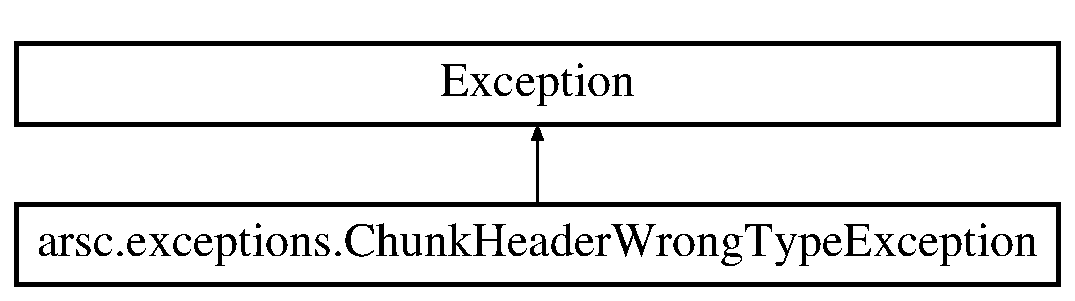
\includegraphics[height=2.000000cm]{classarsc_1_1exceptions_1_1ChunkHeaderWrongTypeException}
\end{center}
\end{figure}
\subsection*{Public Member Functions}
\begin{DoxyCompactItemize}
\item 
\mbox{\Hypertarget{classarsc_1_1exceptions_1_1ChunkHeaderWrongTypeException_abbca025f53d4b228b2ecfe240eebcceb}\label{classarsc_1_1exceptions_1_1ChunkHeaderWrongTypeException_abbca025f53d4b228b2ecfe240eebcceb}} 
def {\bfseries \+\_\+\+\_\+init\+\_\+\+\_\+} (self, expected\+Type, chunk\+Type=None)
\end{DoxyCompactItemize}


The documentation for this class was generated from the following file\+:\begin{DoxyCompactItemize}
\item 
arsc/\mbox{\hyperlink{exceptions_8py}{exceptions.\+py}}\end{DoxyCompactItemize}

\hypertarget{classarsc_1_1config_1_1ResTable__config_1_1Config}{}\section{arsc.\+config.\+Res\+Table\+\_\+config.\+Config Class Reference}
\label{classarsc_1_1config_1_1ResTable__config_1_1Config}\index{arsc.\+config.\+Res\+Table\+\_\+config.\+Config@{arsc.\+config.\+Res\+Table\+\_\+config.\+Config}}
Inheritance diagram for arsc.\+config.\+Res\+Table\+\_\+config.\+Config\+:\begin{figure}[H]
\begin{center}
\leavevmode
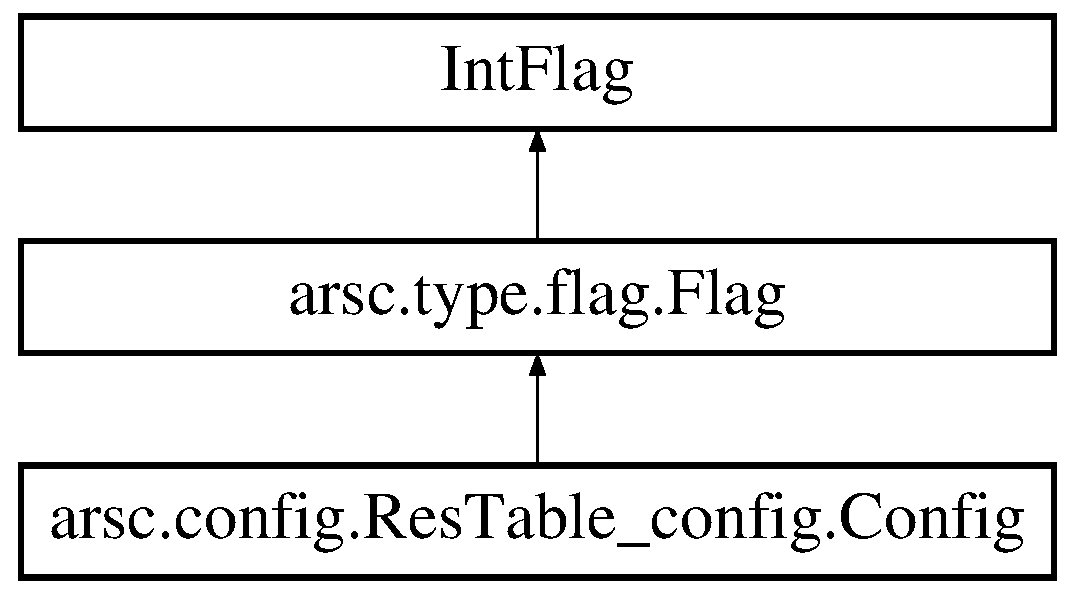
\includegraphics[height=3.000000cm]{classarsc_1_1config_1_1ResTable__config_1_1Config}
\end{center}
\end{figure}
\subsection*{Static Public Attributes}
\begin{DoxyCompactItemize}
\item 
\mbox{\Hypertarget{classarsc_1_1config_1_1ResTable__config_1_1Config_a90841e93421b8925a9e1436a679b0bf5}\label{classarsc_1_1config_1_1ResTable__config_1_1Config_a90841e93421b8925a9e1436a679b0bf5}} 
{\bfseries C\+O\+N\+F\+I\+G\+\_\+\+M\+CC} = A\+Configuration.\+A\+C\+O\+N\+F\+I\+G\+U\+R\+A\+T\+I\+O\+N\+\_\+\+M\+CC
\item 
\mbox{\Hypertarget{classarsc_1_1config_1_1ResTable__config_1_1Config_ad5867551dad1df8984a78b9db0971a80}\label{classarsc_1_1config_1_1ResTable__config_1_1Config_ad5867551dad1df8984a78b9db0971a80}} 
{\bfseries C\+O\+N\+F\+I\+G\+\_\+\+M\+NC} = A\+Configuration.\+A\+C\+O\+N\+F\+I\+G\+U\+R\+A\+T\+I\+O\+N\+\_\+\+M\+CC
\item 
\mbox{\Hypertarget{classarsc_1_1config_1_1ResTable__config_1_1Config_a2adb9febee99f9c36c3f82b9a1939a8e}\label{classarsc_1_1config_1_1ResTable__config_1_1Config_a2adb9febee99f9c36c3f82b9a1939a8e}} 
{\bfseries C\+O\+N\+F\+I\+G\+\_\+\+L\+O\+C\+A\+LE} = A\+Configuration.\+A\+C\+O\+N\+F\+I\+G\+U\+R\+A\+T\+I\+O\+N\+\_\+\+L\+O\+C\+A\+LE
\item 
\mbox{\Hypertarget{classarsc_1_1config_1_1ResTable__config_1_1Config_ad4ccabba6554e7222233feb51b84384c}\label{classarsc_1_1config_1_1ResTable__config_1_1Config_ad4ccabba6554e7222233feb51b84384c}} 
{\bfseries C\+O\+N\+F\+I\+G\+\_\+\+T\+O\+U\+C\+H\+S\+C\+R\+E\+EN} = A\+Configuration.\+A\+C\+O\+N\+F\+I\+G\+U\+R\+A\+T\+I\+O\+N\+\_\+\+T\+O\+U\+C\+H\+S\+C\+R\+E\+EN
\item 
\mbox{\Hypertarget{classarsc_1_1config_1_1ResTable__config_1_1Config_a9f58a30cfba51796a7c7de7b31949df9}\label{classarsc_1_1config_1_1ResTable__config_1_1Config_a9f58a30cfba51796a7c7de7b31949df9}} 
{\bfseries C\+O\+N\+F\+I\+G\+\_\+\+K\+E\+Y\+B\+O\+A\+RD} = A\+Configuration.\+A\+C\+O\+N\+F\+I\+G\+U\+R\+A\+T\+I\+O\+N\+\_\+\+K\+E\+Y\+B\+O\+A\+RD
\item 
\mbox{\Hypertarget{classarsc_1_1config_1_1ResTable__config_1_1Config_aa7da52ea42e31da125ceb8d407ca5f4e}\label{classarsc_1_1config_1_1ResTable__config_1_1Config_aa7da52ea42e31da125ceb8d407ca5f4e}} 
{\bfseries C\+O\+N\+F\+I\+G\+\_\+\+K\+E\+Y\+B\+O\+A\+R\+D\+\_\+\+H\+I\+D\+D\+EN} = A\+Configuration.\+A\+C\+O\+N\+F\+I\+G\+U\+R\+A\+T\+I\+O\+N\+\_\+\+K\+E\+Y\+B\+O\+A\+R\+D\+\_\+\+H\+I\+D\+D\+EN
\item 
\mbox{\Hypertarget{classarsc_1_1config_1_1ResTable__config_1_1Config_aecb1f0472c10d9268cf52bdd842980ae}\label{classarsc_1_1config_1_1ResTable__config_1_1Config_aecb1f0472c10d9268cf52bdd842980ae}} 
{\bfseries C\+O\+N\+F\+I\+G\+\_\+\+N\+A\+V\+I\+G\+A\+T\+I\+ON} = A\+Configuration.\+A\+C\+O\+N\+F\+I\+G\+U\+R\+A\+T\+I\+O\+N\+\_\+\+N\+A\+V\+I\+G\+A\+T\+I\+ON
\item 
\mbox{\Hypertarget{classarsc_1_1config_1_1ResTable__config_1_1Config_a6f445f01c36f766367b753751f4ec00d}\label{classarsc_1_1config_1_1ResTable__config_1_1Config_a6f445f01c36f766367b753751f4ec00d}} 
{\bfseries C\+O\+N\+F\+I\+G\+\_\+\+O\+R\+I\+E\+N\+T\+A\+T\+I\+ON} = A\+Configuration.\+A\+C\+O\+N\+F\+I\+G\+U\+R\+A\+T\+I\+O\+N\+\_\+\+O\+R\+I\+E\+N\+T\+A\+T\+I\+ON
\item 
\mbox{\Hypertarget{classarsc_1_1config_1_1ResTable__config_1_1Config_aff042ce88ac58d29b9fdd4b925e34b8d}\label{classarsc_1_1config_1_1ResTable__config_1_1Config_aff042ce88ac58d29b9fdd4b925e34b8d}} 
{\bfseries C\+O\+N\+F\+I\+G\+\_\+\+D\+E\+N\+S\+I\+TY} = A\+Configuration.\+A\+C\+O\+N\+F\+I\+G\+U\+R\+A\+T\+I\+O\+N\+\_\+\+D\+E\+N\+S\+I\+TY
\item 
\mbox{\Hypertarget{classarsc_1_1config_1_1ResTable__config_1_1Config_a19e3c028738a69f5b365ad6514fa2975}\label{classarsc_1_1config_1_1ResTable__config_1_1Config_a19e3c028738a69f5b365ad6514fa2975}} 
{\bfseries C\+O\+N\+F\+I\+G\+\_\+\+S\+C\+R\+E\+E\+N\+\_\+\+S\+I\+ZE} = A\+Configuration.\+A\+C\+O\+N\+F\+I\+G\+U\+R\+A\+T\+I\+O\+N\+\_\+\+S\+C\+R\+E\+E\+N\+\_\+\+S\+I\+ZE
\item 
\mbox{\Hypertarget{classarsc_1_1config_1_1ResTable__config_1_1Config_a0cb667c5bd2cd0f00dbc72448f58968f}\label{classarsc_1_1config_1_1ResTable__config_1_1Config_a0cb667c5bd2cd0f00dbc72448f58968f}} 
{\bfseries C\+O\+N\+F\+I\+G\+\_\+\+S\+M\+A\+L\+L\+E\+S\+T\+\_\+\+S\+C\+R\+E\+E\+N\+\_\+\+S\+I\+ZE} = A\+Configuration.\+A\+C\+O\+N\+F\+I\+G\+U\+R\+A\+T\+I\+O\+N\+\_\+\+S\+M\+A\+L\+L\+E\+S\+T\+\_\+\+S\+C\+R\+E\+E\+N\+\_\+\+S\+I\+ZE
\item 
\mbox{\Hypertarget{classarsc_1_1config_1_1ResTable__config_1_1Config_ad5afe77e59294d4362738963c456cbe8}\label{classarsc_1_1config_1_1ResTable__config_1_1Config_ad5afe77e59294d4362738963c456cbe8}} 
{\bfseries C\+O\+N\+F\+I\+G\+\_\+\+V\+E\+R\+S\+I\+ON} = A\+Configuration.\+A\+C\+O\+N\+F\+I\+G\+U\+R\+A\+T\+I\+O\+N\+\_\+\+V\+E\+R\+S\+I\+ON
\item 
\mbox{\Hypertarget{classarsc_1_1config_1_1ResTable__config_1_1Config_a4ee41f82ff964ce64bcdb49c23eb715e}\label{classarsc_1_1config_1_1ResTable__config_1_1Config_a4ee41f82ff964ce64bcdb49c23eb715e}} 
{\bfseries C\+O\+N\+F\+I\+G\+\_\+\+S\+C\+R\+E\+E\+N\+\_\+\+L\+A\+Y\+O\+UT} = A\+Configuration.\+A\+C\+O\+N\+F\+I\+G\+U\+R\+A\+T\+I\+O\+N\+\_\+\+S\+C\+R\+E\+E\+N\+\_\+\+L\+A\+Y\+O\+UT
\item 
\mbox{\Hypertarget{classarsc_1_1config_1_1ResTable__config_1_1Config_a49d212b1575ba404d072b46a691c17b9}\label{classarsc_1_1config_1_1ResTable__config_1_1Config_a49d212b1575ba404d072b46a691c17b9}} 
{\bfseries C\+O\+N\+F\+I\+G\+\_\+\+U\+I\+\_\+\+M\+O\+DE} = A\+Configuration.\+A\+C\+O\+N\+F\+I\+G\+U\+R\+A\+T\+I\+O\+N\+\_\+\+U\+I\+\_\+\+M\+O\+DE
\item 
\mbox{\Hypertarget{classarsc_1_1config_1_1ResTable__config_1_1Config_a4dcae56207d064f1d2ea3f67f542bae0}\label{classarsc_1_1config_1_1ResTable__config_1_1Config_a4dcae56207d064f1d2ea3f67f542bae0}} 
{\bfseries C\+O\+N\+F\+I\+G\+\_\+\+L\+A\+Y\+O\+U\+T\+D\+IR} = A\+Configuration.\+A\+C\+O\+N\+F\+I\+G\+U\+R\+A\+T\+I\+O\+N\+\_\+\+L\+A\+Y\+O\+U\+T\+D\+IR
\item 
\mbox{\Hypertarget{classarsc_1_1config_1_1ResTable__config_1_1Config_a3d8b3f66fa630698badcd40397f61549}\label{classarsc_1_1config_1_1ResTable__config_1_1Config_a3d8b3f66fa630698badcd40397f61549}} 
int {\bfseries C\+O\+N\+F\+I\+G\+\_\+\+M\+AX} = 0xffffffff
\end{DoxyCompactItemize}
\subsection*{Additional Inherited Members}


The documentation for this class was generated from the following file\+:\begin{DoxyCompactItemize}
\item 
arsc/\mbox{\hyperlink{config_8py}{config.\+py}}\end{DoxyCompactItemize}

\hypertarget{classarsc_1_1type_1_1enum_1_1Enum}{}\section{arsc.\+type.\+enum.\+Enum Class Reference}
\label{classarsc_1_1type_1_1enum_1_1Enum}\index{arsc.\+type.\+enum.\+Enum@{arsc.\+type.\+enum.\+Enum}}
Inheritance diagram for arsc.\+type.\+enum.\+Enum\+:\begin{figure}[H]
\begin{center}
\leavevmode
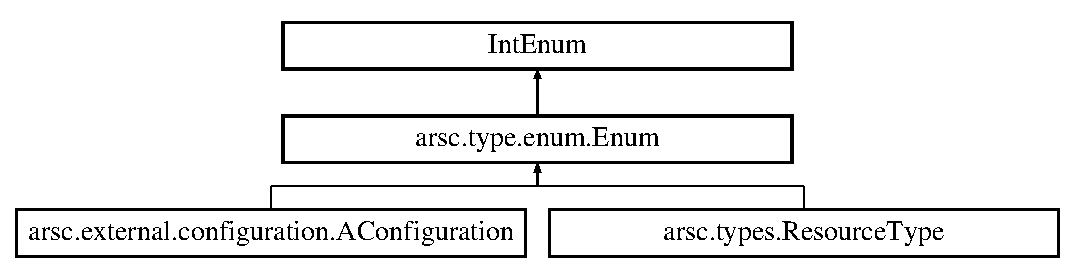
\includegraphics[height=3.000000cm]{classarsc_1_1type_1_1enum_1_1Enum}
\end{center}
\end{figure}
\subsection*{Public Member Functions}
\begin{DoxyCompactItemize}
\item 
\mbox{\Hypertarget{classarsc_1_1type_1_1enum_1_1Enum_a58f05278b7419febc1b4344ca3ec1ef0}\label{classarsc_1_1type_1_1enum_1_1Enum_a58f05278b7419febc1b4344ca3ec1ef0}} 
def {\bfseries \+\_\+\+\_\+bytes\+\_\+\+\_\+} (self)
\item 
\mbox{\Hypertarget{classarsc_1_1type_1_1enum_1_1Enum_affa0c921e9b1b2f4b754bd8362d1d106}\label{classarsc_1_1type_1_1enum_1_1Enum_affa0c921e9b1b2f4b754bd8362d1d106}} 
def {\bfseries \+\_\+\+\_\+len\+\_\+\+\_\+} (self)
\item 
\mbox{\Hypertarget{classarsc_1_1type_1_1enum_1_1Enum_ac86ef29fae31eb07e6e62ee554f5e8f2}\label{classarsc_1_1type_1_1enum_1_1Enum_ac86ef29fae31eb07e6e62ee554f5e8f2}} 
def {\bfseries from\+\_\+bytes} (cls, b, little=False)
\end{DoxyCompactItemize}


The documentation for this class was generated from the following file\+:\begin{DoxyCompactItemize}
\item 
arsc/type/\mbox{\hyperlink{enum_8py}{enum.\+py}}\end{DoxyCompactItemize}

\hypertarget{classarsc_1_1type_1_1flag_1_1Flag}{}\section{arsc.\+type.\+flag.\+Flag Class Reference}
\label{classarsc_1_1type_1_1flag_1_1Flag}\index{arsc.\+type.\+flag.\+Flag@{arsc.\+type.\+flag.\+Flag}}
Inheritance diagram for arsc.\+type.\+flag.\+Flag\+:\begin{figure}[H]
\begin{center}
\leavevmode
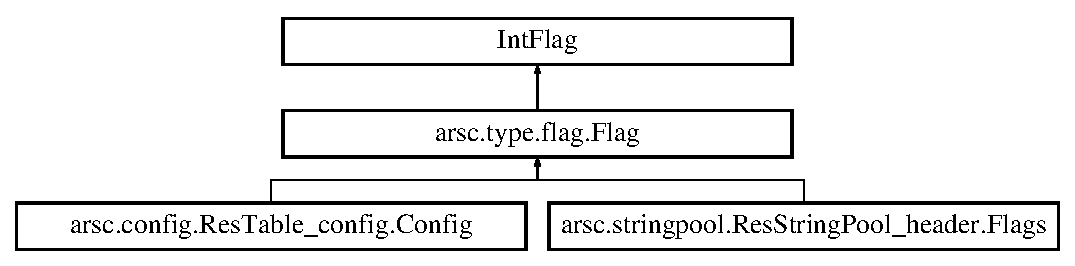
\includegraphics[height=3.000000cm]{classarsc_1_1type_1_1flag_1_1Flag}
\end{center}
\end{figure}
\subsection*{Public Member Functions}
\begin{DoxyCompactItemize}
\item 
\mbox{\Hypertarget{classarsc_1_1type_1_1flag_1_1Flag_a3b55dd3f42de1c244551d80b72776036}\label{classarsc_1_1type_1_1flag_1_1Flag_a3b55dd3f42de1c244551d80b72776036}} 
def {\bfseries \+\_\+\+\_\+bytes\+\_\+\+\_\+} (self)
\item 
\mbox{\Hypertarget{classarsc_1_1type_1_1flag_1_1Flag_a7d2f6513250191ea8042d6d07deed23e}\label{classarsc_1_1type_1_1flag_1_1Flag_a7d2f6513250191ea8042d6d07deed23e}} 
def {\bfseries \+\_\+\+\_\+len\+\_\+\+\_\+} (self)
\item 
\mbox{\Hypertarget{classarsc_1_1type_1_1flag_1_1Flag_aadc826a24e4ca3e1b905d81d02865da9}\label{classarsc_1_1type_1_1flag_1_1Flag_aadc826a24e4ca3e1b905d81d02865da9}} 
def {\bfseries from\+\_\+bytes} (cls, b, little=False)
\end{DoxyCompactItemize}


The documentation for this class was generated from the following file\+:\begin{DoxyCompactItemize}
\item 
arsc/type/\mbox{\hyperlink{flag_8py}{flag.\+py}}\end{DoxyCompactItemize}

\hypertarget{classarsc_1_1stringpool_1_1ResStringPool__header_1_1Flags}{}\section{arsc.\+stringpool.\+Res\+String\+Pool\+\_\+header.\+Flags Class Reference}
\label{classarsc_1_1stringpool_1_1ResStringPool__header_1_1Flags}\index{arsc.\+stringpool.\+Res\+String\+Pool\+\_\+header.\+Flags@{arsc.\+stringpool.\+Res\+String\+Pool\+\_\+header.\+Flags}}
Inheritance diagram for arsc.\+stringpool.\+Res\+String\+Pool\+\_\+header.\+Flags\+:\begin{figure}[H]
\begin{center}
\leavevmode
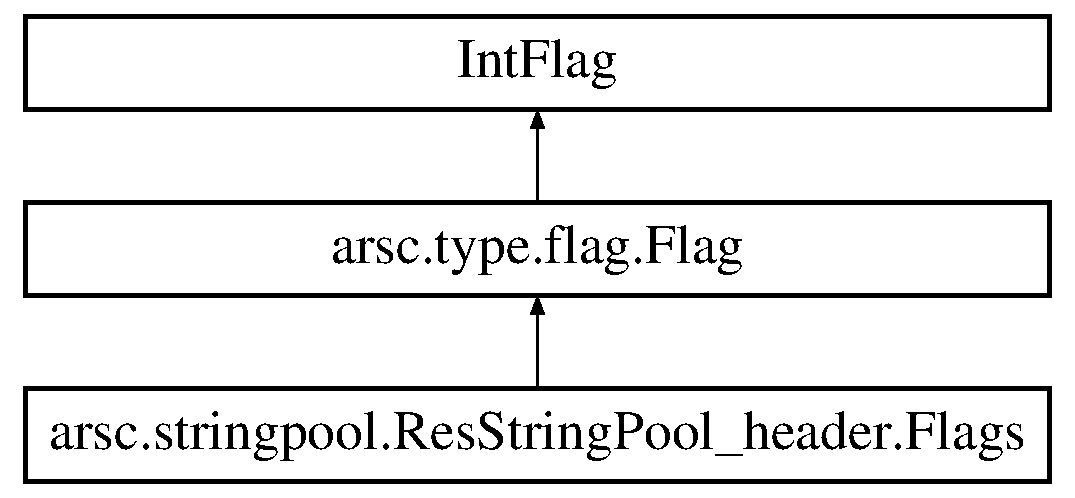
\includegraphics[height=3.000000cm]{classarsc_1_1stringpool_1_1ResStringPool__header_1_1Flags}
\end{center}
\end{figure}
\subsection*{Static Public Attributes}
\begin{DoxyCompactItemize}
\item 
int \mbox{\hyperlink{classarsc_1_1stringpool_1_1ResStringPool__header_1_1Flags_af354a9864bce5baf864b5c5ea951bead}{S\+O\+R\+T\+E\+D\+\_\+\+F\+L\+AG}} = 0x1
\begin{DoxyCompactList}\small\item\em If set, the string index is sorted by the string values (based on strcmp16()). \end{DoxyCompactList}\item 
\mbox{\Hypertarget{classarsc_1_1stringpool_1_1ResStringPool__header_1_1Flags_a58e87ceaf5312e23a80606d2584c7c52}\label{classarsc_1_1stringpool_1_1ResStringPool__header_1_1Flags_a58e87ceaf5312e23a80606d2584c7c52}} 
int \mbox{\hyperlink{classarsc_1_1stringpool_1_1ResStringPool__header_1_1Flags_a58e87ceaf5312e23a80606d2584c7c52}{U\+T\+F8\+\_\+\+F\+L\+AG}} = 0x100
\begin{DoxyCompactList}\small\item\em String pool is encoded in U\+T\+F-\/8. \end{DoxyCompactList}\item 
\mbox{\Hypertarget{classarsc_1_1stringpool_1_1ResStringPool__header_1_1Flags_afe8f5b6207d6732e9430600b0922c47e}\label{classarsc_1_1stringpool_1_1ResStringPool__header_1_1Flags_afe8f5b6207d6732e9430600b0922c47e}} 
int {\bfseries M\+AX} = 0xffffffff
\end{DoxyCompactItemize}
\subsection*{Additional Inherited Members}


\subsection{Member Data Documentation}
\mbox{\Hypertarget{classarsc_1_1stringpool_1_1ResStringPool__header_1_1Flags_af354a9864bce5baf864b5c5ea951bead}\label{classarsc_1_1stringpool_1_1ResStringPool__header_1_1Flags_af354a9864bce5baf864b5c5ea951bead}} 
\index{arsc\+::stringpool\+::\+Res\+String\+Pool\+\_\+header\+::\+Flags@{arsc\+::stringpool\+::\+Res\+String\+Pool\+\_\+header\+::\+Flags}!S\+O\+R\+T\+E\+D\+\_\+\+F\+L\+AG@{S\+O\+R\+T\+E\+D\+\_\+\+F\+L\+AG}}
\index{S\+O\+R\+T\+E\+D\+\_\+\+F\+L\+AG@{S\+O\+R\+T\+E\+D\+\_\+\+F\+L\+AG}!arsc\+::stringpool\+::\+Res\+String\+Pool\+\_\+header\+::\+Flags@{arsc\+::stringpool\+::\+Res\+String\+Pool\+\_\+header\+::\+Flags}}
\subsubsection{\texorpdfstring{S\+O\+R\+T\+E\+D\+\_\+\+F\+L\+AG}{SORTED\_FLAG}}
{\footnotesize\ttfamily int arsc.\+stringpool.\+Res\+String\+Pool\+\_\+header.\+Flags.\+S\+O\+R\+T\+E\+D\+\_\+\+F\+L\+AG = 0x1\hspace{0.3cm}{\ttfamily [static]}}



If set, the string index is sorted by the string values (based on strcmp16()). 



The documentation for this class was generated from the following file\+:\begin{DoxyCompactItemize}
\item 
arsc/\mbox{\hyperlink{stringpool_8py}{stringpool.\+py}}\end{DoxyCompactItemize}

\hypertarget{classarsc_1_1config_1_1ResTable__config_1_1Imsi}{}\section{arsc.\+config.\+Res\+Table\+\_\+config.\+Imsi Class Reference}
\label{classarsc_1_1config_1_1ResTable__config_1_1Imsi}\index{arsc.\+config.\+Res\+Table\+\_\+config.\+Imsi@{arsc.\+config.\+Res\+Table\+\_\+config.\+Imsi}}


Filter based on M\+CC and M\+NC.  


\subsection*{Public Member Functions}
\begin{DoxyCompactItemize}
\item 
\mbox{\Hypertarget{classarsc_1_1config_1_1ResTable__config_1_1Imsi_a43f78480e529c7a032be43e18344b626}\label{classarsc_1_1config_1_1ResTable__config_1_1Imsi_a43f78480e529c7a032be43e18344b626}} 
def {\bfseries \+\_\+\+\_\+init\+\_\+\+\_\+} (self, \mbox{\hyperlink{classarsc_1_1config_1_1ResTable__config_1_1Imsi_aab990d0a363a63813c0d686ae7e1f54b}{mcc}}=0, \mbox{\hyperlink{classarsc_1_1config_1_1ResTable__config_1_1Imsi_acf991b66dce86e39c571064fa23f08ad}{mnc}}=0)
\end{DoxyCompactItemize}
\subsection*{Public Attributes}
\begin{DoxyCompactItemize}
\item 
\mbox{\Hypertarget{classarsc_1_1config_1_1ResTable__config_1_1Imsi_aab990d0a363a63813c0d686ae7e1f54b}\label{classarsc_1_1config_1_1ResTable__config_1_1Imsi_aab990d0a363a63813c0d686ae7e1f54b}} 
\mbox{\hyperlink{classarsc_1_1config_1_1ResTable__config_1_1Imsi_aab990d0a363a63813c0d686ae7e1f54b}{mcc}}
\begin{DoxyCompactList}\small\item\em Mobile Country Code. \end{DoxyCompactList}\item 
\mbox{\Hypertarget{classarsc_1_1config_1_1ResTable__config_1_1Imsi_acf991b66dce86e39c571064fa23f08ad}\label{classarsc_1_1config_1_1ResTable__config_1_1Imsi_acf991b66dce86e39c571064fa23f08ad}} 
\mbox{\hyperlink{classarsc_1_1config_1_1ResTable__config_1_1Imsi_acf991b66dce86e39c571064fa23f08ad}{mnc}}
\begin{DoxyCompactList}\small\item\em Mobile Network Code. \end{DoxyCompactList}\end{DoxyCompactItemize}


\subsection{Detailed Description}
Filter based on M\+CC and M\+NC. 

The documentation for this class was generated from the following file\+:\begin{DoxyCompactItemize}
\item 
arsc/\mbox{\hyperlink{config_8py}{config.\+py}}\end{DoxyCompactItemize}

\hypertarget{classarsc_1_1config_1_1ResTable__config_1_1Input}{}\section{arsc.\+config.\+Res\+Table\+\_\+config.\+Input Class Reference}
\label{classarsc_1_1config_1_1ResTable__config_1_1Input}\index{arsc.\+config.\+Res\+Table\+\_\+config.\+Input@{arsc.\+config.\+Res\+Table\+\_\+config.\+Input}}


The documentation for this class was generated from the following file\+:\begin{DoxyCompactItemize}
\item 
arsc/\mbox{\hyperlink{config_8py}{config.\+py}}\end{DoxyCompactItemize}

\hypertarget{classarsc_1_1config_1_1ResTable__config_1_1Locale}{}\section{arsc.\+config.\+Res\+Table\+\_\+config.\+Locale Class Reference}
\label{classarsc_1_1config_1_1ResTable__config_1_1Locale}\index{arsc.\+config.\+Res\+Table\+\_\+config.\+Locale@{arsc.\+config.\+Res\+Table\+\_\+config.\+Locale}}


Filter based on language and country.  


\subsection*{Public Member Functions}
\begin{DoxyCompactItemize}
\item 
\mbox{\Hypertarget{classarsc_1_1config_1_1ResTable__config_1_1Locale_acdb0865b2fd5e8d9a957e1e8dbc946b8}\label{classarsc_1_1config_1_1ResTable__config_1_1Locale_acdb0865b2fd5e8d9a957e1e8dbc946b8}} 
def {\bfseries \+\_\+\+\_\+init\+\_\+\+\_\+} (self, language=b\textquotesingle{}\textbackslash{}0\textbackslash{}0\textquotesingle{}, country=b\textquotesingle{}\textbackslash{}0\textbackslash{}0\textquotesingle{})
\end{DoxyCompactItemize}


\subsection{Detailed Description}
Filter based on language and country. 

The documentation for this class was generated from the following file\+:\begin{DoxyCompactItemize}
\item 
arsc/\mbox{\hyperlink{config_8py}{config.\+py}}\end{DoxyCompactItemize}

\hypertarget{classarsc_1_1chunk_1_1ResChunk__header}{}\section{arsc.\+chunk.\+Res\+Chunk\+\_\+header Class Reference}
\label{classarsc_1_1chunk_1_1ResChunk__header}\index{arsc.\+chunk.\+Res\+Chunk\+\_\+header@{arsc.\+chunk.\+Res\+Chunk\+\_\+header}}


Header that appears at the front of every data chunk in a resource.  


\subsection*{Public Member Functions}
\begin{DoxyCompactItemize}
\item 
\mbox{\Hypertarget{classarsc_1_1chunk_1_1ResChunk__header_a2058bbcf356ca56b29153ff9a065abc6}\label{classarsc_1_1chunk_1_1ResChunk__header_a2058bbcf356ca56b29153ff9a065abc6}} 
def {\bfseries \+\_\+\+\_\+init\+\_\+\+\_\+} (self, chunk\+Type=Resource\+Type.\+R\+E\+S\+\_\+\+N\+U\+L\+L\+\_\+\+T\+Y\+PE, header\+Size=Res\+Chunk\+\_\+header\+\_\+len, size=Res\+Chunk\+\_\+header\+\_\+len)
\item 
\mbox{\Hypertarget{classarsc_1_1chunk_1_1ResChunk__header_a34d6403d6edce7fb369b3d6933c27dee}\label{classarsc_1_1chunk_1_1ResChunk__header_a34d6403d6edce7fb369b3d6933c27dee}} 
def {\bfseries \+\_\+\+\_\+str\+\_\+\+\_\+} (self)
\item 
\mbox{\Hypertarget{classarsc_1_1chunk_1_1ResChunk__header_a7a5f16c8263a193898e7ed2619a4082c}\label{classarsc_1_1chunk_1_1ResChunk__header_a7a5f16c8263a193898e7ed2619a4082c}} 
def {\bfseries \+\_\+\+\_\+repr\+\_\+\+\_\+} (self)
\item 
\mbox{\Hypertarget{classarsc_1_1chunk_1_1ResChunk__header_ab148b08c983975777f31ed8bb958b74e}\label{classarsc_1_1chunk_1_1ResChunk__header_ab148b08c983975777f31ed8bb958b74e}} 
def {\bfseries \+\_\+\+\_\+eq\+\_\+\+\_\+} (self, rhs)
\item 
\mbox{\Hypertarget{classarsc_1_1chunk_1_1ResChunk__header_a3a0104e929b75484360f38bcf68cff38}\label{classarsc_1_1chunk_1_1ResChunk__header_a3a0104e929b75484360f38bcf68cff38}} 
def {\bfseries \+\_\+\+\_\+len\+\_\+\+\_\+} (self)
\item 
\mbox{\Hypertarget{classarsc_1_1chunk_1_1ResChunk__header_ab8196245262c3ef25430ee683ea1f26d}\label{classarsc_1_1chunk_1_1ResChunk__header_ab8196245262c3ef25430ee683ea1f26d}} 
def {\bfseries \+\_\+\+\_\+bytes\+\_\+\+\_\+} (self)
\item 
\mbox{\Hypertarget{classarsc_1_1chunk_1_1ResChunk__header_abd99a20cd5e78716a2655867787c0672}\label{classarsc_1_1chunk_1_1ResChunk__header_abd99a20cd5e78716a2655867787c0672}} 
def {\bfseries from\+\_\+bytes} (b, little=True)
\end{DoxyCompactItemize}
\subsection*{Public Attributes}
\begin{DoxyCompactItemize}
\item 
\mbox{\Hypertarget{classarsc_1_1chunk_1_1ResChunk__header_a0521ef18ea2ec7881730f849a97a5e82}\label{classarsc_1_1chunk_1_1ResChunk__header_a0521ef18ea2ec7881730f849a97a5e82}} 
{\bfseries type}
\item 
\mbox{\Hypertarget{classarsc_1_1chunk_1_1ResChunk__header_ae735969556a68c5cc1d397a20794b528}\label{classarsc_1_1chunk_1_1ResChunk__header_ae735969556a68c5cc1d397a20794b528}} 
{\bfseries header\+Size}
\item 
\mbox{\Hypertarget{classarsc_1_1chunk_1_1ResChunk__header_acf998f9b9197f0596f90778335ab8c68}\label{classarsc_1_1chunk_1_1ResChunk__header_acf998f9b9197f0596f90778335ab8c68}} 
{\bfseries size}
\end{DoxyCompactItemize}
\subsection*{Static Public Attributes}
\begin{DoxyCompactItemize}
\item 
\mbox{\Hypertarget{classarsc_1_1chunk_1_1ResChunk__header_a20130351bf48d2789d4abc2939c8052f}\label{classarsc_1_1chunk_1_1ResChunk__header_a20130351bf48d2789d4abc2939c8052f}} 
{\bfseries Res\+Chunk\+\_\+header\+\_\+len} = len(Resource\+Type.\+R\+E\+S\+\_\+\+N\+U\+L\+L\+\_\+\+T\+Y\+PE) + len(\mbox{\hyperlink{classarsc_1_1type_1_1uint16_1_1uint16}{uint16}}(0)) + \textbackslash{}
\end{DoxyCompactItemize}


\subsection{Detailed Description}
Header that appears at the front of every data chunk in a resource. 



The documentation for this class was generated from the following file\+:\begin{DoxyCompactItemize}
\item 
arsc/\mbox{\hyperlink{chunk_8py}{chunk.\+py}}\end{DoxyCompactItemize}

\hypertarget{classarsc_1_1types_1_1ResourceType}{}\section{arsc.\+types.\+Resource\+Type Class Reference}
\label{classarsc_1_1types_1_1ResourceType}\index{arsc.\+types.\+Resource\+Type@{arsc.\+types.\+Resource\+Type}}
Inheritance diagram for arsc.\+types.\+Resource\+Type\+:\begin{figure}[H]
\begin{center}
\leavevmode
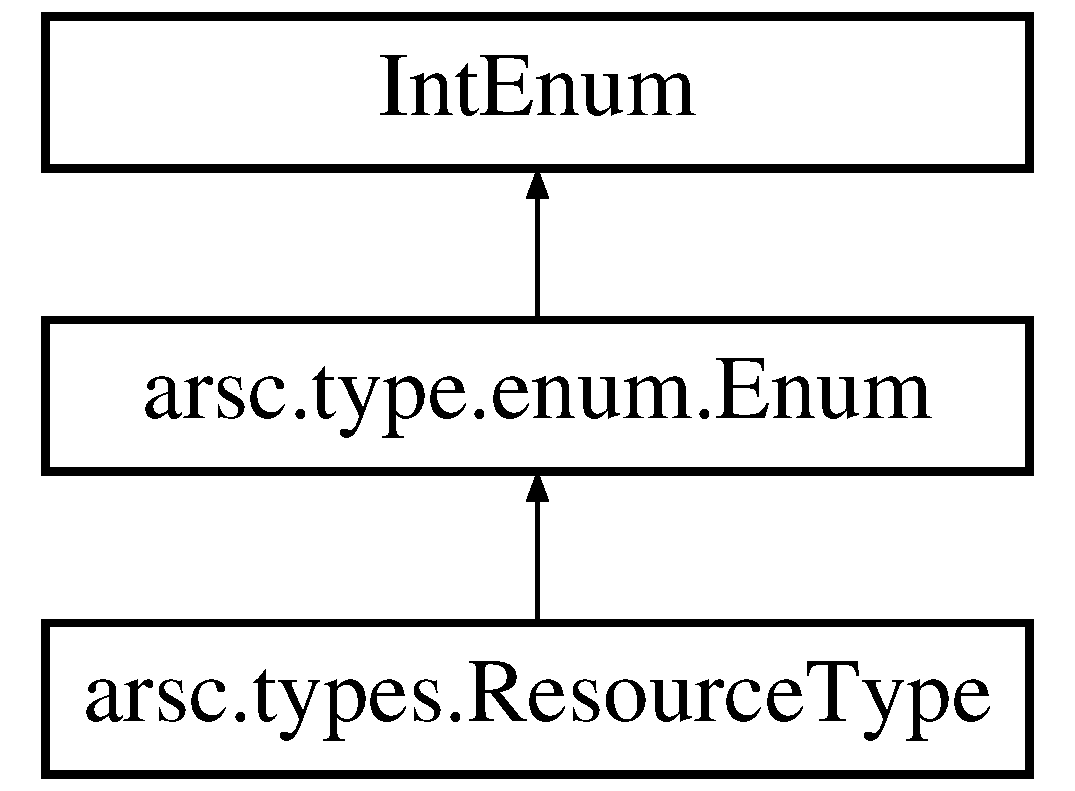
\includegraphics[height=3.000000cm]{classarsc_1_1types_1_1ResourceType}
\end{center}
\end{figure}
\subsection*{Static Public Attributes}
\begin{DoxyCompactItemize}
\item 
\mbox{\Hypertarget{classarsc_1_1types_1_1ResourceType_af1786a9013371730067939e2eb77e530}\label{classarsc_1_1types_1_1ResourceType_af1786a9013371730067939e2eb77e530}} 
int {\bfseries R\+E\+S\+\_\+\+N\+U\+L\+L\+\_\+\+T\+Y\+PE} = 0x0000
\item 
\mbox{\Hypertarget{classarsc_1_1types_1_1ResourceType_afb1b1cbec751d3ba92ee0cb722f8987c}\label{classarsc_1_1types_1_1ResourceType_afb1b1cbec751d3ba92ee0cb722f8987c}} 
int \mbox{\hyperlink{classarsc_1_1types_1_1ResourceType_afb1b1cbec751d3ba92ee0cb722f8987c}{R\+E\+S\+\_\+\+S\+T\+R\+I\+N\+G\+\_\+\+P\+O\+O\+L\+\_\+\+T\+Y\+PE}} = 0x0001
\begin{DoxyCompactList}\small\item\em Res\+Chunk\+\_\+header is part of \mbox{\hyperlink{classarsc_1_1stringpool_1_1ResStringPool}{stringpool.\+Res\+String\+Pool}}. \end{DoxyCompactList}\item 
\mbox{\Hypertarget{classarsc_1_1types_1_1ResourceType_aa09309a3e24293829bf8856338eb839a}\label{classarsc_1_1types_1_1ResourceType_aa09309a3e24293829bf8856338eb839a}} 
int \mbox{\hyperlink{classarsc_1_1types_1_1ResourceType_aa09309a3e24293829bf8856338eb839a}{R\+E\+S\+\_\+\+T\+A\+B\+L\+E\+\_\+\+T\+Y\+PE}} = 0x0002
\begin{DoxyCompactList}\small\item\em Res\+Chunk\+\_\+header is part of \mbox{\hyperlink{classarsc_1_1table_1_1ResTable__header}{table.\+Res\+Table\+\_\+header}}. \end{DoxyCompactList}\item 
\mbox{\Hypertarget{classarsc_1_1types_1_1ResourceType_ae53161d035e110d9dd276b64e64dc008}\label{classarsc_1_1types_1_1ResourceType_ae53161d035e110d9dd276b64e64dc008}} 
int {\bfseries R\+E\+S\+\_\+\+X\+M\+L\+\_\+\+T\+Y\+PE} = 0x0003
\item 
\mbox{\Hypertarget{classarsc_1_1types_1_1ResourceType_a51d4489b5023ea85c6233c74730afc82}\label{classarsc_1_1types_1_1ResourceType_a51d4489b5023ea85c6233c74730afc82}} 
int {\bfseries R\+E\+S\+\_\+\+X\+M\+L\+\_\+\+F\+I\+R\+S\+T\+\_\+\+C\+H\+U\+N\+K\+\_\+\+T\+Y\+PE} = 0x0100
\item 
\mbox{\Hypertarget{classarsc_1_1types_1_1ResourceType_a9043b7e6fcf74bd7369036bbe04a7be1}\label{classarsc_1_1types_1_1ResourceType_a9043b7e6fcf74bd7369036bbe04a7be1}} 
int {\bfseries R\+E\+S\+\_\+\+X\+M\+L\+\_\+\+S\+T\+A\+R\+T\+\_\+\+N\+A\+M\+E\+S\+P\+A\+C\+E\+\_\+\+T\+Y\+PE} = 0x0100
\item 
\mbox{\Hypertarget{classarsc_1_1types_1_1ResourceType_a2a9cbb196e182bf913c04758cac9e0ed}\label{classarsc_1_1types_1_1ResourceType_a2a9cbb196e182bf913c04758cac9e0ed}} 
int {\bfseries R\+E\+S\+\_\+\+X\+M\+L\+\_\+\+E\+N\+D\+\_\+\+N\+A\+M\+E\+S\+P\+A\+C\+E\+\_\+\+T\+Y\+PE} = 0x0101
\item 
\mbox{\Hypertarget{classarsc_1_1types_1_1ResourceType_ad3eb3f46404de1ac0f632a3e3a901df3}\label{classarsc_1_1types_1_1ResourceType_ad3eb3f46404de1ac0f632a3e3a901df3}} 
int {\bfseries R\+E\+S\+\_\+\+X\+M\+L\+\_\+\+S\+T\+A\+R\+T\+\_\+\+E\+L\+E\+M\+E\+N\+T\+\_\+\+T\+Y\+PE} = 0x0102
\item 
\mbox{\Hypertarget{classarsc_1_1types_1_1ResourceType_a82d25885a2d13b186763931fb30846a0}\label{classarsc_1_1types_1_1ResourceType_a82d25885a2d13b186763931fb30846a0}} 
int {\bfseries R\+E\+S\+\_\+\+X\+M\+L\+\_\+\+E\+N\+D\+\_\+\+E\+L\+E\+M\+E\+N\+T\+\_\+\+T\+Y\+PE} = 0x0103
\item 
\mbox{\Hypertarget{classarsc_1_1types_1_1ResourceType_ae4c63892ff4be212922ad684c0025481}\label{classarsc_1_1types_1_1ResourceType_ae4c63892ff4be212922ad684c0025481}} 
int {\bfseries R\+E\+S\+\_\+\+X\+M\+L\+\_\+\+C\+D\+A\+T\+A\+\_\+\+T\+Y\+PE} = 0x0104
\item 
\mbox{\Hypertarget{classarsc_1_1types_1_1ResourceType_a061827387bff8ae6bb638f8a924019b8}\label{classarsc_1_1types_1_1ResourceType_a061827387bff8ae6bb638f8a924019b8}} 
int {\bfseries R\+E\+S\+\_\+\+X\+M\+L\+\_\+\+L\+A\+S\+T\+\_\+\+C\+H\+U\+N\+K\+\_\+\+T\+Y\+PE} = 0x017f
\item 
\mbox{\Hypertarget{classarsc_1_1types_1_1ResourceType_a7cc8625b2cfa04a8bf8b84202f48b9c6}\label{classarsc_1_1types_1_1ResourceType_a7cc8625b2cfa04a8bf8b84202f48b9c6}} 
int {\bfseries R\+E\+S\+\_\+\+X\+M\+L\+\_\+\+R\+E\+S\+O\+U\+R\+C\+E\+\_\+\+M\+A\+P\+\_\+\+T\+Y\+PE} = 0x0180
\item 
\mbox{\Hypertarget{classarsc_1_1types_1_1ResourceType_a7f0f847a140ef051b215febe579a0165}\label{classarsc_1_1types_1_1ResourceType_a7f0f847a140ef051b215febe579a0165}} 
int \mbox{\hyperlink{classarsc_1_1types_1_1ResourceType_a7f0f847a140ef051b215febe579a0165}{R\+E\+S\+\_\+\+T\+A\+B\+L\+E\+\_\+\+P\+A\+C\+K\+A\+G\+E\+\_\+\+T\+Y\+PE}} = 0x0200
\begin{DoxyCompactList}\small\item\em Res\+Chunk\+\_\+header is part of \mbox{\hyperlink{}{table.\+Res\+Table\+\_\+package}}. \end{DoxyCompactList}\item 
\mbox{\Hypertarget{classarsc_1_1types_1_1ResourceType_ab31998b94a6b145433a8f3836ef7a118}\label{classarsc_1_1types_1_1ResourceType_ab31998b94a6b145433a8f3836ef7a118}} 
int {\bfseries R\+E\+S\+\_\+\+T\+A\+B\+L\+E\+\_\+\+T\+Y\+P\+E\+\_\+\+T\+Y\+PE} = 0x0201
\item 
\mbox{\Hypertarget{classarsc_1_1types_1_1ResourceType_ad482bca4a4ce39083b2b55b3635b351f}\label{classarsc_1_1types_1_1ResourceType_ad482bca4a4ce39083b2b55b3635b351f}} 
int {\bfseries R\+E\+S\+\_\+\+T\+A\+B\+L\+E\+\_\+\+T\+Y\+P\+E\+\_\+\+S\+P\+E\+C\+\_\+\+T\+Y\+PE} = 0x0202
\end{DoxyCompactItemize}
\subsection*{Additional Inherited Members}


The documentation for this class was generated from the following file\+:\begin{DoxyCompactItemize}
\item 
arsc/\mbox{\hyperlink{types_8py}{types.\+py}}\end{DoxyCompactItemize}

\hypertarget{classarsc_1_1stringpool_1_1ResStringPool}{}\section{arsc.\+stringpool.\+Res\+String\+Pool Class Reference}
\label{classarsc_1_1stringpool_1_1ResStringPool}\index{arsc.\+stringpool.\+Res\+String\+Pool@{arsc.\+stringpool.\+Res\+String\+Pool}}
\subsection*{Public Member Functions}
\begin{DoxyCompactItemize}
\item 
\mbox{\Hypertarget{classarsc_1_1stringpool_1_1ResStringPool_adf8610e1abbb658616bc024fd77c7bf8}\label{classarsc_1_1stringpool_1_1ResStringPool_adf8610e1abbb658616bc024fd77c7bf8}} 
def {\bfseries \+\_\+\+\_\+init\+\_\+\+\_\+} (self, \mbox{\hyperlink{classarsc_1_1stringpool_1_1ResStringPool_a8df057b196c2fbaf9a3a4eeeb3ff3357}{header}}=None, \mbox{\hyperlink{classarsc_1_1stringpool_1_1ResStringPool_a3188382e081e43e85d549297ec499ac2}{strrefs}}=None, \mbox{\hyperlink{classarsc_1_1stringpool_1_1ResStringPool_a7264bcbbfd5862a58240c29e9f4655a1}{stylerefs}}=None, \mbox{\hyperlink{classarsc_1_1stringpool_1_1ResStringPool_a04ef90c01b1a31b1e32936e431a2166d}{strings}}=None, \mbox{\hyperlink{classarsc_1_1stringpool_1_1ResStringPool_aa7ac2665b21f6bdd96bf4ed85f7d58ba}{styles}}=None)
\item 
\mbox{\Hypertarget{classarsc_1_1stringpool_1_1ResStringPool_aded4ae4acdb27fc05fb11112b1406ab7}\label{classarsc_1_1stringpool_1_1ResStringPool_aded4ae4acdb27fc05fb11112b1406ab7}} 
def {\bfseries \+\_\+\+\_\+str\+\_\+\+\_\+} (self)
\item 
\mbox{\Hypertarget{classarsc_1_1stringpool_1_1ResStringPool_a38713da2e81a1bf00b5d960f2cee6ce4}\label{classarsc_1_1stringpool_1_1ResStringPool_a38713da2e81a1bf00b5d960f2cee6ce4}} 
def {\bfseries \+\_\+\+\_\+repr\+\_\+\+\_\+} (self)
\item 
\mbox{\Hypertarget{classarsc_1_1stringpool_1_1ResStringPool_a9138a62791b2f6c86898b0d9e2e8cb96}\label{classarsc_1_1stringpool_1_1ResStringPool_a9138a62791b2f6c86898b0d9e2e8cb96}} 
def {\bfseries \+\_\+\+\_\+eq\+\_\+\+\_\+} (self, rhs)
\item 
\mbox{\Hypertarget{classarsc_1_1stringpool_1_1ResStringPool_a9c1372cf1e1a0978b649c3edd0203417}\label{classarsc_1_1stringpool_1_1ResStringPool_a9c1372cf1e1a0978b649c3edd0203417}} 
def {\bfseries \+\_\+\+\_\+len\+\_\+\+\_\+} (self)
\item 
\mbox{\Hypertarget{classarsc_1_1stringpool_1_1ResStringPool_ae81de86d622c9a80ddbddbc94e6cf14d}\label{classarsc_1_1stringpool_1_1ResStringPool_ae81de86d622c9a80ddbddbc94e6cf14d}} 
def {\bfseries \+\_\+\+\_\+bytes\+\_\+\+\_\+} (self)
\item 
\mbox{\Hypertarget{classarsc_1_1stringpool_1_1ResStringPool_ac9aef78bfa1159f62a1debb84911411f}\label{classarsc_1_1stringpool_1_1ResStringPool_ac9aef78bfa1159f62a1debb84911411f}} 
def {\bfseries from\+\_\+bytes} (b, little=True)
\end{DoxyCompactItemize}
\subsection*{Public Attributes}
\begin{DoxyCompactItemize}
\item 
\mbox{\Hypertarget{classarsc_1_1stringpool_1_1ResStringPool_a8df057b196c2fbaf9a3a4eeeb3ff3357}\label{classarsc_1_1stringpool_1_1ResStringPool_a8df057b196c2fbaf9a3a4eeeb3ff3357}} 
\mbox{\hyperlink{classarsc_1_1stringpool_1_1ResStringPool_a8df057b196c2fbaf9a3a4eeeb3ff3357}{header}}
\begin{DoxyCompactList}\small\item\em String\+Pool description as \mbox{\hyperlink{classarsc_1_1stringpool_1_1ResStringPool__header}{Res\+String\+Pool\+\_\+header}} object. \end{DoxyCompactList}\item 
\mbox{\hyperlink{classarsc_1_1stringpool_1_1ResStringPool_a3188382e081e43e85d549297ec499ac2}{strrefs}}
\begin{DoxyCompactList}\small\item\em References to strings. \end{DoxyCompactList}\item 
\mbox{\hyperlink{classarsc_1_1stringpool_1_1ResStringPool_a7264bcbbfd5862a58240c29e9f4655a1}{stylerefs}}
\begin{DoxyCompactList}\small\item\em References to styles. \end{DoxyCompactList}\item 
\mbox{\hyperlink{classarsc_1_1stringpool_1_1ResStringPool_a04ef90c01b1a31b1e32936e431a2166d}{strings}}
\begin{DoxyCompactList}\small\item\em String pool Consists of strings, ending with N\+U\+L\+Ls and preceded by their lengths (twice). \end{DoxyCompactList}\item 
\mbox{\hyperlink{classarsc_1_1stringpool_1_1ResStringPool_aa7ac2665b21f6bdd96bf4ed85f7d58ba}{styles}}
\begin{DoxyCompactList}\small\item\em Style span pool Each entry in the style table is an array of Res\+String\+Pool\+\_\+span structures. \end{DoxyCompactList}\end{DoxyCompactItemize}


\subsection{Member Data Documentation}
\mbox{\Hypertarget{classarsc_1_1stringpool_1_1ResStringPool_a04ef90c01b1a31b1e32936e431a2166d}\label{classarsc_1_1stringpool_1_1ResStringPool_a04ef90c01b1a31b1e32936e431a2166d}} 
\index{arsc\+::stringpool\+::\+Res\+String\+Pool@{arsc\+::stringpool\+::\+Res\+String\+Pool}!strings@{strings}}
\index{strings@{strings}!arsc\+::stringpool\+::\+Res\+String\+Pool@{arsc\+::stringpool\+::\+Res\+String\+Pool}}
\subsubsection{\texorpdfstring{strings}{strings}}
{\footnotesize\ttfamily arsc.\+stringpool.\+Res\+String\+Pool.\+strings}



String pool Consists of strings, ending with N\+U\+L\+Ls and preceded by their lengths (twice). 

Strings might be U\+T\+F-\/16 or U\+T\+F-\/8, depending on header flags. \mbox{\Hypertarget{classarsc_1_1stringpool_1_1ResStringPool_a3188382e081e43e85d549297ec499ac2}\label{classarsc_1_1stringpool_1_1ResStringPool_a3188382e081e43e85d549297ec499ac2}} 
\index{arsc\+::stringpool\+::\+Res\+String\+Pool@{arsc\+::stringpool\+::\+Res\+String\+Pool}!strrefs@{strrefs}}
\index{strrefs@{strrefs}!arsc\+::stringpool\+::\+Res\+String\+Pool@{arsc\+::stringpool\+::\+Res\+String\+Pool}}
\subsubsection{\texorpdfstring{strrefs}{strrefs}}
{\footnotesize\ttfamily arsc.\+stringpool.\+Res\+String\+Pool.\+strrefs}



References to strings. 

List of \mbox{\hyperlink{classarsc_1_1type_1_1uint32_1_1uint32}{type.\+uint32.\+uint32}}. Offset into self.\+strings. \mbox{\Hypertarget{classarsc_1_1stringpool_1_1ResStringPool_a7264bcbbfd5862a58240c29e9f4655a1}\label{classarsc_1_1stringpool_1_1ResStringPool_a7264bcbbfd5862a58240c29e9f4655a1}} 
\index{arsc\+::stringpool\+::\+Res\+String\+Pool@{arsc\+::stringpool\+::\+Res\+String\+Pool}!stylerefs@{stylerefs}}
\index{stylerefs@{stylerefs}!arsc\+::stringpool\+::\+Res\+String\+Pool@{arsc\+::stringpool\+::\+Res\+String\+Pool}}
\subsubsection{\texorpdfstring{stylerefs}{stylerefs}}
{\footnotesize\ttfamily arsc.\+stringpool.\+Res\+String\+Pool.\+stylerefs}



References to styles. 

List of \mbox{\hyperlink{classarsc_1_1type_1_1uint32_1_1uint32}{type.\+uint32.\+uint32}}. Offset into self.\+styles. \mbox{\Hypertarget{classarsc_1_1stringpool_1_1ResStringPool_aa7ac2665b21f6bdd96bf4ed85f7d58ba}\label{classarsc_1_1stringpool_1_1ResStringPool_aa7ac2665b21f6bdd96bf4ed85f7d58ba}} 
\index{arsc\+::stringpool\+::\+Res\+String\+Pool@{arsc\+::stringpool\+::\+Res\+String\+Pool}!styles@{styles}}
\index{styles@{styles}!arsc\+::stringpool\+::\+Res\+String\+Pool@{arsc\+::stringpool\+::\+Res\+String\+Pool}}
\subsubsection{\texorpdfstring{styles}{styles}}
{\footnotesize\ttfamily arsc.\+stringpool.\+Res\+String\+Pool.\+styles}



Style span pool Each entry in the style table is an array of Res\+String\+Pool\+\_\+span structures. 



The documentation for this class was generated from the following file\+:\begin{DoxyCompactItemize}
\item 
arsc/\mbox{\hyperlink{stringpool_8py}{stringpool.\+py}}\end{DoxyCompactItemize}

\hypertarget{classarsc_1_1stringpool_1_1ResStringPool__header}{}\section{arsc.\+stringpool.\+Res\+String\+Pool\+\_\+header Class Reference}
\label{classarsc_1_1stringpool_1_1ResStringPool__header}\index{arsc.\+stringpool.\+Res\+String\+Pool\+\_\+header@{arsc.\+stringpool.\+Res\+String\+Pool\+\_\+header}}


Definition for a pool of strings.  


\subsection*{Classes}
\begin{DoxyCompactItemize}
\item 
class \mbox{\hyperlink{classarsc_1_1stringpool_1_1ResStringPool__header_1_1Flags}{Flags}}
\end{DoxyCompactItemize}
\subsection*{Public Member Functions}
\begin{DoxyCompactItemize}
\item 
\mbox{\Hypertarget{classarsc_1_1stringpool_1_1ResStringPool__header_a545c31a0fe0c1f99788948b0b15ebd12}\label{classarsc_1_1stringpool_1_1ResStringPool__header_a545c31a0fe0c1f99788948b0b15ebd12}} 
def {\bfseries \+\_\+\+\_\+init\+\_\+\+\_\+} (self, header=None, \mbox{\hyperlink{classarsc_1_1stringpool_1_1ResStringPool__header_a6710c34ad94738147f7c99a536973926}{string\+Count}}=0, \mbox{\hyperlink{classarsc_1_1stringpool_1_1ResStringPool__header_af4fabc8ca2933e058c76ba80f75f90b8}{style\+Count}}=0, \mbox{\hyperlink{classarsc_1_1stringpool_1_1ResStringPool__header_a66f1d4497df05a8d7e41c51c0a6e4bed}{flags}}=0, \mbox{\hyperlink{classarsc_1_1stringpool_1_1ResStringPool__header_ac34d0256d2b019be65b6eba225642af8}{strings\+Start}}=0, \mbox{\hyperlink{classarsc_1_1stringpool_1_1ResStringPool__header_a6b4e18bf84dea343ef091b7b7b6eda5a}{styles\+Start}}=0)
\item 
\mbox{\Hypertarget{classarsc_1_1stringpool_1_1ResStringPool__header_ad3b3aeba65596bfc4c25ffd7e8ee09a1}\label{classarsc_1_1stringpool_1_1ResStringPool__header_ad3b3aeba65596bfc4c25ffd7e8ee09a1}} 
def {\bfseries \+\_\+\+\_\+str\+\_\+\+\_\+} (self)
\item 
\mbox{\Hypertarget{classarsc_1_1stringpool_1_1ResStringPool__header_a88bdeece74644c0b839a6585f129a314}\label{classarsc_1_1stringpool_1_1ResStringPool__header_a88bdeece74644c0b839a6585f129a314}} 
def {\bfseries \+\_\+\+\_\+repr\+\_\+\+\_\+} (self)
\item 
\mbox{\Hypertarget{classarsc_1_1stringpool_1_1ResStringPool__header_a05e5a8811bc35cd6b6a0aa64af95769b}\label{classarsc_1_1stringpool_1_1ResStringPool__header_a05e5a8811bc35cd6b6a0aa64af95769b}} 
def {\bfseries \+\_\+\+\_\+eq\+\_\+\+\_\+} (self, rhs)
\item 
\mbox{\Hypertarget{classarsc_1_1stringpool_1_1ResStringPool__header_a1883b4a6dc6f05445ed4b14f5463e7b9}\label{classarsc_1_1stringpool_1_1ResStringPool__header_a1883b4a6dc6f05445ed4b14f5463e7b9}} 
def {\bfseries \+\_\+\+\_\+len\+\_\+\+\_\+} (self)
\item 
\mbox{\Hypertarget{classarsc_1_1stringpool_1_1ResStringPool__header_a33f4536dda45f0a3b47fa112827f4f93}\label{classarsc_1_1stringpool_1_1ResStringPool__header_a33f4536dda45f0a3b47fa112827f4f93}} 
def {\bfseries \+\_\+\+\_\+bytes\+\_\+\+\_\+} (self)
\item 
\mbox{\Hypertarget{classarsc_1_1stringpool_1_1ResStringPool__header_a63f4a1617da7a16a70420b50be46c8a5}\label{classarsc_1_1stringpool_1_1ResStringPool__header_a63f4a1617da7a16a70420b50be46c8a5}} 
def {\bfseries from\+\_\+bytes} (b, little=True)
\end{DoxyCompactItemize}
\subsection*{Public Attributes}
\begin{DoxyCompactItemize}
\item 
\mbox{\Hypertarget{classarsc_1_1stringpool_1_1ResStringPool__header_acb0d963abe3f9e7688db258b7b16f637}\label{classarsc_1_1stringpool_1_1ResStringPool__header_acb0d963abe3f9e7688db258b7b16f637}} 
{\bfseries header}
\item 
\mbox{\hyperlink{classarsc_1_1stringpool_1_1ResStringPool__header_a6710c34ad94738147f7c99a536973926}{string\+Count}}
\begin{DoxyCompactList}\small\item\em Number of strings in this pool (number of uint32\+\_\+t indices that follow in the data). \end{DoxyCompactList}\item 
\mbox{\hyperlink{classarsc_1_1stringpool_1_1ResStringPool__header_af4fabc8ca2933e058c76ba80f75f90b8}{style\+Count}}
\begin{DoxyCompactList}\small\item\em Number of style span arrays in the pool (number of uint32\+\_\+t indices follow the string indices). \end{DoxyCompactList}\item 
\mbox{\hyperlink{classarsc_1_1stringpool_1_1ResStringPool__header_a66f1d4497df05a8d7e41c51c0a6e4bed}{flags}}
\begin{DoxyCompactList}\small\item\em \mbox{\hyperlink{classarsc_1_1stringpool_1_1ResStringPool__header_1_1Flags}{Flags}}. \end{DoxyCompactList}\item 
\mbox{\hyperlink{classarsc_1_1stringpool_1_1ResStringPool__header_ac34d0256d2b019be65b6eba225642af8}{strings\+Start}}
\begin{DoxyCompactList}\small\item\em Index from header of the string data. \end{DoxyCompactList}\item 
\mbox{\hyperlink{classarsc_1_1stringpool_1_1ResStringPool__header_a6b4e18bf84dea343ef091b7b7b6eda5a}{styles\+Start}}
\begin{DoxyCompactList}\small\item\em Index from header of the style data. \end{DoxyCompactList}\end{DoxyCompactItemize}
\subsection*{Static Public Attributes}
\begin{DoxyCompactItemize}
\item 
\mbox{\Hypertarget{classarsc_1_1stringpool_1_1ResStringPool__header_ab3a3bad3af29a7749ddd28a276287573}\label{classarsc_1_1stringpool_1_1ResStringPool__header_ab3a3bad3af29a7749ddd28a276287573}} 
int {\bfseries len} = 28
\end{DoxyCompactItemize}


\subsection{Detailed Description}
Definition for a pool of strings. 

The data of this chunk is an array of uint32\+\_\+t providing indices into the pool, relative to strings\+Start. At strings\+Start are all of the U\+T\+F-\/16 strings concatenated together; each starts with a uint16\+\_\+t of the string\textquotesingle{}s length and each ends with a 0x0000 terminator. If a string is $>$ 32767 characters, the high bit of the length is set meaning to take those 15 bits as a high word and it will be followed by another uint16\+\_\+t containing the low word.

If style\+Count is not zero, then immediately following the array of uint32\+\_\+t indices into the string table is another array of indices into a style table starting at styles\+Start. Each entry in the style table is an array of Res\+String\+Pool\+\_\+span structures. 

\subsection{Member Data Documentation}
\mbox{\Hypertarget{classarsc_1_1stringpool_1_1ResStringPool__header_a66f1d4497df05a8d7e41c51c0a6e4bed}\label{classarsc_1_1stringpool_1_1ResStringPool__header_a66f1d4497df05a8d7e41c51c0a6e4bed}} 
\index{arsc\+::stringpool\+::\+Res\+String\+Pool\+\_\+header@{arsc\+::stringpool\+::\+Res\+String\+Pool\+\_\+header}!flags@{flags}}
\index{flags@{flags}!arsc\+::stringpool\+::\+Res\+String\+Pool\+\_\+header@{arsc\+::stringpool\+::\+Res\+String\+Pool\+\_\+header}}
\subsubsection{\texorpdfstring{flags}{flags}}
{\footnotesize\ttfamily arsc.\+stringpool.\+Res\+String\+Pool\+\_\+header.\+flags}



\mbox{\hyperlink{classarsc_1_1stringpool_1_1ResStringPool__header_1_1Flags}{Flags}}. 

\mbox{\Hypertarget{classarsc_1_1stringpool_1_1ResStringPool__header_a6710c34ad94738147f7c99a536973926}\label{classarsc_1_1stringpool_1_1ResStringPool__header_a6710c34ad94738147f7c99a536973926}} 
\index{arsc\+::stringpool\+::\+Res\+String\+Pool\+\_\+header@{arsc\+::stringpool\+::\+Res\+String\+Pool\+\_\+header}!string\+Count@{string\+Count}}
\index{string\+Count@{string\+Count}!arsc\+::stringpool\+::\+Res\+String\+Pool\+\_\+header@{arsc\+::stringpool\+::\+Res\+String\+Pool\+\_\+header}}
\subsubsection{\texorpdfstring{string\+Count}{stringCount}}
{\footnotesize\ttfamily arsc.\+stringpool.\+Res\+String\+Pool\+\_\+header.\+string\+Count}



Number of strings in this pool (number of uint32\+\_\+t indices that follow in the data). 

\mbox{\Hypertarget{classarsc_1_1stringpool_1_1ResStringPool__header_ac34d0256d2b019be65b6eba225642af8}\label{classarsc_1_1stringpool_1_1ResStringPool__header_ac34d0256d2b019be65b6eba225642af8}} 
\index{arsc\+::stringpool\+::\+Res\+String\+Pool\+\_\+header@{arsc\+::stringpool\+::\+Res\+String\+Pool\+\_\+header}!strings\+Start@{strings\+Start}}
\index{strings\+Start@{strings\+Start}!arsc\+::stringpool\+::\+Res\+String\+Pool\+\_\+header@{arsc\+::stringpool\+::\+Res\+String\+Pool\+\_\+header}}
\subsubsection{\texorpdfstring{strings\+Start}{stringsStart}}
{\footnotesize\ttfamily arsc.\+stringpool.\+Res\+String\+Pool\+\_\+header.\+strings\+Start}



Index from header of the string data. 

\mbox{\Hypertarget{classarsc_1_1stringpool_1_1ResStringPool__header_af4fabc8ca2933e058c76ba80f75f90b8}\label{classarsc_1_1stringpool_1_1ResStringPool__header_af4fabc8ca2933e058c76ba80f75f90b8}} 
\index{arsc\+::stringpool\+::\+Res\+String\+Pool\+\_\+header@{arsc\+::stringpool\+::\+Res\+String\+Pool\+\_\+header}!style\+Count@{style\+Count}}
\index{style\+Count@{style\+Count}!arsc\+::stringpool\+::\+Res\+String\+Pool\+\_\+header@{arsc\+::stringpool\+::\+Res\+String\+Pool\+\_\+header}}
\subsubsection{\texorpdfstring{style\+Count}{styleCount}}
{\footnotesize\ttfamily arsc.\+stringpool.\+Res\+String\+Pool\+\_\+header.\+style\+Count}



Number of style span arrays in the pool (number of uint32\+\_\+t indices follow the string indices). 

\mbox{\Hypertarget{classarsc_1_1stringpool_1_1ResStringPool__header_a6b4e18bf84dea343ef091b7b7b6eda5a}\label{classarsc_1_1stringpool_1_1ResStringPool__header_a6b4e18bf84dea343ef091b7b7b6eda5a}} 
\index{arsc\+::stringpool\+::\+Res\+String\+Pool\+\_\+header@{arsc\+::stringpool\+::\+Res\+String\+Pool\+\_\+header}!styles\+Start@{styles\+Start}}
\index{styles\+Start@{styles\+Start}!arsc\+::stringpool\+::\+Res\+String\+Pool\+\_\+header@{arsc\+::stringpool\+::\+Res\+String\+Pool\+\_\+header}}
\subsubsection{\texorpdfstring{styles\+Start}{stylesStart}}
{\footnotesize\ttfamily arsc.\+stringpool.\+Res\+String\+Pool\+\_\+header.\+styles\+Start}



Index from header of the style data. 



The documentation for this class was generated from the following file\+:\begin{DoxyCompactItemize}
\item 
arsc/\mbox{\hyperlink{stringpool_8py}{stringpool.\+py}}\end{DoxyCompactItemize}

\hypertarget{classarsc_1_1arsc_1_1ResTable}{}\section{arsc.\+arsc.\+Res\+Table Class Reference}
\label{classarsc_1_1arsc_1_1ResTable}\index{arsc.\+arsc.\+Res\+Table@{arsc.\+arsc.\+Res\+Table}}
\subsection*{Public Member Functions}
\begin{DoxyCompactItemize}
\item 
\mbox{\Hypertarget{classarsc_1_1arsc_1_1ResTable_a4a9dbb3365ae12fc300c7ea77ff949dd}\label{classarsc_1_1arsc_1_1ResTable_a4a9dbb3365ae12fc300c7ea77ff949dd}} 
def {\bfseries \+\_\+\+\_\+init\+\_\+\+\_\+} (self, \mbox{\hyperlink{classarsc_1_1arsc_1_1ResTable_aa11889a78793f6d29ad4a7ad35301812}{header}}=None, \mbox{\hyperlink{classarsc_1_1arsc_1_1ResTable_aacbd5386807f5b39a7492bd182eb2319}{values}}=None, \mbox{\hyperlink{classarsc_1_1arsc_1_1ResTable_aac70a39feb4e7ead6bfce81cb4057a9d}{packages}}=None)
\item 
\mbox{\Hypertarget{classarsc_1_1arsc_1_1ResTable_adc7ea9e5c447ebb9f19422612a60e55d}\label{classarsc_1_1arsc_1_1ResTable_adc7ea9e5c447ebb9f19422612a60e55d}} 
def {\bfseries \+\_\+\+\_\+str\+\_\+\+\_\+} (self)
\item 
\mbox{\Hypertarget{classarsc_1_1arsc_1_1ResTable_a93a3d534730b83b4e623515a26ddff6d}\label{classarsc_1_1arsc_1_1ResTable_a93a3d534730b83b4e623515a26ddff6d}} 
def {\bfseries \+\_\+\+\_\+repr\+\_\+\+\_\+} (self)
\item 
\mbox{\Hypertarget{classarsc_1_1arsc_1_1ResTable_a7f18b07036ce8a91932de9712fed71c9}\label{classarsc_1_1arsc_1_1ResTable_a7f18b07036ce8a91932de9712fed71c9}} 
def {\bfseries \+\_\+\+\_\+eq\+\_\+\+\_\+} (self, rhs)
\item 
\mbox{\Hypertarget{classarsc_1_1arsc_1_1ResTable_a825fada264ff71a569bf4becd1a6011b}\label{classarsc_1_1arsc_1_1ResTable_a825fada264ff71a569bf4becd1a6011b}} 
def {\bfseries \+\_\+\+\_\+len\+\_\+\+\_\+} (self)
\item 
\mbox{\Hypertarget{classarsc_1_1arsc_1_1ResTable_ae9c751a72e47173661bef92cd913640e}\label{classarsc_1_1arsc_1_1ResTable_ae9c751a72e47173661bef92cd913640e}} 
def {\bfseries \+\_\+\+\_\+bytes\+\_\+\+\_\+} (self)
\item 
\mbox{\Hypertarget{classarsc_1_1arsc_1_1ResTable_a65c365e66f3b0b18a1443264ad669510}\label{classarsc_1_1arsc_1_1ResTable_a65c365e66f3b0b18a1443264ad669510}} 
def {\bfseries from\+\_\+bytes} (b, little=True)
\end{DoxyCompactItemize}
\subsection*{Public Attributes}
\begin{DoxyCompactItemize}
\item 
\mbox{\hyperlink{classarsc_1_1arsc_1_1ResTable_aa11889a78793f6d29ad4a7ad35301812}{header}}
\begin{DoxyCompactList}\small\item\em \mbox{\hyperlink{classarsc_1_1table_1_1ResTable__header}{table.\+Res\+Table\+\_\+header}} instance. \end{DoxyCompactList}\item 
\mbox{\hyperlink{classarsc_1_1arsc_1_1ResTable_aacbd5386807f5b39a7492bd182eb2319}{values}}
\begin{DoxyCompactList}\small\item\em \mbox{\hyperlink{classarsc_1_1stringpool_1_1ResStringPool}{stringpool.\+Res\+String\+Pool}} storing values of resources (not their names!). \end{DoxyCompactList}\item 
\mbox{\hyperlink{classarsc_1_1arsc_1_1ResTable_aac70a39feb4e7ead6bfce81cb4057a9d}{packages}}
\begin{DoxyCompactList}\small\item\em List of \mbox{\hyperlink{classarsc_1_1package_1_1ResTable__package}{package.\+Res\+Table\+\_\+package}} of length defined in \mbox{\hyperlink{classarsc_1_1table_1_1ResTable__header}{table.\+Res\+Table\+\_\+header}}. \end{DoxyCompactList}\end{DoxyCompactItemize}


\subsection{Member Data Documentation}
\mbox{\Hypertarget{classarsc_1_1arsc_1_1ResTable_aa11889a78793f6d29ad4a7ad35301812}\label{classarsc_1_1arsc_1_1ResTable_aa11889a78793f6d29ad4a7ad35301812}} 
\index{arsc\+::arsc\+::\+Res\+Table@{arsc\+::arsc\+::\+Res\+Table}!header@{header}}
\index{header@{header}!arsc\+::arsc\+::\+Res\+Table@{arsc\+::arsc\+::\+Res\+Table}}
\subsubsection{\texorpdfstring{header}{header}}
{\footnotesize\ttfamily arsc.\+arsc.\+Res\+Table.\+header}



\mbox{\hyperlink{classarsc_1_1table_1_1ResTable__header}{table.\+Res\+Table\+\_\+header}} instance. 

Defines length of resource table and number of packages. \mbox{\Hypertarget{classarsc_1_1arsc_1_1ResTable_aac70a39feb4e7ead6bfce81cb4057a9d}\label{classarsc_1_1arsc_1_1ResTable_aac70a39feb4e7ead6bfce81cb4057a9d}} 
\index{arsc\+::arsc\+::\+Res\+Table@{arsc\+::arsc\+::\+Res\+Table}!packages@{packages}}
\index{packages@{packages}!arsc\+::arsc\+::\+Res\+Table@{arsc\+::arsc\+::\+Res\+Table}}
\subsubsection{\texorpdfstring{packages}{packages}}
{\footnotesize\ttfamily arsc.\+arsc.\+Res\+Table.\+packages}



List of \mbox{\hyperlink{classarsc_1_1package_1_1ResTable__package}{package.\+Res\+Table\+\_\+package}} of length defined in \mbox{\hyperlink{classarsc_1_1table_1_1ResTable__header}{table.\+Res\+Table\+\_\+header}}. 

Stores all resource names and attributes. \mbox{\Hypertarget{classarsc_1_1arsc_1_1ResTable_aacbd5386807f5b39a7492bd182eb2319}\label{classarsc_1_1arsc_1_1ResTable_aacbd5386807f5b39a7492bd182eb2319}} 
\index{arsc\+::arsc\+::\+Res\+Table@{arsc\+::arsc\+::\+Res\+Table}!values@{values}}
\index{values@{values}!arsc\+::arsc\+::\+Res\+Table@{arsc\+::arsc\+::\+Res\+Table}}
\subsubsection{\texorpdfstring{values}{values}}
{\footnotesize\ttfamily arsc.\+arsc.\+Res\+Table.\+values}



\mbox{\hyperlink{classarsc_1_1stringpool_1_1ResStringPool}{stringpool.\+Res\+String\+Pool}} storing values of resources (not their names!). 



The documentation for this class was generated from the following file\+:\begin{DoxyCompactItemize}
\item 
arsc/\mbox{\hyperlink{arsc_8py}{arsc.\+py}}\end{DoxyCompactItemize}

\hypertarget{classarsc_1_1config_1_1ResTable__config}{}\section{arsc.\+config.\+Res\+Table\+\_\+config Class Reference}
\label{classarsc_1_1config_1_1ResTable__config}\index{arsc.\+config.\+Res\+Table\+\_\+config@{arsc.\+config.\+Res\+Table\+\_\+config}}


Describes current Res\+Table\+\_\+type configuration.  


\subsection*{Classes}
\begin{DoxyCompactItemize}
\item 
class \mbox{\hyperlink{classarsc_1_1config_1_1ResTable__config_1_1Config}{Config}}
\item 
class \mbox{\hyperlink{classarsc_1_1config_1_1ResTable__config_1_1Imsi}{Imsi}}
\begin{DoxyCompactList}\small\item\em Filter based on M\+CC and M\+NC. \end{DoxyCompactList}\item 
class \mbox{\hyperlink{classarsc_1_1config_1_1ResTable__config_1_1Input}{Input}}
\item 
class \mbox{\hyperlink{classarsc_1_1config_1_1ResTable__config_1_1Locale}{Locale}}
\begin{DoxyCompactList}\small\item\em Filter based on language and country. \end{DoxyCompactList}\item 
class \mbox{\hyperlink{classarsc_1_1config_1_1ResTable__config_1_1ScreenConfig}{Screen\+Config}}
\item 
class \mbox{\hyperlink{classarsc_1_1config_1_1ResTable__config_1_1ScreenSize}{Screen\+Size}}
\item 
class \mbox{\hyperlink{classarsc_1_1config_1_1ResTable__config_1_1ScreenSizeDp}{Screen\+Size\+Dp}}
\item 
class \mbox{\hyperlink{classarsc_1_1config_1_1ResTable__config_1_1ScreenType}{Screen\+Type}}
\item 
class \mbox{\hyperlink{classarsc_1_1config_1_1ResTable__config_1_1Version}{Version}}
\end{DoxyCompactItemize}
\subsection*{Public Member Functions}
\begin{DoxyCompactItemize}
\item 
\mbox{\Hypertarget{classarsc_1_1config_1_1ResTable__config_abeba273e971c7a6861f82575398a41e2}\label{classarsc_1_1config_1_1ResTable__config_abeba273e971c7a6861f82575398a41e2}} 
def {\bfseries \+\_\+\+\_\+init\+\_\+\+\_\+} (self, \mbox{\hyperlink{classarsc_1_1config_1_1ResTable__config_ae3cb1c93f364aaf270d5aa769e39c210}{size}}=0x30, imsi=\+None, locale=\+None, screen\+Type=\+None, input=\+None, screen\+Size=\+None, version=\+None, screen\+Config=\+None, screen\+Size\+Dp=\+None)
\item 
\mbox{\Hypertarget{classarsc_1_1config_1_1ResTable__config_a5515a77d3266f7b11b5554e8f8ee00b5}\label{classarsc_1_1config_1_1ResTable__config_a5515a77d3266f7b11b5554e8f8ee00b5}} 
def {\bfseries \+\_\+\+\_\+eq\+\_\+\+\_\+} (self, rhs)
\item 
\mbox{\Hypertarget{classarsc_1_1config_1_1ResTable__config_a70cd914aa3ae72664c0ab23b89cc4dea}\label{classarsc_1_1config_1_1ResTable__config_a70cd914aa3ae72664c0ab23b89cc4dea}} 
def {\bfseries \+\_\+\+\_\+str\+\_\+\+\_\+} (self)
\item 
\mbox{\Hypertarget{classarsc_1_1config_1_1ResTable__config_a908ed316a222a4a5f3854de4b00f65c5}\label{classarsc_1_1config_1_1ResTable__config_a908ed316a222a4a5f3854de4b00f65c5}} 
def {\bfseries \+\_\+\+\_\+repr\+\_\+\+\_\+} (self)
\item 
\mbox{\Hypertarget{classarsc_1_1config_1_1ResTable__config_ad1f827a913aec407dcd54e88f5983cab}\label{classarsc_1_1config_1_1ResTable__config_ad1f827a913aec407dcd54e88f5983cab}} 
def {\bfseries \+\_\+\+\_\+bytes\+\_\+\+\_\+} (self)
\item 
\mbox{\Hypertarget{classarsc_1_1config_1_1ResTable__config_a5c14e9dd0421772a38273442f269c800}\label{classarsc_1_1config_1_1ResTable__config_a5c14e9dd0421772a38273442f269c800}} 
def {\bfseries from\+\_\+bytes} (b)
\end{DoxyCompactItemize}
\subsection*{Public Attributes}
\begin{DoxyCompactItemize}
\item 
\mbox{\Hypertarget{classarsc_1_1config_1_1ResTable__config_ae3cb1c93f364aaf270d5aa769e39c210}\label{classarsc_1_1config_1_1ResTable__config_ae3cb1c93f364aaf270d5aa769e39c210}} 
\mbox{\hyperlink{classarsc_1_1config_1_1ResTable__config_ae3cb1c93f364aaf270d5aa769e39c210}{size}}
\begin{DoxyCompactList}\small\item\em Number of bytes in this structure. \end{DoxyCompactList}\item 
\mbox{\Hypertarget{classarsc_1_1config_1_1ResTable__config_a54e0900678c3f396e2742971c962b6f2}\label{classarsc_1_1config_1_1ResTable__config_a54e0900678c3f396e2742971c962b6f2}} 
{\bfseries notimpl}
\end{DoxyCompactItemize}


\subsection{Detailed Description}
Describes current Res\+Table\+\_\+type configuration. 

The documentation for this class was generated from the following file\+:\begin{DoxyCompactItemize}
\item 
arsc/\mbox{\hyperlink{config_8py}{config.\+py}}\end{DoxyCompactItemize}

\hypertarget{classarsc_1_1table_1_1ResTable__header}{}\section{arsc.\+table.\+Res\+Table\+\_\+header Class Reference}
\label{classarsc_1_1table_1_1ResTable__header}\index{arsc.\+table.\+Res\+Table\+\_\+header@{arsc.\+table.\+Res\+Table\+\_\+header}}


Header for a resource table.  


\subsection*{Public Member Functions}
\begin{DoxyCompactItemize}
\item 
\mbox{\Hypertarget{classarsc_1_1table_1_1ResTable__header_a0f1ee9ea8465a28370d49ddaaa7fa083}\label{classarsc_1_1table_1_1ResTable__header_a0f1ee9ea8465a28370d49ddaaa7fa083}} 
def {\bfseries \+\_\+\+\_\+init\+\_\+\+\_\+} (self, header=None, package\+Count=0)
\item 
\mbox{\Hypertarget{classarsc_1_1table_1_1ResTable__header_a973a04d4ec3e1213b43ec6e0ba0a3340}\label{classarsc_1_1table_1_1ResTable__header_a973a04d4ec3e1213b43ec6e0ba0a3340}} 
def {\bfseries \+\_\+\+\_\+str\+\_\+\+\_\+} (self)
\item 
\mbox{\Hypertarget{classarsc_1_1table_1_1ResTable__header_a0d16c5e1b795e3113719d461b5400ac2}\label{classarsc_1_1table_1_1ResTable__header_a0d16c5e1b795e3113719d461b5400ac2}} 
def {\bfseries \+\_\+\+\_\+repr\+\_\+\+\_\+} (self)
\item 
\mbox{\Hypertarget{classarsc_1_1table_1_1ResTable__header_a974a211f1f7afa3af2872ec2f1d12a63}\label{classarsc_1_1table_1_1ResTable__header_a974a211f1f7afa3af2872ec2f1d12a63}} 
def {\bfseries \+\_\+\+\_\+eq\+\_\+\+\_\+} (self, rhs)
\item 
\mbox{\Hypertarget{classarsc_1_1table_1_1ResTable__header_adb39b74d0689fa01753ab64c2143190c}\label{classarsc_1_1table_1_1ResTable__header_adb39b74d0689fa01753ab64c2143190c}} 
def {\bfseries \+\_\+\+\_\+len\+\_\+\+\_\+} (self)
\item 
\mbox{\Hypertarget{classarsc_1_1table_1_1ResTable__header_ab11aa0d73ccc4c268006392dc18dc470}\label{classarsc_1_1table_1_1ResTable__header_ab11aa0d73ccc4c268006392dc18dc470}} 
def {\bfseries \+\_\+\+\_\+bytes\+\_\+\+\_\+} (self)
\item 
\mbox{\Hypertarget{classarsc_1_1table_1_1ResTable__header_a9a2777829377d9380f3225725790ec2c}\label{classarsc_1_1table_1_1ResTable__header_a9a2777829377d9380f3225725790ec2c}} 
def {\bfseries from\+\_\+bytes} (b, little=True)
\end{DoxyCompactItemize}
\subsection*{Public Attributes}
\begin{DoxyCompactItemize}
\item 
\mbox{\Hypertarget{classarsc_1_1table_1_1ResTable__header_a77eb36625af4e9b288c5e327dddd9977}\label{classarsc_1_1table_1_1ResTable__header_a77eb36625af4e9b288c5e327dddd9977}} 
{\bfseries header}
\item 
\mbox{\Hypertarget{classarsc_1_1table_1_1ResTable__header_a510f243bb891c3d365bddc56743e4142}\label{classarsc_1_1table_1_1ResTable__header_a510f243bb891c3d365bddc56743e4142}} 
{\bfseries package\+Count}
\end{DoxyCompactItemize}
\subsection*{Static Public Attributes}
\begin{DoxyCompactItemize}
\item 
\mbox{\Hypertarget{classarsc_1_1table_1_1ResTable__header_a9f602e710ec49a7f1541e21a7d81f1c9}\label{classarsc_1_1table_1_1ResTable__header_a9f602e710ec49a7f1541e21a7d81f1c9}} 
int {\bfseries len} = 0xc
\end{DoxyCompactItemize}


\subsection{Detailed Description}
Header for a resource table. 

Its data contains a series of additional chunks\+:
\begin{DoxyItemize}
\item A Res\+String\+Pool\+\_\+header containing all table values. This string pool contains all of the string values in the entire resource table (not the names of entries or type identifiers however).
\item One or more Res\+Table\+\_\+package chunks.
\end{DoxyItemize}

Specific entries within a resource table can be uniquely identified with a single integer as defined by the Res\+Table\+\_\+ref structure. 

The documentation for this class was generated from the following file\+:\begin{DoxyCompactItemize}
\item 
arsc/\mbox{\hyperlink{table_8py}{table.\+py}}\end{DoxyCompactItemize}

\hypertarget{classarsc_1_1package_1_1ResTable__package}{}\section{arsc.\+package.\+Res\+Table\+\_\+package Class Reference}
\label{classarsc_1_1package_1_1ResTable__package}\index{arsc.\+package.\+Res\+Table\+\_\+package@{arsc.\+package.\+Res\+Table\+\_\+package}}


Describes whole package, together with its content.  


\subsection*{Public Member Functions}
\begin{DoxyCompactItemize}
\item 
\mbox{\Hypertarget{classarsc_1_1package_1_1ResTable__package_a7870701656d4d1823e05152f4fd0c0af}\label{classarsc_1_1package_1_1ResTable__package_a7870701656d4d1823e05152f4fd0c0af}} 
def {\bfseries \+\_\+\+\_\+init\+\_\+\+\_\+} (self, \mbox{\hyperlink{classarsc_1_1package_1_1ResTable__package_a6a53c6e301e063885317883726cc8495}{header}}=None, \mbox{\hyperlink{classarsc_1_1package_1_1ResTable__package_a8e30c278b576f2a0a8ed342fb59e5c15}{type\+Strings}}=None, \mbox{\hyperlink{classarsc_1_1package_1_1ResTable__package_a6bf9b6aa4bfc9dabb5a494c9f66a2327}{key\+Strings}}=None, types=None)
\item 
\mbox{\Hypertarget{classarsc_1_1package_1_1ResTable__package_aedf521a9d38f113659ebbc1c3fe16374}\label{classarsc_1_1package_1_1ResTable__package_aedf521a9d38f113659ebbc1c3fe16374}} 
def {\bfseries \+\_\+\+\_\+str\+\_\+\+\_\+} (self)
\item 
\mbox{\Hypertarget{classarsc_1_1package_1_1ResTable__package_aa13791ad28a379171bf9280faff76dd2}\label{classarsc_1_1package_1_1ResTable__package_aa13791ad28a379171bf9280faff76dd2}} 
def {\bfseries \+\_\+\+\_\+repr\+\_\+\+\_\+} (self)
\item 
\mbox{\Hypertarget{classarsc_1_1package_1_1ResTable__package_aae5d70784841b34c97b9cb6426ced742}\label{classarsc_1_1package_1_1ResTable__package_aae5d70784841b34c97b9cb6426ced742}} 
def {\bfseries \+\_\+\+\_\+eq\+\_\+\+\_\+} (self, rhs)
\item 
\mbox{\Hypertarget{classarsc_1_1package_1_1ResTable__package_a681b4959e9bcc1b0d54a504ce05a7bdf}\label{classarsc_1_1package_1_1ResTable__package_a681b4959e9bcc1b0d54a504ce05a7bdf}} 
def {\bfseries \+\_\+\+\_\+len\+\_\+\+\_\+} (self)
\item 
\mbox{\Hypertarget{classarsc_1_1package_1_1ResTable__package_a82883cf44834dbcae4db524ed8899e04}\label{classarsc_1_1package_1_1ResTable__package_a82883cf44834dbcae4db524ed8899e04}} 
def {\bfseries \+\_\+\+\_\+bytes\+\_\+\+\_\+} (self)
\item 
\mbox{\Hypertarget{classarsc_1_1package_1_1ResTable__package_a7539682ce5b40621dfd46072c76f7e96}\label{classarsc_1_1package_1_1ResTable__package_a7539682ce5b40621dfd46072c76f7e96}} 
def {\bfseries from\+\_\+bytes} (b, little=True)
\end{DoxyCompactItemize}
\subsection*{Public Attributes}
\begin{DoxyCompactItemize}
\item 
\mbox{\hyperlink{classarsc_1_1package_1_1ResTable__package_a6a53c6e301e063885317883726cc8495}{header}}
\begin{DoxyCompactList}\small\item\em Instance of \mbox{\hyperlink{classarsc_1_1package_1_1ResTable__package__header}{Res\+Table\+\_\+package\+\_\+header}}. \end{DoxyCompactList}\item 
\mbox{\hyperlink{classarsc_1_1package_1_1ResTable__package_a8e30c278b576f2a0a8ed342fb59e5c15}{type\+Strings}}
\begin{DoxyCompactList}\small\item\em Instance of Res\+String\+Pool. \end{DoxyCompactList}\item 
\mbox{\hyperlink{classarsc_1_1package_1_1ResTable__package_a6bf9b6aa4bfc9dabb5a494c9f66a2327}{key\+Strings}}
\begin{DoxyCompactList}\small\item\em Instance of Res\+String\+Pool. \end{DoxyCompactList}\item 
\mbox{\Hypertarget{classarsc_1_1package_1_1ResTable__package_a3a0444f9dc66bc57465721e0c0aecf2c}\label{classarsc_1_1package_1_1ResTable__package_a3a0444f9dc66bc57465721e0c0aecf2c}} 
{\bfseries types}
\end{DoxyCompactItemize}


\subsection{Detailed Description}
Describes whole package, together with its content. 

Contains \mbox{\hyperlink{classarsc_1_1package_1_1ResTable__package__header}{Res\+Table\+\_\+package\+\_\+header}} as a header, then followed by two Res\+String\+Pool objects and interlaced Res\+Table\+\_\+type\+Spec and multiple Res\+Table\+\_\+type objects 

\subsection{Member Data Documentation}
\mbox{\Hypertarget{classarsc_1_1package_1_1ResTable__package_a6a53c6e301e063885317883726cc8495}\label{classarsc_1_1package_1_1ResTable__package_a6a53c6e301e063885317883726cc8495}} 
\index{arsc\+::package\+::\+Res\+Table\+\_\+package@{arsc\+::package\+::\+Res\+Table\+\_\+package}!header@{header}}
\index{header@{header}!arsc\+::package\+::\+Res\+Table\+\_\+package@{arsc\+::package\+::\+Res\+Table\+\_\+package}}
\subsubsection{\texorpdfstring{header}{header}}
{\footnotesize\ttfamily arsc.\+package.\+Res\+Table\+\_\+package.\+header}



Instance of \mbox{\hyperlink{classarsc_1_1package_1_1ResTable__package__header}{Res\+Table\+\_\+package\+\_\+header}}. 

Stores package name and id. \mbox{\Hypertarget{classarsc_1_1package_1_1ResTable__package_a6bf9b6aa4bfc9dabb5a494c9f66a2327}\label{classarsc_1_1package_1_1ResTable__package_a6bf9b6aa4bfc9dabb5a494c9f66a2327}} 
\index{arsc\+::package\+::\+Res\+Table\+\_\+package@{arsc\+::package\+::\+Res\+Table\+\_\+package}!key\+Strings@{key\+Strings}}
\index{key\+Strings@{key\+Strings}!arsc\+::package\+::\+Res\+Table\+\_\+package@{arsc\+::package\+::\+Res\+Table\+\_\+package}}
\subsubsection{\texorpdfstring{key\+Strings}{keyStrings}}
{\footnotesize\ttfamily arsc.\+package.\+Res\+Table\+\_\+package.\+key\+Strings}



Instance of Res\+String\+Pool. 

Stores available types. \mbox{\Hypertarget{classarsc_1_1package_1_1ResTable__package_a8e30c278b576f2a0a8ed342fb59e5c15}\label{classarsc_1_1package_1_1ResTable__package_a8e30c278b576f2a0a8ed342fb59e5c15}} 
\index{arsc\+::package\+::\+Res\+Table\+\_\+package@{arsc\+::package\+::\+Res\+Table\+\_\+package}!type\+Strings@{type\+Strings}}
\index{type\+Strings@{type\+Strings}!arsc\+::package\+::\+Res\+Table\+\_\+package@{arsc\+::package\+::\+Res\+Table\+\_\+package}}
\subsubsection{\texorpdfstring{type\+Strings}{typeStrings}}
{\footnotesize\ttfamily arsc.\+package.\+Res\+Table\+\_\+package.\+type\+Strings}



Instance of Res\+String\+Pool. 

Stores available types. 

The documentation for this class was generated from the following file\+:\begin{DoxyCompactItemize}
\item 
arsc/\mbox{\hyperlink{package_8py}{package.\+py}}\end{DoxyCompactItemize}

\hypertarget{classarsc_1_1package_1_1ResTable__package__header}{}\section{arsc.\+package.\+Res\+Table\+\_\+package\+\_\+header Class Reference}
\label{classarsc_1_1package_1_1ResTable__package__header}\index{arsc.\+package.\+Res\+Table\+\_\+package\+\_\+header@{arsc.\+package.\+Res\+Table\+\_\+package\+\_\+header}}


A collection of resource data types within a package.  


\subsection*{Public Member Functions}
\begin{DoxyCompactItemize}
\item 
\mbox{\Hypertarget{classarsc_1_1package_1_1ResTable__package__header_ad26da044abe12865aff46d3cdc349c3a}\label{classarsc_1_1package_1_1ResTable__package__header_ad26da044abe12865aff46d3cdc349c3a}} 
def {\bfseries \+\_\+\+\_\+init\+\_\+\+\_\+} (self, \mbox{\hyperlink{classarsc_1_1package_1_1ResTable__package__header_ab92288c84778472ad9bd44c300913f38}{header}}=None, \mbox{\hyperlink{classarsc_1_1package_1_1ResTable__package__header_ae0be8e4719350496515e7b83b3e74e38}{id}}=0, \mbox{\hyperlink{classarsc_1_1package_1_1ResTable__package__header_a9862f17d7cd35b4662c5928e01d63882}{name}}=b\textquotesingle{}\textbackslash{}0\textbackslash{}0\textquotesingle{}, type\+Strings=0, last\+Public\+Type=0, key\+Strings=0, last\+Public\+Key=0)
\item 
\mbox{\Hypertarget{classarsc_1_1package_1_1ResTable__package__header_a1d0341514b673744867210173e07ce5c}\label{classarsc_1_1package_1_1ResTable__package__header_a1d0341514b673744867210173e07ce5c}} 
def {\bfseries \+\_\+\+\_\+str\+\_\+\+\_\+} (self)
\item 
\mbox{\Hypertarget{classarsc_1_1package_1_1ResTable__package__header_ae8a2c57bc24a3873d30a6161395d49a7}\label{classarsc_1_1package_1_1ResTable__package__header_ae8a2c57bc24a3873d30a6161395d49a7}} 
def {\bfseries \+\_\+\+\_\+repr\+\_\+\+\_\+} (self)
\item 
\mbox{\Hypertarget{classarsc_1_1package_1_1ResTable__package__header_ac518de0d02ca3782e6df0af09ff5bfeb}\label{classarsc_1_1package_1_1ResTable__package__header_ac518de0d02ca3782e6df0af09ff5bfeb}} 
def {\bfseries \+\_\+\+\_\+eq\+\_\+\+\_\+} (self, rhs)
\item 
\mbox{\Hypertarget{classarsc_1_1package_1_1ResTable__package__header_aba8b210e98539e9a9647544b764a4b80}\label{classarsc_1_1package_1_1ResTable__package__header_aba8b210e98539e9a9647544b764a4b80}} 
def {\bfseries \+\_\+\+\_\+len\+\_\+\+\_\+} (self)
\item 
\mbox{\Hypertarget{classarsc_1_1package_1_1ResTable__package__header_aeae08cd2dfc68ec89200730d85ce2341}\label{classarsc_1_1package_1_1ResTable__package__header_aeae08cd2dfc68ec89200730d85ce2341}} 
def {\bfseries \+\_\+\+\_\+bytes\+\_\+\+\_\+} (self)
\item 
\mbox{\Hypertarget{classarsc_1_1package_1_1ResTable__package__header_ac1420b20c41424e7b33664eca85046cb}\label{classarsc_1_1package_1_1ResTable__package__header_ac1420b20c41424e7b33664eca85046cb}} 
def {\bfseries from\+\_\+bytes} (b)
\end{DoxyCompactItemize}
\subsection*{Public Attributes}
\begin{DoxyCompactItemize}
\item 
\mbox{\hyperlink{classarsc_1_1package_1_1ResTable__package__header_ab92288c84778472ad9bd44c300913f38}{header}}
\begin{DoxyCompactList}\small\item\em \mbox{\hyperlink{}{Res\+Chunk\+\_\+header}} instance \end{DoxyCompactList}\item 
\mbox{\hyperlink{classarsc_1_1package_1_1ResTable__package__header_ae0be8e4719350496515e7b83b3e74e38}{id}}
\begin{DoxyCompactList}\small\item\em If this is a base package, its ID. \end{DoxyCompactList}\item 
\mbox{\hyperlink{classarsc_1_1package_1_1ResTable__package__header_a9862f17d7cd35b4662c5928e01d63882}{name}}
\begin{DoxyCompactList}\small\item\em Actual name of this package. \end{DoxyCompactList}\item 
\mbox{\Hypertarget{classarsc_1_1package_1_1ResTable__package__header_adfa402b7e3c51d14b3d32544a812b87a}\label{classarsc_1_1package_1_1ResTable__package__header_adfa402b7e3c51d14b3d32544a812b87a}} 
{\bfseries type\+Strings}
\item 
\mbox{\Hypertarget{classarsc_1_1package_1_1ResTable__package__header_a8abebe6f44cbbfc89f373f219de356af}\label{classarsc_1_1package_1_1ResTable__package__header_a8abebe6f44cbbfc89f373f219de356af}} 
{\bfseries last\+Public\+Type}
\item 
\mbox{\Hypertarget{classarsc_1_1package_1_1ResTable__package__header_a47c2f8469f57075a5e006e0192137ac4}\label{classarsc_1_1package_1_1ResTable__package__header_a47c2f8469f57075a5e006e0192137ac4}} 
{\bfseries key\+Strings}
\item 
\mbox{\Hypertarget{classarsc_1_1package_1_1ResTable__package__header_a76826f1929ede66dc7a1ffd7d4a7f6a7}\label{classarsc_1_1package_1_1ResTable__package__header_a76826f1929ede66dc7a1ffd7d4a7f6a7}} 
{\bfseries last\+Public\+Key}
\end{DoxyCompactItemize}
\subsection*{Static Public Attributes}
\begin{DoxyCompactItemize}
\item 
\mbox{\Hypertarget{classarsc_1_1package_1_1ResTable__package__header_ad25a82058e022ebf6fd9eec3a0536f64}\label{classarsc_1_1package_1_1ResTable__package__header_ad25a82058e022ebf6fd9eec3a0536f64}} 
int {\bfseries M\+A\+X\+\_\+\+N\+A\+M\+E\+\_\+\+L\+EN} = 128
\item 
\mbox{\Hypertarget{classarsc_1_1package_1_1ResTable__package__header_a6ed4759c4268280b30d6164330412237}\label{classarsc_1_1package_1_1ResTable__package__header_a6ed4759c4268280b30d6164330412237}} 
int {\bfseries len} = 0x120
\end{DoxyCompactItemize}


\subsection{Detailed Description}
A collection of resource data types within a package. 

Followed by one or more Res\+Table\+\_\+type and Res\+Table\+\_\+type\+Spec structures containing the entry values for each resource type. 

\subsection{Member Data Documentation}
\mbox{\Hypertarget{classarsc_1_1package_1_1ResTable__package__header_ab92288c84778472ad9bd44c300913f38}\label{classarsc_1_1package_1_1ResTable__package__header_ab92288c84778472ad9bd44c300913f38}} 
\index{arsc\+::package\+::\+Res\+Table\+\_\+package\+\_\+header@{arsc\+::package\+::\+Res\+Table\+\_\+package\+\_\+header}!header@{header}}
\index{header@{header}!arsc\+::package\+::\+Res\+Table\+\_\+package\+\_\+header@{arsc\+::package\+::\+Res\+Table\+\_\+package\+\_\+header}}
\subsubsection{\texorpdfstring{header}{header}}
{\footnotesize\ttfamily arsc.\+package.\+Res\+Table\+\_\+package\+\_\+header.\+header}



\mbox{\hyperlink{}{Res\+Chunk\+\_\+header}} instance 

Identifies structure and defines its size \mbox{\Hypertarget{classarsc_1_1package_1_1ResTable__package__header_ae0be8e4719350496515e7b83b3e74e38}\label{classarsc_1_1package_1_1ResTable__package__header_ae0be8e4719350496515e7b83b3e74e38}} 
\index{arsc\+::package\+::\+Res\+Table\+\_\+package\+\_\+header@{arsc\+::package\+::\+Res\+Table\+\_\+package\+\_\+header}!id@{id}}
\index{id@{id}!arsc\+::package\+::\+Res\+Table\+\_\+package\+\_\+header@{arsc\+::package\+::\+Res\+Table\+\_\+package\+\_\+header}}
\subsubsection{\texorpdfstring{id}{id}}
{\footnotesize\ttfamily arsc.\+package.\+Res\+Table\+\_\+package\+\_\+header.\+id}



If this is a base package, its ID. 

Package I\+Ds start at 1 (corresponding to the value of the package bits in a resource identifier). 0 means this is not a base package. \mbox{\Hypertarget{classarsc_1_1package_1_1ResTable__package__header_a9862f17d7cd35b4662c5928e01d63882}\label{classarsc_1_1package_1_1ResTable__package__header_a9862f17d7cd35b4662c5928e01d63882}} 
\index{arsc\+::package\+::\+Res\+Table\+\_\+package\+\_\+header@{arsc\+::package\+::\+Res\+Table\+\_\+package\+\_\+header}!name@{name}}
\index{name@{name}!arsc\+::package\+::\+Res\+Table\+\_\+package\+\_\+header@{arsc\+::package\+::\+Res\+Table\+\_\+package\+\_\+header}}
\subsubsection{\texorpdfstring{name}{name}}
{\footnotesize\ttfamily arsc.\+package.\+Res\+Table\+\_\+package\+\_\+header.\+name}



Actual name of this package. 

N\+U\+L\+L-\/terminated, U\+T\+F-\/16 string. 

The documentation for this class was generated from the following file\+:\begin{DoxyCompactItemize}
\item 
arsc/\mbox{\hyperlink{package_8py}{package.\+py}}\end{DoxyCompactItemize}

\hypertarget{classarsc_1_1tabletype_1_1ResTable__type}{}\section{arsc.\+tabletype.\+Res\+Table\+\_\+type Class Reference}
\label{classarsc_1_1tabletype_1_1ResTable__type}\index{arsc.\+tabletype.\+Res\+Table\+\_\+type@{arsc.\+tabletype.\+Res\+Table\+\_\+type}}
\subsection*{Public Member Functions}
\begin{DoxyCompactItemize}
\item 
\mbox{\Hypertarget{classarsc_1_1tabletype_1_1ResTable__type_acceaa9ad37f7a7ce61d934e92c8bdefd}\label{classarsc_1_1tabletype_1_1ResTable__type_acceaa9ad37f7a7ce61d934e92c8bdefd}} 
def {\bfseries \+\_\+\+\_\+init\+\_\+\+\_\+} (self, \mbox{\hyperlink{classarsc_1_1tabletype_1_1ResTable__type_a569fdc08b8819b982379aead3b6f20e4}{header}}=None, rest=None)
\item 
\mbox{\Hypertarget{classarsc_1_1tabletype_1_1ResTable__type_a41abb24f3305b0540c4bffc7c28cc777}\label{classarsc_1_1tabletype_1_1ResTable__type_a41abb24f3305b0540c4bffc7c28cc777}} 
def {\bfseries \+\_\+\+\_\+str\+\_\+\+\_\+} (self)
\item 
\mbox{\Hypertarget{classarsc_1_1tabletype_1_1ResTable__type_a2f3d632e57b08254a360b8f310bb7a2b}\label{classarsc_1_1tabletype_1_1ResTable__type_a2f3d632e57b08254a360b8f310bb7a2b}} 
def {\bfseries \+\_\+\+\_\+repr\+\_\+\+\_\+} (self)
\item 
\mbox{\Hypertarget{classarsc_1_1tabletype_1_1ResTable__type_aa09ed2eafcde7f67bb5eb0b4f1797092}\label{classarsc_1_1tabletype_1_1ResTable__type_aa09ed2eafcde7f67bb5eb0b4f1797092}} 
def {\bfseries \+\_\+\+\_\+eq\+\_\+\+\_\+} (self, rhs)
\item 
\mbox{\Hypertarget{classarsc_1_1tabletype_1_1ResTable__type_a3e85e5f503c732effe3cf23c05e01900}\label{classarsc_1_1tabletype_1_1ResTable__type_a3e85e5f503c732effe3cf23c05e01900}} 
def {\bfseries \+\_\+\+\_\+len\+\_\+\+\_\+} (self)
\item 
\mbox{\Hypertarget{classarsc_1_1tabletype_1_1ResTable__type_ae0a60ed2e64568268a12c71a00d3dacb}\label{classarsc_1_1tabletype_1_1ResTable__type_ae0a60ed2e64568268a12c71a00d3dacb}} 
def {\bfseries \+\_\+\+\_\+bytes\+\_\+\+\_\+} (self)
\item 
\mbox{\Hypertarget{classarsc_1_1tabletype_1_1ResTable__type_a2887c6b40415bc260ca6f08d5b67caaf}\label{classarsc_1_1tabletype_1_1ResTable__type_a2887c6b40415bc260ca6f08d5b67caaf}} 
def {\bfseries from\+\_\+bytes} (b, little=True)
\end{DoxyCompactItemize}
\subsection*{Public Attributes}
\begin{DoxyCompactItemize}
\item 
\mbox{\Hypertarget{classarsc_1_1tabletype_1_1ResTable__type_a569fdc08b8819b982379aead3b6f20e4}\label{classarsc_1_1tabletype_1_1ResTable__type_a569fdc08b8819b982379aead3b6f20e4}} 
\mbox{\hyperlink{classarsc_1_1tabletype_1_1ResTable__type_a569fdc08b8819b982379aead3b6f20e4}{header}}
\begin{DoxyCompactList}\small\item\em Instance of \mbox{\hyperlink{classarsc_1_1tabletype_1_1ResTable__type__header}{Res\+Table\+\_\+type\+\_\+header}}. \end{DoxyCompactList}\item 
\mbox{\Hypertarget{classarsc_1_1tabletype_1_1ResTable__type_aeb001aae3b1c40761329319690744547}\label{classarsc_1_1tabletype_1_1ResTable__type_aeb001aae3b1c40761329319690744547}} 
{\bfseries rest}
\end{DoxyCompactItemize}


The documentation for this class was generated from the following file\+:\begin{DoxyCompactItemize}
\item 
arsc/tabletype.\+py\end{DoxyCompactItemize}

\hypertarget{classarsc_1_1tabletype_1_1ResTable__type__header}{}\section{arsc.\+tabletype.\+Res\+Table\+\_\+type\+\_\+header Class Reference}
\label{classarsc_1_1tabletype_1_1ResTable__type__header}\index{arsc.\+tabletype.\+Res\+Table\+\_\+type\+\_\+header@{arsc.\+tabletype.\+Res\+Table\+\_\+type\+\_\+header}}


A collection of resource entries for a particular resource data type.  


\subsection*{Public Member Functions}
\begin{DoxyCompactItemize}
\item 
\mbox{\Hypertarget{classarsc_1_1tabletype_1_1ResTable__type__header_a2eb66b2503df1d61d438d00c0d89b430}\label{classarsc_1_1tabletype_1_1ResTable__type__header_a2eb66b2503df1d61d438d00c0d89b430}} 
def {\bfseries \+\_\+\+\_\+init\+\_\+\+\_\+} (self, header=None, \mbox{\hyperlink{classarsc_1_1tabletype_1_1ResTable__type__header_abef8272ec94fa03d9c4e172581d65e40}{id}}=1, \mbox{\hyperlink{classarsc_1_1tabletype_1_1ResTable__type__header_a7f7636b7613e62a763247aa807bbeb6c}{res0}}=0, \mbox{\hyperlink{classarsc_1_1tabletype_1_1ResTable__type__header_ab67ee6048e79cef10c45b4d619f515d9}{res1}}=0, \mbox{\hyperlink{classarsc_1_1tabletype_1_1ResTable__type__header_aaf33c49ce80c953b5040683ba2f887ab}{entry\+Count}}=0, entries\+Start=0, config=None)
\item 
\mbox{\Hypertarget{classarsc_1_1tabletype_1_1ResTable__type__header_ab0024701a5625cc5d5d9f3552117a6bc}\label{classarsc_1_1tabletype_1_1ResTable__type__header_ab0024701a5625cc5d5d9f3552117a6bc}} 
def {\bfseries \+\_\+\+\_\+str\+\_\+\+\_\+} (self)
\item 
\mbox{\Hypertarget{classarsc_1_1tabletype_1_1ResTable__type__header_a5f496f92f7edd224ac2b302774a28e5d}\label{classarsc_1_1tabletype_1_1ResTable__type__header_a5f496f92f7edd224ac2b302774a28e5d}} 
def {\bfseries \+\_\+\+\_\+repr\+\_\+\+\_\+} (self)
\item 
\mbox{\Hypertarget{classarsc_1_1tabletype_1_1ResTable__type__header_a3460f750760b7633a37c52636610832a}\label{classarsc_1_1tabletype_1_1ResTable__type__header_a3460f750760b7633a37c52636610832a}} 
def {\bfseries \+\_\+\+\_\+eq\+\_\+\+\_\+} (self, rhs)
\item 
\mbox{\Hypertarget{classarsc_1_1tabletype_1_1ResTable__type__header_a7506bbea347abb071f0ec49e7cfbaf10}\label{classarsc_1_1tabletype_1_1ResTable__type__header_a7506bbea347abb071f0ec49e7cfbaf10}} 
def {\bfseries \+\_\+\+\_\+len\+\_\+\+\_\+} (self)
\item 
\mbox{\Hypertarget{classarsc_1_1tabletype_1_1ResTable__type__header_ab763c3e6ec1fb4022f01fe1d6c54e4c6}\label{classarsc_1_1tabletype_1_1ResTable__type__header_ab763c3e6ec1fb4022f01fe1d6c54e4c6}} 
def {\bfseries \+\_\+\+\_\+bytes\+\_\+\+\_\+} (self)
\item 
\mbox{\Hypertarget{classarsc_1_1tabletype_1_1ResTable__type__header_acf47398da8ce523693acaa3668d1c516}\label{classarsc_1_1tabletype_1_1ResTable__type__header_acf47398da8ce523693acaa3668d1c516}} 
def {\bfseries from\+\_\+bytes} (b, little=True)
\end{DoxyCompactItemize}
\subsection*{Public Attributes}
\begin{DoxyCompactItemize}
\item 
\mbox{\Hypertarget{classarsc_1_1tabletype_1_1ResTable__type__header_a606e6bcdf47457963f737e46ff7fbf93}\label{classarsc_1_1tabletype_1_1ResTable__type__header_a606e6bcdf47457963f737e46ff7fbf93}} 
{\bfseries header}
\item 
\mbox{\hyperlink{classarsc_1_1tabletype_1_1ResTable__type__header_abef8272ec94fa03d9c4e172581d65e40}{id}}
\begin{DoxyCompactList}\small\item\em The type identifier this chunk is holding. \end{DoxyCompactList}\item 
\mbox{\hyperlink{classarsc_1_1tabletype_1_1ResTable__type__header_a7f7636b7613e62a763247aa807bbeb6c}{res0}}
\begin{DoxyCompactList}\small\item\em Must be 0. \end{DoxyCompactList}\item 
\mbox{\hyperlink{classarsc_1_1tabletype_1_1ResTable__type__header_ab67ee6048e79cef10c45b4d619f515d9}{res1}}
\begin{DoxyCompactList}\small\item\em Must be 0. \end{DoxyCompactList}\item 
\mbox{\hyperlink{classarsc_1_1tabletype_1_1ResTable__type__header_aaf33c49ce80c953b5040683ba2f887ab}{entry\+Count}}
\begin{DoxyCompactList}\small\item\em Number of uint32\+\_\+t entry configuration masks that follow. \end{DoxyCompactList}\item 
\mbox{\Hypertarget{classarsc_1_1tabletype_1_1ResTable__type__header_a6af2183b9ab3d5330877d13c54e3dd8d}\label{classarsc_1_1tabletype_1_1ResTable__type__header_a6af2183b9ab3d5330877d13c54e3dd8d}} 
{\bfseries entries\+Start}
\item 
\mbox{\Hypertarget{classarsc_1_1tabletype_1_1ResTable__type__header_a765a5f99e9d26e809047189df31f026a}\label{classarsc_1_1tabletype_1_1ResTable__type__header_a765a5f99e9d26e809047189df31f026a}} 
{\bfseries config}
\end{DoxyCompactItemize}
\subsection*{Static Public Attributes}
\begin{DoxyCompactItemize}
\item 
\mbox{\Hypertarget{classarsc_1_1tabletype_1_1ResTable__type__header_abdd044774e163d607330dceb61c01e8f}\label{classarsc_1_1tabletype_1_1ResTable__type__header_abdd044774e163d607330dceb61c01e8f}} 
int {\bfseries len} = 0x44
\end{DoxyCompactItemize}


\subsection{Detailed Description}
A collection of resource entries for a particular resource data type. 

Followed by an array of uint32\+\_\+t defining the resource values, corresponding to the array of type strings in the Res\+Table\+\_\+package\+::type\+Strings string block. Each of these hold an index from entries\+Start; a value of N\+O\+\_\+\+E\+N\+T\+RY means that entry is not defined.

There may be multiple of these chunks for a particular resource type, supply different configuration variations for the resource values of that type.

It would be nice to have an additional ordered index of entries, so we can do a binary search if trying to find a resource by string name. 

\subsection{Member Data Documentation}
\mbox{\Hypertarget{classarsc_1_1tabletype_1_1ResTable__type__header_aaf33c49ce80c953b5040683ba2f887ab}\label{classarsc_1_1tabletype_1_1ResTable__type__header_aaf33c49ce80c953b5040683ba2f887ab}} 
\index{arsc\+::tabletype\+::\+Res\+Table\+\_\+type\+\_\+header@{arsc\+::tabletype\+::\+Res\+Table\+\_\+type\+\_\+header}!entry\+Count@{entry\+Count}}
\index{entry\+Count@{entry\+Count}!arsc\+::tabletype\+::\+Res\+Table\+\_\+type\+\_\+header@{arsc\+::tabletype\+::\+Res\+Table\+\_\+type\+\_\+header}}
\subsubsection{\texorpdfstring{entry\+Count}{entryCount}}
{\footnotesize\ttfamily arsc.\+tabletype.\+Res\+Table\+\_\+type\+\_\+header.\+entry\+Count}



Number of uint32\+\_\+t entry configuration masks that follow. 

\mbox{\Hypertarget{classarsc_1_1tabletype_1_1ResTable__type__header_abef8272ec94fa03d9c4e172581d65e40}\label{classarsc_1_1tabletype_1_1ResTable__type__header_abef8272ec94fa03d9c4e172581d65e40}} 
\index{arsc\+::tabletype\+::\+Res\+Table\+\_\+type\+\_\+header@{arsc\+::tabletype\+::\+Res\+Table\+\_\+type\+\_\+header}!id@{id}}
\index{id@{id}!arsc\+::tabletype\+::\+Res\+Table\+\_\+type\+\_\+header@{arsc\+::tabletype\+::\+Res\+Table\+\_\+type\+\_\+header}}
\subsubsection{\texorpdfstring{id}{id}}
{\footnotesize\ttfamily arsc.\+tabletype.\+Res\+Table\+\_\+type\+\_\+header.\+id}



The type identifier this chunk is holding. 

Type I\+Ds start at 1 (corresponding to the value of the type bits in a resource identifier). 0 is invalid. \mbox{\Hypertarget{classarsc_1_1tabletype_1_1ResTable__type__header_a7f7636b7613e62a763247aa807bbeb6c}\label{classarsc_1_1tabletype_1_1ResTable__type__header_a7f7636b7613e62a763247aa807bbeb6c}} 
\index{arsc\+::tabletype\+::\+Res\+Table\+\_\+type\+\_\+header@{arsc\+::tabletype\+::\+Res\+Table\+\_\+type\+\_\+header}!res0@{res0}}
\index{res0@{res0}!arsc\+::tabletype\+::\+Res\+Table\+\_\+type\+\_\+header@{arsc\+::tabletype\+::\+Res\+Table\+\_\+type\+\_\+header}}
\subsubsection{\texorpdfstring{res0}{res0}}
{\footnotesize\ttfamily arsc.\+tabletype.\+Res\+Table\+\_\+type\+\_\+header.\+res0}



Must be 0. 

\mbox{\Hypertarget{classarsc_1_1tabletype_1_1ResTable__type__header_ab67ee6048e79cef10c45b4d619f515d9}\label{classarsc_1_1tabletype_1_1ResTable__type__header_ab67ee6048e79cef10c45b4d619f515d9}} 
\index{arsc\+::tabletype\+::\+Res\+Table\+\_\+type\+\_\+header@{arsc\+::tabletype\+::\+Res\+Table\+\_\+type\+\_\+header}!res1@{res1}}
\index{res1@{res1}!arsc\+::tabletype\+::\+Res\+Table\+\_\+type\+\_\+header@{arsc\+::tabletype\+::\+Res\+Table\+\_\+type\+\_\+header}}
\subsubsection{\texorpdfstring{res1}{res1}}
{\footnotesize\ttfamily arsc.\+tabletype.\+Res\+Table\+\_\+type\+\_\+header.\+res1}



Must be 0. 



The documentation for this class was generated from the following file\+:\begin{DoxyCompactItemize}
\item 
arsc/tabletype.\+py\end{DoxyCompactItemize}

\hypertarget{classarsc_1_1tabletype_1_1ResTable__typeSpec}{}\section{arsc.\+tabletype.\+Res\+Table\+\_\+type\+Spec Class Reference}
\label{classarsc_1_1tabletype_1_1ResTable__typeSpec}\index{arsc.\+tabletype.\+Res\+Table\+\_\+type\+Spec@{arsc.\+tabletype.\+Res\+Table\+\_\+type\+Spec}}
\subsection*{Public Member Functions}
\begin{DoxyCompactItemize}
\item 
\mbox{\Hypertarget{classarsc_1_1tabletype_1_1ResTable__typeSpec_a6b579a3f52c013cc138265e967f193c7}\label{classarsc_1_1tabletype_1_1ResTable__typeSpec_a6b579a3f52c013cc138265e967f193c7}} 
def {\bfseries \+\_\+\+\_\+init\+\_\+\+\_\+} (self, \mbox{\hyperlink{classarsc_1_1tabletype_1_1ResTable__typeSpec_a1defbb9dd0346ae4733f2d795c0d093f}{header}}=None, configs=None)
\item 
\mbox{\Hypertarget{classarsc_1_1tabletype_1_1ResTable__typeSpec_af48af4cfaead28cf478d900eec560267}\label{classarsc_1_1tabletype_1_1ResTable__typeSpec_af48af4cfaead28cf478d900eec560267}} 
def {\bfseries \+\_\+\+\_\+str\+\_\+\+\_\+} (self)
\item 
\mbox{\Hypertarget{classarsc_1_1tabletype_1_1ResTable__typeSpec_a71664714fcf49554d72a5b1b07dc765b}\label{classarsc_1_1tabletype_1_1ResTable__typeSpec_a71664714fcf49554d72a5b1b07dc765b}} 
def {\bfseries \+\_\+\+\_\+repr\+\_\+\+\_\+} (self)
\item 
\mbox{\Hypertarget{classarsc_1_1tabletype_1_1ResTable__typeSpec_ac5b5336f499c6ac60d0e6b8fa7fdefef}\label{classarsc_1_1tabletype_1_1ResTable__typeSpec_ac5b5336f499c6ac60d0e6b8fa7fdefef}} 
def {\bfseries \+\_\+\+\_\+eq\+\_\+\+\_\+} (self, rhs)
\item 
\mbox{\Hypertarget{classarsc_1_1tabletype_1_1ResTable__typeSpec_a7b8c5fab591d8f97f63e0e739d0b23f7}\label{classarsc_1_1tabletype_1_1ResTable__typeSpec_a7b8c5fab591d8f97f63e0e739d0b23f7}} 
def {\bfseries \+\_\+\+\_\+len\+\_\+\+\_\+} (self)
\item 
\mbox{\Hypertarget{classarsc_1_1tabletype_1_1ResTable__typeSpec_ade2ca10e30cb336c20c169d87b703fc4}\label{classarsc_1_1tabletype_1_1ResTable__typeSpec_ade2ca10e30cb336c20c169d87b703fc4}} 
def {\bfseries \+\_\+\+\_\+bytes\+\_\+\+\_\+} (self)
\item 
\mbox{\Hypertarget{classarsc_1_1tabletype_1_1ResTable__typeSpec_abbfaffd121b1bb43766b2a6b276679f2}\label{classarsc_1_1tabletype_1_1ResTable__typeSpec_abbfaffd121b1bb43766b2a6b276679f2}} 
def {\bfseries from\+\_\+bytes} (b, little=True)
\end{DoxyCompactItemize}
\subsection*{Public Attributes}
\begin{DoxyCompactItemize}
\item 
\mbox{\Hypertarget{classarsc_1_1tabletype_1_1ResTable__typeSpec_a1defbb9dd0346ae4733f2d795c0d093f}\label{classarsc_1_1tabletype_1_1ResTable__typeSpec_a1defbb9dd0346ae4733f2d795c0d093f}} 
\mbox{\hyperlink{classarsc_1_1tabletype_1_1ResTable__typeSpec_a1defbb9dd0346ae4733f2d795c0d093f}{header}}
\begin{DoxyCompactList}\small\item\em Instance of \mbox{\hyperlink{classarsc_1_1tabletype_1_1ResTable__typeSpec__header}{Res\+Table\+\_\+type\+Spec\+\_\+header}}. \end{DoxyCompactList}\item 
\mbox{\Hypertarget{classarsc_1_1tabletype_1_1ResTable__typeSpec_a8d6e6e78e4911655264bc5ae3ac83981}\label{classarsc_1_1tabletype_1_1ResTable__typeSpec_a8d6e6e78e4911655264bc5ae3ac83981}} 
{\bfseries configs}
\end{DoxyCompactItemize}


The documentation for this class was generated from the following file\+:\begin{DoxyCompactItemize}
\item 
arsc/tabletype.\+py\end{DoxyCompactItemize}

\hypertarget{classarsc_1_1tabletype_1_1ResTable__typeSpec__header}{}\section{arsc.\+tabletype.\+Res\+Table\+\_\+type\+Spec\+\_\+header Class Reference}
\label{classarsc_1_1tabletype_1_1ResTable__typeSpec__header}\index{arsc.\+tabletype.\+Res\+Table\+\_\+type\+Spec\+\_\+header@{arsc.\+tabletype.\+Res\+Table\+\_\+type\+Spec\+\_\+header}}


A specification of the resources defined by a particular type.  


\subsection*{Public Member Functions}
\begin{DoxyCompactItemize}
\item 
\mbox{\Hypertarget{classarsc_1_1tabletype_1_1ResTable__typeSpec__header_ac5c5d2aab3831b5d130e359add0ce909}\label{classarsc_1_1tabletype_1_1ResTable__typeSpec__header_ac5c5d2aab3831b5d130e359add0ce909}} 
def {\bfseries \+\_\+\+\_\+init\+\_\+\+\_\+} (self, header=None, \mbox{\hyperlink{classarsc_1_1tabletype_1_1ResTable__typeSpec__header_a55532e4c76555a07dde16b0c1a6270ab}{id}}=1, \mbox{\hyperlink{classarsc_1_1tabletype_1_1ResTable__typeSpec__header_af16c543f562a5cc087c8b9e964767580}{res0}}=0, \mbox{\hyperlink{classarsc_1_1tabletype_1_1ResTable__typeSpec__header_a750db941c46e694f53b17c66e3e884b9}{res1}}=0, \mbox{\hyperlink{classarsc_1_1tabletype_1_1ResTable__typeSpec__header_a6747faeedd7cb05811bf2202c27e3152}{entry\+Count}}=0)
\item 
\mbox{\Hypertarget{classarsc_1_1tabletype_1_1ResTable__typeSpec__header_ad2077f0761d1f5f27fdc3dee786be722}\label{classarsc_1_1tabletype_1_1ResTable__typeSpec__header_ad2077f0761d1f5f27fdc3dee786be722}} 
def {\bfseries \+\_\+\+\_\+str\+\_\+\+\_\+} (self)
\item 
\mbox{\Hypertarget{classarsc_1_1tabletype_1_1ResTable__typeSpec__header_a25e6fcbc3183dc6f66af36eeb6012d62}\label{classarsc_1_1tabletype_1_1ResTable__typeSpec__header_a25e6fcbc3183dc6f66af36eeb6012d62}} 
def {\bfseries \+\_\+\+\_\+repr\+\_\+\+\_\+} (self)
\item 
\mbox{\Hypertarget{classarsc_1_1tabletype_1_1ResTable__typeSpec__header_abedd23c653125e486c5a5b9912f9ee26}\label{classarsc_1_1tabletype_1_1ResTable__typeSpec__header_abedd23c653125e486c5a5b9912f9ee26}} 
def {\bfseries \+\_\+\+\_\+eq\+\_\+\+\_\+} (self, rhs)
\item 
\mbox{\Hypertarget{classarsc_1_1tabletype_1_1ResTable__typeSpec__header_aa23463eacdcb61cbb0158a03346ca58f}\label{classarsc_1_1tabletype_1_1ResTable__typeSpec__header_aa23463eacdcb61cbb0158a03346ca58f}} 
def {\bfseries \+\_\+\+\_\+len\+\_\+\+\_\+} (self)
\item 
\mbox{\Hypertarget{classarsc_1_1tabletype_1_1ResTable__typeSpec__header_a6fb1673161b95bd040111b620769c507}\label{classarsc_1_1tabletype_1_1ResTable__typeSpec__header_a6fb1673161b95bd040111b620769c507}} 
def {\bfseries \+\_\+\+\_\+bytes\+\_\+\+\_\+} (self)
\item 
\mbox{\Hypertarget{classarsc_1_1tabletype_1_1ResTable__typeSpec__header_a62a7d0fab7e6f83941eef13140cb1fc4}\label{classarsc_1_1tabletype_1_1ResTable__typeSpec__header_a62a7d0fab7e6f83941eef13140cb1fc4}} 
def {\bfseries from\+\_\+bytes} (b, little=True)
\end{DoxyCompactItemize}
\subsection*{Public Attributes}
\begin{DoxyCompactItemize}
\item 
\mbox{\Hypertarget{classarsc_1_1tabletype_1_1ResTable__typeSpec__header_ace926b246b275e57a6ee7398a5fa457e}\label{classarsc_1_1tabletype_1_1ResTable__typeSpec__header_ace926b246b275e57a6ee7398a5fa457e}} 
{\bfseries header}
\item 
\mbox{\hyperlink{classarsc_1_1tabletype_1_1ResTable__typeSpec__header_a55532e4c76555a07dde16b0c1a6270ab}{id}}
\begin{DoxyCompactList}\small\item\em The type identifier this chunk is holding. \end{DoxyCompactList}\item 
\mbox{\hyperlink{classarsc_1_1tabletype_1_1ResTable__typeSpec__header_af16c543f562a5cc087c8b9e964767580}{res0}}
\begin{DoxyCompactList}\small\item\em Must be 0. \end{DoxyCompactList}\item 
\mbox{\hyperlink{classarsc_1_1tabletype_1_1ResTable__typeSpec__header_a750db941c46e694f53b17c66e3e884b9}{res1}}
\begin{DoxyCompactList}\small\item\em Must be 0. \end{DoxyCompactList}\item 
\mbox{\hyperlink{classarsc_1_1tabletype_1_1ResTable__typeSpec__header_a6747faeedd7cb05811bf2202c27e3152}{entry\+Count}}
\begin{DoxyCompactList}\small\item\em Number of uint32\+\_\+t entry configuration masks that follow. \end{DoxyCompactList}\end{DoxyCompactItemize}
\subsection*{Static Public Attributes}
\begin{DoxyCompactItemize}
\item 
\mbox{\Hypertarget{classarsc_1_1tabletype_1_1ResTable__typeSpec__header_a80eb2f7254c76e1996f628f61a1b4676}\label{classarsc_1_1tabletype_1_1ResTable__typeSpec__header_a80eb2f7254c76e1996f628f61a1b4676}} 
int {\bfseries len} = 16
\end{DoxyCompactItemize}


\subsection{Detailed Description}
A specification of the resources defined by a particular type. 

There should be one of these chunks for each resource type.

This structure is followed by an array of integers providing the set of configuration change flags (Res\+Table\+\_\+config\+::\+C\+O\+N\+F\+I\+G\+\_\+$\ast$) that have multiple resources for that configuration. In addition, the high bit is set if that resource has been made public. 

\subsection{Member Data Documentation}
\mbox{\Hypertarget{classarsc_1_1tabletype_1_1ResTable__typeSpec__header_a6747faeedd7cb05811bf2202c27e3152}\label{classarsc_1_1tabletype_1_1ResTable__typeSpec__header_a6747faeedd7cb05811bf2202c27e3152}} 
\index{arsc\+::tabletype\+::\+Res\+Table\+\_\+type\+Spec\+\_\+header@{arsc\+::tabletype\+::\+Res\+Table\+\_\+type\+Spec\+\_\+header}!entry\+Count@{entry\+Count}}
\index{entry\+Count@{entry\+Count}!arsc\+::tabletype\+::\+Res\+Table\+\_\+type\+Spec\+\_\+header@{arsc\+::tabletype\+::\+Res\+Table\+\_\+type\+Spec\+\_\+header}}
\subsubsection{\texorpdfstring{entry\+Count}{entryCount}}
{\footnotesize\ttfamily arsc.\+tabletype.\+Res\+Table\+\_\+type\+Spec\+\_\+header.\+entry\+Count}



Number of uint32\+\_\+t entry configuration masks that follow. 

\mbox{\Hypertarget{classarsc_1_1tabletype_1_1ResTable__typeSpec__header_a55532e4c76555a07dde16b0c1a6270ab}\label{classarsc_1_1tabletype_1_1ResTable__typeSpec__header_a55532e4c76555a07dde16b0c1a6270ab}} 
\index{arsc\+::tabletype\+::\+Res\+Table\+\_\+type\+Spec\+\_\+header@{arsc\+::tabletype\+::\+Res\+Table\+\_\+type\+Spec\+\_\+header}!id@{id}}
\index{id@{id}!arsc\+::tabletype\+::\+Res\+Table\+\_\+type\+Spec\+\_\+header@{arsc\+::tabletype\+::\+Res\+Table\+\_\+type\+Spec\+\_\+header}}
\subsubsection{\texorpdfstring{id}{id}}
{\footnotesize\ttfamily arsc.\+tabletype.\+Res\+Table\+\_\+type\+Spec\+\_\+header.\+id}



The type identifier this chunk is holding. 

Type I\+Ds start at 1 (corresponding to the value of the type bits in a resource identifier). 0 is invalid. \mbox{\Hypertarget{classarsc_1_1tabletype_1_1ResTable__typeSpec__header_af16c543f562a5cc087c8b9e964767580}\label{classarsc_1_1tabletype_1_1ResTable__typeSpec__header_af16c543f562a5cc087c8b9e964767580}} 
\index{arsc\+::tabletype\+::\+Res\+Table\+\_\+type\+Spec\+\_\+header@{arsc\+::tabletype\+::\+Res\+Table\+\_\+type\+Spec\+\_\+header}!res0@{res0}}
\index{res0@{res0}!arsc\+::tabletype\+::\+Res\+Table\+\_\+type\+Spec\+\_\+header@{arsc\+::tabletype\+::\+Res\+Table\+\_\+type\+Spec\+\_\+header}}
\subsubsection{\texorpdfstring{res0}{res0}}
{\footnotesize\ttfamily arsc.\+tabletype.\+Res\+Table\+\_\+type\+Spec\+\_\+header.\+res0}



Must be 0. 

\mbox{\Hypertarget{classarsc_1_1tabletype_1_1ResTable__typeSpec__header_a750db941c46e694f53b17c66e3e884b9}\label{classarsc_1_1tabletype_1_1ResTable__typeSpec__header_a750db941c46e694f53b17c66e3e884b9}} 
\index{arsc\+::tabletype\+::\+Res\+Table\+\_\+type\+Spec\+\_\+header@{arsc\+::tabletype\+::\+Res\+Table\+\_\+type\+Spec\+\_\+header}!res1@{res1}}
\index{res1@{res1}!arsc\+::tabletype\+::\+Res\+Table\+\_\+type\+Spec\+\_\+header@{arsc\+::tabletype\+::\+Res\+Table\+\_\+type\+Spec\+\_\+header}}
\subsubsection{\texorpdfstring{res1}{res1}}
{\footnotesize\ttfamily arsc.\+tabletype.\+Res\+Table\+\_\+type\+Spec\+\_\+header.\+res1}



Must be 0. 



The documentation for this class was generated from the following file\+:\begin{DoxyCompactItemize}
\item 
arsc/tabletype.\+py\end{DoxyCompactItemize}

\hypertarget{classarsc_1_1config_1_1ResTable__config_1_1ScreenConfig}{}\section{arsc.\+config.\+Res\+Table\+\_\+config.\+Screen\+Config Class Reference}
\label{classarsc_1_1config_1_1ResTable__config_1_1ScreenConfig}\index{arsc.\+config.\+Res\+Table\+\_\+config.\+Screen\+Config@{arsc.\+config.\+Res\+Table\+\_\+config.\+Screen\+Config}}


The documentation for this class was generated from the following file\+:\begin{DoxyCompactItemize}
\item 
arsc/\mbox{\hyperlink{config_8py}{config.\+py}}\end{DoxyCompactItemize}

\hypertarget{classarsc_1_1config_1_1ResTable__config_1_1ScreenSize}{}\section{arsc.\+config.\+Res\+Table\+\_\+config.\+Screen\+Size Class Reference}
\label{classarsc_1_1config_1_1ResTable__config_1_1ScreenSize}\index{arsc.\+config.\+Res\+Table\+\_\+config.\+Screen\+Size@{arsc.\+config.\+Res\+Table\+\_\+config.\+Screen\+Size}}


The documentation for this class was generated from the following file\+:\begin{DoxyCompactItemize}
\item 
arsc/\mbox{\hyperlink{config_8py}{config.\+py}}\end{DoxyCompactItemize}

\hypertarget{classarsc_1_1config_1_1ResTable__config_1_1ScreenSizeDp}{}\section{arsc.\+config.\+Res\+Table\+\_\+config.\+Screen\+Size\+Dp Class Reference}
\label{classarsc_1_1config_1_1ResTable__config_1_1ScreenSizeDp}\index{arsc.\+config.\+Res\+Table\+\_\+config.\+Screen\+Size\+Dp@{arsc.\+config.\+Res\+Table\+\_\+config.\+Screen\+Size\+Dp}}


The documentation for this class was generated from the following file\+:\begin{DoxyCompactItemize}
\item 
arsc/\mbox{\hyperlink{config_8py}{config.\+py}}\end{DoxyCompactItemize}

\hypertarget{classarsc_1_1config_1_1ResTable__config_1_1ScreenType}{}\section{arsc.\+config.\+Res\+Table\+\_\+config.\+Screen\+Type Class Reference}
\label{classarsc_1_1config_1_1ResTable__config_1_1ScreenType}\index{arsc.\+config.\+Res\+Table\+\_\+config.\+Screen\+Type@{arsc.\+config.\+Res\+Table\+\_\+config.\+Screen\+Type}}


The documentation for this class was generated from the following file\+:\begin{DoxyCompactItemize}
\item 
arsc/\mbox{\hyperlink{config_8py}{config.\+py}}\end{DoxyCompactItemize}

\hypertarget{classarsc_1_1type_1_1uint16_1_1uint16}{}\section{arsc.\+type.\+uint16.\+uint16 Class Reference}
\label{classarsc_1_1type_1_1uint16_1_1uint16}\index{arsc.\+type.\+uint16.\+uint16@{arsc.\+type.\+uint16.\+uint16}}
\subsection*{Public Member Functions}
\begin{DoxyCompactItemize}
\item 
\mbox{\Hypertarget{classarsc_1_1type_1_1uint16_1_1uint16_a5db31b513f33e92b92ffa85f1336430e}\label{classarsc_1_1type_1_1uint16_1_1uint16_a5db31b513f33e92b92ffa85f1336430e}} 
def {\bfseries \+\_\+\+\_\+init\+\_\+\+\_\+} (self, integer, little=False)
\item 
\mbox{\Hypertarget{classarsc_1_1type_1_1uint16_1_1uint16_a96593569114d775be5f68f465cb58a07}\label{classarsc_1_1type_1_1uint16_1_1uint16_a96593569114d775be5f68f465cb58a07}} 
def {\bfseries \+\_\+\+\_\+eq\+\_\+\+\_\+} (self, rhs)
\item 
\mbox{\Hypertarget{classarsc_1_1type_1_1uint16_1_1uint16_a8e69cd7b2df60696a666339f1c56897a}\label{classarsc_1_1type_1_1uint16_1_1uint16_a8e69cd7b2df60696a666339f1c56897a}} 
def {\bfseries \+\_\+\+\_\+bytes\+\_\+\+\_\+} (self)
\item 
\mbox{\Hypertarget{classarsc_1_1type_1_1uint16_1_1uint16_aa2c79524bec05e938705548019442708}\label{classarsc_1_1type_1_1uint16_1_1uint16_aa2c79524bec05e938705548019442708}} 
def {\bfseries \+\_\+\+\_\+str\+\_\+\+\_\+} (self)
\item 
\mbox{\Hypertarget{classarsc_1_1type_1_1uint16_1_1uint16_a0eaeef9c41d7970c9b16853853fb2748}\label{classarsc_1_1type_1_1uint16_1_1uint16_a0eaeef9c41d7970c9b16853853fb2748}} 
def {\bfseries \+\_\+\+\_\+repr\+\_\+\+\_\+} (self)
\item 
\mbox{\Hypertarget{classarsc_1_1type_1_1uint16_1_1uint16_aa0b1afcfb3f690a4c5d3f870b55e22fb}\label{classarsc_1_1type_1_1uint16_1_1uint16_aa0b1afcfb3f690a4c5d3f870b55e22fb}} 
def {\bfseries \+\_\+\+\_\+len\+\_\+\+\_\+} (self)
\item 
\mbox{\Hypertarget{classarsc_1_1type_1_1uint16_1_1uint16_a70d0cad2c0e7da16b5af6ca22a5e451e}\label{classarsc_1_1type_1_1uint16_1_1uint16_a70d0cad2c0e7da16b5af6ca22a5e451e}} 
def {\bfseries from\+\_\+bytes} (b, little=False)
\end{DoxyCompactItemize}
\subsection*{Public Attributes}
\begin{DoxyCompactItemize}
\item 
\mbox{\Hypertarget{classarsc_1_1type_1_1uint16_1_1uint16_ab985d16eeb308016a4ae381965f8b30f}\label{classarsc_1_1type_1_1uint16_1_1uint16_ab985d16eeb308016a4ae381965f8b30f}} 
{\bfseries little}
\item 
\mbox{\Hypertarget{classarsc_1_1type_1_1uint16_1_1uint16_aa30eaf167237e1696177e0cf19cf0b65}\label{classarsc_1_1type_1_1uint16_1_1uint16_aa30eaf167237e1696177e0cf19cf0b65}} 
{\bfseries integer}
\end{DoxyCompactItemize}


The documentation for this class was generated from the following file\+:\begin{DoxyCompactItemize}
\item 
arsc/type/\mbox{\hyperlink{uint16_8py}{uint16.\+py}}\end{DoxyCompactItemize}

\hypertarget{classarsc_1_1type_1_1uint24_1_1uint24}{}\section{arsc.\+type.\+uint24.\+uint24 Class Reference}
\label{classarsc_1_1type_1_1uint24_1_1uint24}\index{arsc.\+type.\+uint24.\+uint24@{arsc.\+type.\+uint24.\+uint24}}
\subsection*{Public Member Functions}
\begin{DoxyCompactItemize}
\item 
\mbox{\Hypertarget{classarsc_1_1type_1_1uint24_1_1uint24_acd0f25877db74ff2c1dcc86d8afcb66e}\label{classarsc_1_1type_1_1uint24_1_1uint24_acd0f25877db74ff2c1dcc86d8afcb66e}} 
def {\bfseries \+\_\+\+\_\+init\+\_\+\+\_\+} (self, integer, little=False)
\item 
\mbox{\Hypertarget{classarsc_1_1type_1_1uint24_1_1uint24_a06d36d934c22d6323836170a0658971f}\label{classarsc_1_1type_1_1uint24_1_1uint24_a06d36d934c22d6323836170a0658971f}} 
def {\bfseries \+\_\+\+\_\+bytes\+\_\+\+\_\+} (self)
\item 
\mbox{\Hypertarget{classarsc_1_1type_1_1uint24_1_1uint24_a3b8896bf0b376a7eb223a8ffc32cdff6}\label{classarsc_1_1type_1_1uint24_1_1uint24_a3b8896bf0b376a7eb223a8ffc32cdff6}} 
def {\bfseries \+\_\+\+\_\+str\+\_\+\+\_\+} (self)
\item 
\mbox{\Hypertarget{classarsc_1_1type_1_1uint24_1_1uint24_a0124307784fa9107fc2ce65d1bcf0a28}\label{classarsc_1_1type_1_1uint24_1_1uint24_a0124307784fa9107fc2ce65d1bcf0a28}} 
def {\bfseries \+\_\+\+\_\+len\+\_\+\+\_\+} (self)
\item 
\mbox{\Hypertarget{classarsc_1_1type_1_1uint24_1_1uint24_ae2a6da17ffaf06d506b5cd0dd0d0c52d}\label{classarsc_1_1type_1_1uint24_1_1uint24_ae2a6da17ffaf06d506b5cd0dd0d0c52d}} 
def {\bfseries from\+\_\+bytes} (b, little=False)
\end{DoxyCompactItemize}
\subsection*{Public Attributes}
\begin{DoxyCompactItemize}
\item 
\mbox{\Hypertarget{classarsc_1_1type_1_1uint24_1_1uint24_a6e67e9412b144eb87a0fd54d9ef73c14}\label{classarsc_1_1type_1_1uint24_1_1uint24_a6e67e9412b144eb87a0fd54d9ef73c14}} 
{\bfseries little}
\item 
\mbox{\Hypertarget{classarsc_1_1type_1_1uint24_1_1uint24_a138edc948c8ef2f718270cf749475374}\label{classarsc_1_1type_1_1uint24_1_1uint24_a138edc948c8ef2f718270cf749475374}} 
{\bfseries integer}
\end{DoxyCompactItemize}


The documentation for this class was generated from the following file\+:\begin{DoxyCompactItemize}
\item 
arsc/type/\mbox{\hyperlink{uint24_8py}{uint24.\+py}}\end{DoxyCompactItemize}

\hypertarget{classarsc_1_1type_1_1uint32_1_1uint32}{}\section{arsc.\+type.\+uint32.\+uint32 Class Reference}
\label{classarsc_1_1type_1_1uint32_1_1uint32}\index{arsc.\+type.\+uint32.\+uint32@{arsc.\+type.\+uint32.\+uint32}}
\subsection*{Public Member Functions}
\begin{DoxyCompactItemize}
\item 
\mbox{\Hypertarget{classarsc_1_1type_1_1uint32_1_1uint32_a3bc4f6213a4725aa624bfb1e20a208a0}\label{classarsc_1_1type_1_1uint32_1_1uint32_a3bc4f6213a4725aa624bfb1e20a208a0}} 
def {\bfseries \+\_\+\+\_\+init\+\_\+\+\_\+} (self, integer, little=False)
\item 
\mbox{\Hypertarget{classarsc_1_1type_1_1uint32_1_1uint32_a42b9e1cf231a74d9573595709d72798f}\label{classarsc_1_1type_1_1uint32_1_1uint32_a42b9e1cf231a74d9573595709d72798f}} 
def {\bfseries \+\_\+\+\_\+eq\+\_\+\+\_\+} (self, rhs)
\item 
\mbox{\Hypertarget{classarsc_1_1type_1_1uint32_1_1uint32_a0793e0e7247b117d14fe73f9fd373833}\label{classarsc_1_1type_1_1uint32_1_1uint32_a0793e0e7247b117d14fe73f9fd373833}} 
def {\bfseries \+\_\+\+\_\+bytes\+\_\+\+\_\+} (self)
\item 
\mbox{\Hypertarget{classarsc_1_1type_1_1uint32_1_1uint32_a1e658eea120542cbce2141095c32c6a1}\label{classarsc_1_1type_1_1uint32_1_1uint32_a1e658eea120542cbce2141095c32c6a1}} 
def {\bfseries \+\_\+\+\_\+str\+\_\+\+\_\+} (self)
\item 
\mbox{\Hypertarget{classarsc_1_1type_1_1uint32_1_1uint32_a2290cf551ba2e9e4b357338ae8bb9b65}\label{classarsc_1_1type_1_1uint32_1_1uint32_a2290cf551ba2e9e4b357338ae8bb9b65}} 
def {\bfseries \+\_\+\+\_\+repr\+\_\+\+\_\+} (self)
\item 
\mbox{\Hypertarget{classarsc_1_1type_1_1uint32_1_1uint32_a6135e3fb2fe99986907de3155e49794c}\label{classarsc_1_1type_1_1uint32_1_1uint32_a6135e3fb2fe99986907de3155e49794c}} 
def {\bfseries \+\_\+\+\_\+len\+\_\+\+\_\+} (self)
\item 
\mbox{\Hypertarget{classarsc_1_1type_1_1uint32_1_1uint32_a311a309a287f86b903adc2eb5baadb95}\label{classarsc_1_1type_1_1uint32_1_1uint32_a311a309a287f86b903adc2eb5baadb95}} 
def {\bfseries from\+\_\+bytes} (b, little=False)
\end{DoxyCompactItemize}
\subsection*{Public Attributes}
\begin{DoxyCompactItemize}
\item 
\mbox{\Hypertarget{classarsc_1_1type_1_1uint32_1_1uint32_a6a5b11f8db91ba698609ae52636bffc9}\label{classarsc_1_1type_1_1uint32_1_1uint32_a6a5b11f8db91ba698609ae52636bffc9}} 
{\bfseries little}
\item 
\mbox{\Hypertarget{classarsc_1_1type_1_1uint32_1_1uint32_a6206b396a767e7ea5748f5b428a1662a}\label{classarsc_1_1type_1_1uint32_1_1uint32_a6206b396a767e7ea5748f5b428a1662a}} 
{\bfseries integer}
\end{DoxyCompactItemize}


The documentation for this class was generated from the following file\+:\begin{DoxyCompactItemize}
\item 
arsc/type/\mbox{\hyperlink{uint32_8py}{uint32.\+py}}\end{DoxyCompactItemize}

\hypertarget{classarsc_1_1type_1_1uint64_1_1uint64}{}\section{arsc.\+type.\+uint64.\+uint64 Class Reference}
\label{classarsc_1_1type_1_1uint64_1_1uint64}\index{arsc.\+type.\+uint64.\+uint64@{arsc.\+type.\+uint64.\+uint64}}
\subsection*{Public Member Functions}
\begin{DoxyCompactItemize}
\item 
\mbox{\Hypertarget{classarsc_1_1type_1_1uint64_1_1uint64_afa0f33ee606b2ba57d7da2f975e85918}\label{classarsc_1_1type_1_1uint64_1_1uint64_afa0f33ee606b2ba57d7da2f975e85918}} 
def {\bfseries \+\_\+\+\_\+init\+\_\+\+\_\+} (self, integer, little=False)
\item 
\mbox{\Hypertarget{classarsc_1_1type_1_1uint64_1_1uint64_aa8a8f89146f39612ab54246c5693ee14}\label{classarsc_1_1type_1_1uint64_1_1uint64_aa8a8f89146f39612ab54246c5693ee14}} 
def {\bfseries \+\_\+\+\_\+eq\+\_\+\+\_\+} (self, rhs)
\item 
\mbox{\Hypertarget{classarsc_1_1type_1_1uint64_1_1uint64_a4e593efd8245d2c3e068b3ae630af226}\label{classarsc_1_1type_1_1uint64_1_1uint64_a4e593efd8245d2c3e068b3ae630af226}} 
def {\bfseries \+\_\+\+\_\+bytes\+\_\+\+\_\+} (self)
\item 
\mbox{\Hypertarget{classarsc_1_1type_1_1uint64_1_1uint64_a5f63411371592365a4a5a70dd662d449}\label{classarsc_1_1type_1_1uint64_1_1uint64_a5f63411371592365a4a5a70dd662d449}} 
def {\bfseries \+\_\+\+\_\+str\+\_\+\+\_\+} (self)
\item 
\mbox{\Hypertarget{classarsc_1_1type_1_1uint64_1_1uint64_a3931b52c4fb11df74e97069ad91ae913}\label{classarsc_1_1type_1_1uint64_1_1uint64_a3931b52c4fb11df74e97069ad91ae913}} 
def {\bfseries \+\_\+\+\_\+repr\+\_\+\+\_\+} (self)
\item 
\mbox{\Hypertarget{classarsc_1_1type_1_1uint64_1_1uint64_a92bb9d86545c42c7e410f44228274e92}\label{classarsc_1_1type_1_1uint64_1_1uint64_a92bb9d86545c42c7e410f44228274e92}} 
def {\bfseries \+\_\+\+\_\+len\+\_\+\+\_\+} (self)
\item 
\mbox{\Hypertarget{classarsc_1_1type_1_1uint64_1_1uint64_a1b9a361a6f22aacffd986fadcedbe9a7}\label{classarsc_1_1type_1_1uint64_1_1uint64_a1b9a361a6f22aacffd986fadcedbe9a7}} 
def {\bfseries from\+\_\+bytes} (b, little=False)
\end{DoxyCompactItemize}
\subsection*{Public Attributes}
\begin{DoxyCompactItemize}
\item 
\mbox{\Hypertarget{classarsc_1_1type_1_1uint64_1_1uint64_ae11ee502be75fdc6a5151102c20db8c8}\label{classarsc_1_1type_1_1uint64_1_1uint64_ae11ee502be75fdc6a5151102c20db8c8}} 
{\bfseries little}
\item 
\mbox{\Hypertarget{classarsc_1_1type_1_1uint64_1_1uint64_af877a1e186db5241134d290c9b3d0b6d}\label{classarsc_1_1type_1_1uint64_1_1uint64_af877a1e186db5241134d290c9b3d0b6d}} 
{\bfseries integer}
\end{DoxyCompactItemize}


The documentation for this class was generated from the following file\+:\begin{DoxyCompactItemize}
\item 
arsc/type/\mbox{\hyperlink{uint64_8py}{uint64.\+py}}\end{DoxyCompactItemize}

\hypertarget{classarsc_1_1type_1_1uint8_1_1uint8}{}\section{arsc.\+type.\+uint8.\+uint8 Class Reference}
\label{classarsc_1_1type_1_1uint8_1_1uint8}\index{arsc.\+type.\+uint8.\+uint8@{arsc.\+type.\+uint8.\+uint8}}
\subsection*{Public Member Functions}
\begin{DoxyCompactItemize}
\item 
\mbox{\Hypertarget{classarsc_1_1type_1_1uint8_1_1uint8_ab2221de53e7e117a6284bc1ec030f474}\label{classarsc_1_1type_1_1uint8_1_1uint8_ab2221de53e7e117a6284bc1ec030f474}} 
def {\bfseries \+\_\+\+\_\+init\+\_\+\+\_\+} (self, integer, little=False)
\item 
\mbox{\Hypertarget{classarsc_1_1type_1_1uint8_1_1uint8_ab133acc312dbeb1bc02f0877d9eaf6eb}\label{classarsc_1_1type_1_1uint8_1_1uint8_ab133acc312dbeb1bc02f0877d9eaf6eb}} 
def {\bfseries \+\_\+\+\_\+eq\+\_\+\+\_\+} (self, rhs)
\item 
\mbox{\Hypertarget{classarsc_1_1type_1_1uint8_1_1uint8_a3c2eea28173df6c76e955106db52ee33}\label{classarsc_1_1type_1_1uint8_1_1uint8_a3c2eea28173df6c76e955106db52ee33}} 
def {\bfseries \+\_\+\+\_\+bytes\+\_\+\+\_\+} (self)
\item 
\mbox{\Hypertarget{classarsc_1_1type_1_1uint8_1_1uint8_a5516ccc17d5a6499e5535e60936cc3f7}\label{classarsc_1_1type_1_1uint8_1_1uint8_a5516ccc17d5a6499e5535e60936cc3f7}} 
def {\bfseries \+\_\+\+\_\+str\+\_\+\+\_\+} (self)
\item 
\mbox{\Hypertarget{classarsc_1_1type_1_1uint8_1_1uint8_af14657677797e41b7f6ebf50542f0f0e}\label{classarsc_1_1type_1_1uint8_1_1uint8_af14657677797e41b7f6ebf50542f0f0e}} 
def {\bfseries \+\_\+\+\_\+repr\+\_\+\+\_\+} (self)
\item 
\mbox{\Hypertarget{classarsc_1_1type_1_1uint8_1_1uint8_a47e56b32c276775a3526b6f7c6f18576}\label{classarsc_1_1type_1_1uint8_1_1uint8_a47e56b32c276775a3526b6f7c6f18576}} 
def {\bfseries \+\_\+\+\_\+len\+\_\+\+\_\+} (self)
\item 
\mbox{\Hypertarget{classarsc_1_1type_1_1uint8_1_1uint8_af5e6ea08c4029b96edf105907c4ca1a8}\label{classarsc_1_1type_1_1uint8_1_1uint8_af5e6ea08c4029b96edf105907c4ca1a8}} 
def {\bfseries from\+\_\+bytes} (b, little=False)
\end{DoxyCompactItemize}
\subsection*{Public Attributes}
\begin{DoxyCompactItemize}
\item 
\mbox{\Hypertarget{classarsc_1_1type_1_1uint8_1_1uint8_a12897f8feeadbcff11c1da0d0e0ee26e}\label{classarsc_1_1type_1_1uint8_1_1uint8_a12897f8feeadbcff11c1da0d0e0ee26e}} 
{\bfseries little}
\item 
\mbox{\Hypertarget{classarsc_1_1type_1_1uint8_1_1uint8_a0c2a7653226aa12eebf50e32ab72b443}\label{classarsc_1_1type_1_1uint8_1_1uint8_a0c2a7653226aa12eebf50e32ab72b443}} 
{\bfseries integer}
\end{DoxyCompactItemize}


The documentation for this class was generated from the following file\+:\begin{DoxyCompactItemize}
\item 
arsc/type/\mbox{\hyperlink{uint8_8py}{uint8.\+py}}\end{DoxyCompactItemize}

\hypertarget{classarsc_1_1config_1_1ResTable__config_1_1Version}{}\section{arsc.\+config.\+Res\+Table\+\_\+config.\+Version Class Reference}
\label{classarsc_1_1config_1_1ResTable__config_1_1Version}\index{arsc.\+config.\+Res\+Table\+\_\+config.\+Version@{arsc.\+config.\+Res\+Table\+\_\+config.\+Version}}


The documentation for this class was generated from the following file\+:\begin{DoxyCompactItemize}
\item 
arsc/\mbox{\hyperlink{config_8py}{config.\+py}}\end{DoxyCompactItemize}

\hypertarget{classarsc_1_1exceptions_1_1WrongTypeException}{}\section{arsc.\+exceptions.\+Wrong\+Type\+Exception Class Reference}
\label{classarsc_1_1exceptions_1_1WrongTypeException}\index{arsc.\+exceptions.\+Wrong\+Type\+Exception@{arsc.\+exceptions.\+Wrong\+Type\+Exception}}
Inheritance diagram for arsc.\+exceptions.\+Wrong\+Type\+Exception\+:\begin{figure}[H]
\begin{center}
\leavevmode
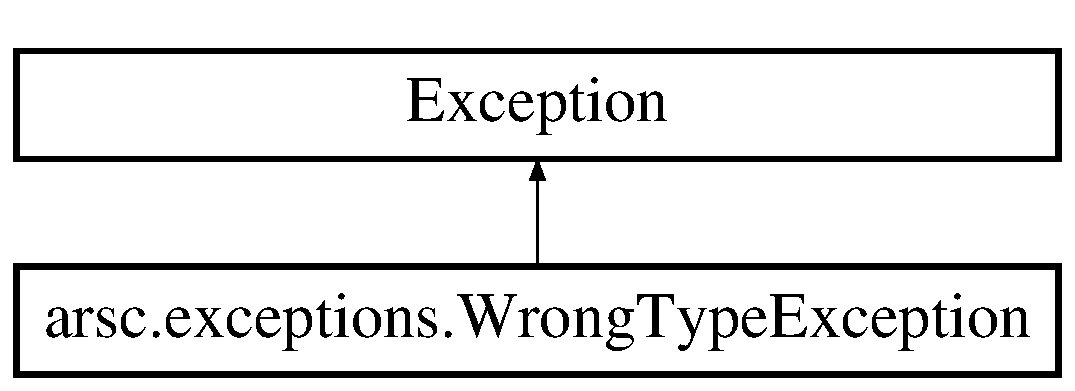
\includegraphics[height=2.000000cm]{classarsc_1_1exceptions_1_1WrongTypeException}
\end{center}
\end{figure}
\subsection*{Public Member Functions}
\begin{DoxyCompactItemize}
\item 
\mbox{\Hypertarget{classarsc_1_1exceptions_1_1WrongTypeException_a845a791c5e89bc7eadce30b501fbcf98}\label{classarsc_1_1exceptions_1_1WrongTypeException_a845a791c5e89bc7eadce30b501fbcf98}} 
def {\bfseries \+\_\+\+\_\+init\+\_\+\+\_\+} (self, field, header\+Type)
\end{DoxyCompactItemize}


The documentation for this class was generated from the following file\+:\begin{DoxyCompactItemize}
\item 
arsc/\mbox{\hyperlink{exceptions_8py}{exceptions.\+py}}\end{DoxyCompactItemize}

\chapter{File Documentation}
\hypertarget{arsc_8py}{}\section{arsc/arsc.py File Reference}
\label{arsc_8py}\index{arsc/arsc.\+py@{arsc/arsc.\+py}}


Main resource table functionality.  


\subsection*{Classes}
\begin{DoxyCompactItemize}
\item 
class \mbox{\hyperlink{classarsc_1_1arsc_1_1ResTable}{arsc.\+arsc.\+Res\+Table}}
\end{DoxyCompactItemize}


\subsection{Detailed Description}
Main resource table functionality. 


\hypertarget{chunk_8py}{}\section{arsc/chunk.py File Reference}
\label{chunk_8py}\index{arsc/chunk.\+py@{arsc/chunk.\+py}}


Res\+Chunk and related.  


\subsection*{Classes}
\begin{DoxyCompactItemize}
\item 
class \mbox{\hyperlink{classarsc_1_1chunk_1_1ResChunk__header}{arsc.\+chunk.\+Res\+Chunk\+\_\+header}}
\begin{DoxyCompactList}\small\item\em Header that appears at the front of every data chunk in a resource. \end{DoxyCompactList}\end{DoxyCompactItemize}


\subsection{Detailed Description}
Res\+Chunk and related. 


\hypertarget{config_8py}{}\section{arsc/config.py File Reference}
\label{config_8py}\index{arsc/config.\+py@{arsc/config.\+py}}


Res\+Table\+\_\+config and related.  


\subsection*{Classes}
\begin{DoxyCompactItemize}
\item 
class \mbox{\hyperlink{classarsc_1_1config_1_1ResTable__config}{arsc.\+config.\+Res\+Table\+\_\+config}}
\begin{DoxyCompactList}\small\item\em Describes current Res\+Table\+\_\+type configuration. \end{DoxyCompactList}\item 
class \mbox{\hyperlink{classarsc_1_1config_1_1ResTable__config_1_1Imsi}{arsc.\+config.\+Res\+Table\+\_\+config.\+Imsi}}
\begin{DoxyCompactList}\small\item\em Filter based on M\+CC and M\+NC. \end{DoxyCompactList}\item 
class \mbox{\hyperlink{classarsc_1_1config_1_1ResTable__config_1_1Locale}{arsc.\+config.\+Res\+Table\+\_\+config.\+Locale}}
\begin{DoxyCompactList}\small\item\em Filter based on language and country. \end{DoxyCompactList}\item 
class \mbox{\hyperlink{classarsc_1_1config_1_1ResTable__config_1_1ScreenType}{arsc.\+config.\+Res\+Table\+\_\+config.\+Screen\+Type}}
\item 
class \mbox{\hyperlink{classarsc_1_1config_1_1ResTable__config_1_1Input}{arsc.\+config.\+Res\+Table\+\_\+config.\+Input}}
\item 
class \mbox{\hyperlink{classarsc_1_1config_1_1ResTable__config_1_1ScreenSize}{arsc.\+config.\+Res\+Table\+\_\+config.\+Screen\+Size}}
\item 
class \mbox{\hyperlink{classarsc_1_1config_1_1ResTable__config_1_1Version}{arsc.\+config.\+Res\+Table\+\_\+config.\+Version}}
\item 
class \mbox{\hyperlink{classarsc_1_1config_1_1ResTable__config_1_1ScreenConfig}{arsc.\+config.\+Res\+Table\+\_\+config.\+Screen\+Config}}
\item 
class \mbox{\hyperlink{classarsc_1_1config_1_1ResTable__config_1_1ScreenSizeDp}{arsc.\+config.\+Res\+Table\+\_\+config.\+Screen\+Size\+Dp}}
\item 
class \mbox{\hyperlink{classarsc_1_1config_1_1ResTable__config_1_1Config}{arsc.\+config.\+Res\+Table\+\_\+config.\+Config}}
\end{DoxyCompactItemize}


\subsection{Detailed Description}
Res\+Table\+\_\+config and related. 


\hypertarget{exceptions_8py}{}\section{arsc/exceptions.py File Reference}
\label{exceptions_8py}\index{arsc/exceptions.\+py@{arsc/exceptions.\+py}}


libarsc exceptions  


\subsection*{Classes}
\begin{DoxyCompactItemize}
\item 
class \mbox{\hyperlink{classarsc_1_1exceptions_1_1WrongTypeException}{arsc.\+exceptions.\+Wrong\+Type\+Exception}}
\item 
class \mbox{\hyperlink{classarsc_1_1exceptions_1_1ChunkHeaderWrongTypeException}{arsc.\+exceptions.\+Chunk\+Header\+Wrong\+Type\+Exception}}
\end{DoxyCompactItemize}


\subsection{Detailed Description}
libarsc exceptions 


\hypertarget{configuration_8py}{}\section{arsc/external/configuration.py File Reference}
\label{configuration_8py}\index{arsc/external/configuration.\+py@{arsc/external/configuration.\+py}}


Android configuration bits.  


\subsection*{Classes}
\begin{DoxyCompactItemize}
\item 
class \mbox{\hyperlink{classarsc_1_1external_1_1configuration_1_1AConfiguration}{arsc.\+external.\+configuration.\+A\+Configuration}}
\end{DoxyCompactItemize}


\subsection{Detailed Description}
Android configuration bits. 


\hypertarget{package_8py}{}\section{arsc/package.py File Reference}
\label{package_8py}\index{arsc/package.\+py@{arsc/package.\+py}}


Res\+Table\+\_\+package and related.  


\subsection*{Classes}
\begin{DoxyCompactItemize}
\item 
class \mbox{\hyperlink{classarsc_1_1package_1_1ResTable__package__header}{arsc.\+package.\+Res\+Table\+\_\+package\+\_\+header}}
\begin{DoxyCompactList}\small\item\em A collection of resource data types within a package. \end{DoxyCompactList}\item 
class \mbox{\hyperlink{classarsc_1_1package_1_1ResTable__package}{arsc.\+package.\+Res\+Table\+\_\+package}}
\begin{DoxyCompactList}\small\item\em Describes whole package, together with its content. \end{DoxyCompactList}\end{DoxyCompactItemize}


\subsection{Detailed Description}
Res\+Table\+\_\+package and related. 


\hypertarget{stringpool_8py}{}\section{arsc/stringpool.py File Reference}
\label{stringpool_8py}\index{arsc/stringpool.\+py@{arsc/stringpool.\+py}}


Res\+String\+Pool and related.  


\subsection*{Classes}
\begin{DoxyCompactItemize}
\item 
class \mbox{\hyperlink{classarsc_1_1stringpool_1_1ResStringPool__header}{arsc.\+stringpool.\+Res\+String\+Pool\+\_\+header}}
\begin{DoxyCompactList}\small\item\em Definition for a pool of strings. \end{DoxyCompactList}\item 
class \mbox{\hyperlink{classarsc_1_1stringpool_1_1ResStringPool__header_1_1Flags}{arsc.\+stringpool.\+Res\+String\+Pool\+\_\+header.\+Flags}}
\item 
class \mbox{\hyperlink{classarsc_1_1stringpool_1_1ResStringPool}{arsc.\+stringpool.\+Res\+String\+Pool}}
\end{DoxyCompactItemize}


\subsection{Detailed Description}
Res\+String\+Pool and related. 


\hypertarget{table_8py}{}\section{arsc/table.py File Reference}
\label{table_8py}\index{arsc/table.\+py@{arsc/table.\+py}}


Res\+Table and related.  


\subsection*{Classes}
\begin{DoxyCompactItemize}
\item 
class \mbox{\hyperlink{classarsc_1_1table_1_1ResTable__header}{arsc.\+table.\+Res\+Table\+\_\+header}}
\begin{DoxyCompactList}\small\item\em Header for a resource table. \end{DoxyCompactList}\end{DoxyCompactItemize}


\subsection{Detailed Description}
Res\+Table and related. 


\hypertarget{align_8py}{}\section{arsc/type/align.py File Reference}
\label{align_8py}\index{arsc/type/align.\+py@{arsc/type/align.\+py}}


alignment function  


\subsection*{Functions}
\begin{DoxyCompactItemize}
\item 
def \mbox{\hyperlink{align_8py_a732cf485922fef2c1262bd8975f20f1f}{arsc.\+type.\+align.\+align}} (b, alignment=4)
\item 
def \mbox{\hyperlink{align_8py_a91355e3a94e9b8706d3dcb273e2568bd}{arsc.\+type.\+align.\+unalign}} (b, alignment=4)
\end{DoxyCompactItemize}


\subsection{Detailed Description}
alignment function 



\subsection{Function Documentation}
\mbox{\Hypertarget{align_8py_file_a732cf485922fef2c1262bd8975f20f1f}\label{align_8py_file_a732cf485922fef2c1262bd8975f20f1f}} 
\index{align.\+py@{align.\+py}!align@{align}}
\index{align@{align}!align.\+py@{align.\+py}}
\subsubsection{\texorpdfstring{align()}{align()}}
{\footnotesize\ttfamily def arsc.\+type.\+align.\+align (\begin{DoxyParamCaption}\item[{}]{b,  }\item[{}]{alignment = {\ttfamily 4} }\end{DoxyParamCaption})}

\begin{DoxyVerb}Returns bytes object aligned to specified number of bytes\end{DoxyVerb}
 \mbox{\Hypertarget{align_8py_file_a91355e3a94e9b8706d3dcb273e2568bd}\label{align_8py_file_a91355e3a94e9b8706d3dcb273e2568bd}} 
\index{align.\+py@{align.\+py}!unalign@{unalign}}
\index{unalign@{unalign}!align.\+py@{align.\+py}}
\subsubsection{\texorpdfstring{unalign()}{unalign()}}
{\footnotesize\ttfamily def arsc.\+type.\+align.\+unalign (\begin{DoxyParamCaption}\item[{}]{b,  }\item[{}]{alignment = {\ttfamily 4} }\end{DoxyParamCaption})}

\begin{DoxyVerb}Returns bytes after end of alignment to specified number of bytes\end{DoxyVerb}
 
\hypertarget{enum_8py}{}\section{arsc/type/enum.py File Reference}
\label{enum_8py}\index{arsc/type/enum.\+py@{arsc/type/enum.\+py}}


enumeration type  


\subsection*{Classes}
\begin{DoxyCompactItemize}
\item 
class \mbox{\hyperlink{classarsc_1_1type_1_1enum_1_1Enum}{arsc.\+type.\+enum.\+Enum}}
\end{DoxyCompactItemize}


\subsection{Detailed Description}
enumeration type 


\hypertarget{flag_8py}{}\section{arsc/type/flag.py File Reference}
\label{flag_8py}\index{arsc/type/flag.\+py@{arsc/type/flag.\+py}}


flag type  


\subsection*{Classes}
\begin{DoxyCompactItemize}
\item 
class \mbox{\hyperlink{classarsc_1_1type_1_1flag_1_1Flag}{arsc.\+type.\+flag.\+Flag}}
\end{DoxyCompactItemize}


\subsection{Detailed Description}
flag type 


\hypertarget{uint16_8py}{}\section{arsc/type/uint16.py File Reference}
\label{uint16_8py}\index{arsc/type/uint16.\+py@{arsc/type/uint16.\+py}}


Unsigned 16-\/bit Integer.  


\subsection*{Classes}
\begin{DoxyCompactItemize}
\item 
class \mbox{\hyperlink{classarsc_1_1type_1_1uint16_1_1uint16}{arsc.\+type.\+uint16.\+uint16}}
\end{DoxyCompactItemize}


\subsection{Detailed Description}
Unsigned 16-\/bit Integer. 


\hypertarget{uint24_8py}{}\section{arsc/type/uint24.py File Reference}
\label{uint24_8py}\index{arsc/type/uint24.\+py@{arsc/type/uint24.\+py}}


Unsigned 24-\/bit Integer.  


\subsection*{Classes}
\begin{DoxyCompactItemize}
\item 
class \mbox{\hyperlink{classarsc_1_1type_1_1uint24_1_1uint24}{arsc.\+type.\+uint24.\+uint24}}
\end{DoxyCompactItemize}


\subsection{Detailed Description}
Unsigned 24-\/bit Integer. 


\hypertarget{uint32_8py}{}\section{arsc/type/uint32.py File Reference}
\label{uint32_8py}\index{arsc/type/uint32.\+py@{arsc/type/uint32.\+py}}


Unsigned 32-\/bit Integer.  


\subsection*{Classes}
\begin{DoxyCompactItemize}
\item 
class \mbox{\hyperlink{classarsc_1_1type_1_1uint32_1_1uint32}{arsc.\+type.\+uint32.\+uint32}}
\end{DoxyCompactItemize}


\subsection{Detailed Description}
Unsigned 32-\/bit Integer. 


\hypertarget{uint64_8py}{}\section{arsc/type/uint64.py File Reference}
\label{uint64_8py}\index{arsc/type/uint64.\+py@{arsc/type/uint64.\+py}}


Unsigned 64-\/bit Integer.  


\subsection*{Classes}
\begin{DoxyCompactItemize}
\item 
class \mbox{\hyperlink{classarsc_1_1type_1_1uint64_1_1uint64}{arsc.\+type.\+uint64.\+uint64}}
\end{DoxyCompactItemize}


\subsection{Detailed Description}
Unsigned 64-\/bit Integer. 


\hypertarget{uint8_8py}{}\section{arsc/type/uint8.py File Reference}
\label{uint8_8py}\index{arsc/type/uint8.\+py@{arsc/type/uint8.\+py}}


Unsigned 8-\/bit Integer.  


\subsection*{Classes}
\begin{DoxyCompactItemize}
\item 
class \mbox{\hyperlink{classarsc_1_1type_1_1uint8_1_1uint8}{arsc.\+type.\+uint8.\+uint8}}
\end{DoxyCompactItemize}


\subsection{Detailed Description}
Unsigned 8-\/bit Integer. 


\hypertarget{types_8py}{}\section{arsc/types.py File Reference}
\label{types_8py}\index{arsc/types.\+py@{arsc/types.\+py}}


resource types in A\+R\+SC file  


\subsection*{Classes}
\begin{DoxyCompactItemize}
\item 
class \mbox{\hyperlink{classarsc_1_1types_1_1ResourceType}{arsc.\+types.\+Resource\+Type}}
\end{DoxyCompactItemize}


\subsection{Detailed Description}
resource types in A\+R\+SC file 


%--- End generated contents ---

% Index
\backmatter
\newpage
\phantomsection
\clearemptydoublepage
\addcontentsline{toc}{chapter}{Index}
\printindex

\end{document}
